\documentclass[12pt, b5paper,twoside]{tesi_upf}

%CODIFICATION
\usepackage[utf8]{inputenc}
\usepackage[T1]{fontenc}

%LENGUAGE
\usepackage[english,catalan]{babel}

%ONLY TO OBTAIN MARK BANK INDEX INDICATION B5
\usepackage[b5paper]{geometry}
% this needs to be removed eventually
%\usepackage[cam,a4,center,frame]{crop}

%INCLUDE GRAPHICS AND THE LOGO OF THE UPF
\usepackage{graphicx}

%% OTHER INCLUDES
\usepackage{booktabs}
\usepackage{rotating}
\usepackage[noend]{algpseudocode} % Algorithms
\usepackage{amsmath}
\usepackage{pdflscape}
\usepackage{appendix}
\usepackage{csvsimple}
\usepackage[usestackEOL]{stackengine}
\usepackage{subfig}
\usepackage{array}
\usepackage{float}
\usepackage{amssymb}
\usepackage{nameref}
\usepackage{xurl}
\usepackage[table]{xcolor}
\usepackage{caption}
\usepackage[table]{xcolor}
\usepackage{gensymb}
\usepackage{xparse}   % http://ctan.org/pkg/xparse
\usepackage{multirow}
\usepackage{diagbox} %table split headers

\newcolumntype{L}[1]{>{\raggedright\let\newline\\\arraybackslash\hspace{0pt}}m{#1}}
\newcolumntype{C}[1]{>{\centering\let\newline\\\arraybackslash\hspace{0pt}}m{#1}}
\newcolumntype{R}[1]{>{\raggedleft\let\newline\\\arraybackslash\hspace{0pt}}m{#1}}
\newcolumntype{P}[1]{>{\centering\arraybackslash}p{#1}}
\newcolumntype{M}[1]{>{\centering\arraybackslash}m{#1}}

\makeatletter
\def\@fnsymbol#1{\ensuremath{\ifcase#1\or \dagger\or
    \mathsection\or \mathparagraph\or \|\or **\or \dagger\dagger
    \or \ddagger\ddagger \else\@ctrerr\fi}}
\makeatother

\captionsetup[table]{skip=10pt}

%FONTS TIMES OR GARAMOND, 
\usepackage{times}
%\usepackage{garamond}

%WITHOUT HEADINGS: NO MODIFICATION
\usepackage{fancyhdr}

\fancyhead{}
\fancyfoot{}
\setlength{\headheight}{15pt}

%\renewcommand{\headrulewidth}{0.4pt}
\fancyhead[LO]{\footnotesize\slshape \rightmark}
\fancyhead[RE]{\footnotesize\slshape \leftmark}
\fancyhead[RO]{\iffloatpage{\thepage}{\thepage}}
\fancyhead[LE]{\iffloatpage{\thepage}{\thepage}}

%\fancyfoot[C]{\iffloatpage{}{\thepage}}
\pagestyle{fancy}

%FOR THE INDEX OF SUBJECTS
\usepackage{makeidx}
\makeindex

%%% CHAPTERPAGE
%\renewcommand{\chaptermark}[1]{\markboth{\MakeUppercase{#1}}{}}

%BIBLIOGRAPHY STYLE
%\bibliographystyle{numeric}
\bibliographystyle{vancouver}

%SELECT LANGUAGE
\selectlanguage{english}

%THE TABLE OF CONTENTS IS TITLE CONTENTS
\addto\captionscatalan
  {\renewcommand{\contentsname}{\Large \sffamily Sumari}}

%% MACRO TO CREATE FOOTNOTE WITHOUT NUMBERS
\makeatletter
\def\blfootnote{\xdef\@thefnmark{}\@footnotetext}
\makeatother

%ADD YOUR DATA
\title{Data-driven methods to characterize heterogeneity in Alzheimer’s disease using cross-sectional and longitudinal data}
\subtitle{}
\author{Gerard Martí Juan}
\thyear{2021}
\department{Department of Information and Communication Technologies}
\supervisor{Prof. Gemma Piella and Dr. Gerard Sanromà}

\begin{document}

\frontmatter
\maketitle

\cleardoublepage

%%%%%% Dedication

%\noindent 

%\cleardoublepage

%%%%%% End dedication

%%%%%% Thanks
\noindent {\Large \sffamily Agraïments} \\
Aquesta tesi és el resultat de quatre anys de feina, en els que he après moltíssimes coses i he crescut molt personalment i professionalment. No hagués pogut escriure aquesta tesi sense l'ajuda de moltíssimes persones. \\

En primer lloc, agrair enormement la feina dels meus supervisors, Gerard i Gemma, per les seves idees, suggeriments, i estar sempre disponible per qualsevol pregunta, correcció o el que necessités i per tenir sempre una actitud positiva, tan quan les coses sortien bé com quan no. Ha estat un gust enorme treballar plegats. \\

També vull donar les gràcies al Marco Lorenzi, d'INRIA, per donar-me la oportunitat d'anar un mes a fer una estada doctoral al seu grup. Enmig d'una pandèmia mundial, em va donar totes les facilitats del món per poder anar-hi i aprofitar-ho al màxim, i tot i que no vaig poder quedar-m'hi més temps, va ser una gran experiència. \\

Aquests 4 anys a la UPF (3 presencials, i 1 a distància, per desgràcia) no haguéssin estat el mateix sense la gent amb la que he compartit el dia a dia. Des dels que hi eren quan vaig arribar, fins als que han arribat després. El botó de bullshit, tardes interminables, cafès al Daniel, rates per la oficina, els dinars amb els microones que no calentaven, discussions sobre futbol (en les que sempre tenia raó), les calçotades, cerveses a l'Atrium. Gràcies a tots. Us he trobat a faltar aquest maleït any. Tornarem a trobar-nos, quan tot acabi. \\

No sembla que faci tant de temps que començavem l'escola, l'institut, o que compartíem els primers dinars al Penya. Després de tants anys, i amb tants d'altres per endavant, em sento molt afortunat de tenir amics que fan que tot això valgui la pena. Enrere queden hores impagables jugant a videojocs, fent cerveses, compartint moments, conversant, compartint memes absurds, rient. Encara ens queda molt per endavant. Keep moving forward. \\

Tinc la sort de tenir una gran família. Als meus avis, tiets i cosins, gràcies per ser-hi sempre. I als meus pares i a la meva germana, per donar-me sempre suport en tot el que he decidit fer a la vida (i per suportar-me aquests últims mesos de pandèmia). Gràcies Papa, Mama, i Aina. Us estimo molt. \\

Per acabar, el dia més important d'aquests últims 4 anys no serà el dia de la defensa de tesi, sinó el 8 de Març de 2017, i no precisament per fotre-li 6 gols al PSG. Gràcies per ser com ets i fer-me tan feliç. Sense tu, estaria perdut. T'estimo molt, Núria. \\

\cleardoublepage

%%%%%% End of thanks

%ABSTRACT IN TWO LEGUAGES.
\selectlanguage{english}
\section*{\Large \sffamily Abstract}
% INITIAL REQUERIMENT IS TO USE LESS THAN 150 WORDS.
Alzheimer's disease (AD), the most common form of dementia, is an incurable neurodegenerative disease that affects millions of elderly people worldwide. Detecting the disease in its early stages is the key for a more effective treatment. AD is a multifactorial disease, where several markers represent different pathophysiological processes in the brain, with distinct progression paths over time. Methods to facilitate the integration and interpretation of longitudinal, heterogeneous medical data could be of benefit for a better understanding of the disease and its progression. In this thesis, we present statistical and machine learning methods and studies for early detection and to assess disease progression. \\

Contributions of this thesis are as follows: First, we present a review on machine learning applications in AD using longitudinal neuroimaging: we analyze their approach to typical challenges in longitudinal data analysis and show that machine learning methods using longitudinal data have potential to improve disease progression modelling and computer-aided diagnosis. Our second contribution is a study of AD subtyping using novel plasma-based blood markers. We used a multivariate, multiple kernel learning embedding method over blood-based markers to find subgroups of patients defined by distinctive blood marker profiles, and we analyze those subgroups using cross-sectional and longitudinal neuroimaging data. Our third contribution is a novel method based on recurrent, multimodal variational autoencoders to model the progression of the disease. It can use a variable number of modalities and time-points across different subjects, and we show its performance quantitatively and qualitatively. Our fourth and final contribution is an analysis of the impact of APOE $\varepsilon4$ gene dose and its association with age on hippocampal shape, assessed with multivariate surface analysis, using a $\varepsilon4$-enriched cohort.

\selectlanguage{catalan}
\vspace*{\fill}
\section*{\Large \sffamily  Resum}
La malaltia d'Alzheimer, o simplement alzhèimer, és una malaltia neurodegenerativa incurable que afecta milions de persones a tot el món. La detecció de la malaltia en els seus primers estadis és clau per a un tractament més eficaç. L’alzhèimer és una malaltia multifactorial, on diversos marcadors representen processos fisiopatològics diferents al cervell, amb diferents tipus de progressió al llarg del temps. Mètodes per facilitar la integració i la interpretació de dades mèdiques longitudinals i heterogènies poden ser útils per aconseguir una millor comprensió de la malaltia i la seva progressió. En aquesta tesi presentem mètodes estadístics i d’aprenentatge automàtic per a la detecció precoç i per avaluar la progressió de la malaltia. \\

Les contribucions d’aquesta tesi són les següents: En primer lloc, presentem una revisió de mètodes d’aprenentatge automàtic aplicats a l'alzhèimer que utilitza dades de neuroimatge longitudinals: analitzem el seu enfocament als desafiaments típics en l’anàlisi d'aquestes dades i demostrem que els mètodes d’aprenentatge automàtic que utilitzen dades longitudinals tenen potencial per a millorar la modelització de la progressió de la malaltia i el diagnòstic assistit per ordinador. La nostra segona contribució és un estudi de subtipatge de l'alzhèimer mitjançant marcadors sanguinis basats en plasma. Utilitzem un mètode multivariat i no supervisat en marcadors sanguinis per trobar subgrups de pacients definits per perfils distintius d'aquests marcadors, i analitzem aquests subgrups utilitzant dades de neuroimatge transversal i longitudinal. La nostra tercera contribució és un mètode basat en "recurrent variational autoencoders", un tipus de xarxa neuronal, per modelar la progressió de la malaltia. El mètode utilitza un nombre variable de modalitats i punts de temps en diferents pacients, i mostrem el seu rendiment quantitativament i qualitativament. La nostra quarta i última contribució és una anàlisi de l’impacte de la dosi del gen APOE $\varepsilon4$ i la seva associació amb l’edat en la forma de l’hipocamp, evaluada amb un anàlisi de superfície multivariada sobre una cohort amb alta proporció de pacients amb el gen $\varepsilon4$.
\vspace*{\fill}

\cleardoublepage
%END OF ABSTRACT
\selectlanguage{english}

%PREFACE. 
% PREFACE AND THANKS ARE THE SAME, RIGHT
%{\bf Preface} % que es aixo lmao

%\cleardoublepage
%END OF PREFACE

%TABLE OF CONTENTS: REQUIRED
\tableofcontents

%lIST OF FIGURES; ONLY IF THERE ARE FIGURES
\listoffigures
%TO APPER THE LIST OF FIGURES IN THE TABLE OF CONTENTS 
\addcontentsline{toc}{chapter}{List of figures}

%LIST OF TABLES; ONLY IF THERE ARE TABLES
\listoftables
%TO APPEAR THE LIST OF TABLES IN THE TABLE OF CONTENTS
\addcontentsline{toc}{chapter}{List of tables}

%START THE TEXT
\mainmatter

\chapter{Introduction} \label{ch:1-introduction}

%%% INITIAL SUMMARY

The study of neurodegenerative diseases such as Alzheimer's disease (AD) usually entails gathering different markers of the disease coming from different sources or metodologies \cite{Jack2010}: brain imaging techniques, cognitive assessments, or cerebrospinal fluid punctures. Over the past decades, such techniques have become widespread and there has been a surge on the number of available data. Large datasets from patients at different stages of the disease containing heterogeneous and over time (longitudinal) data could help unravel unseen mechanisms and provide insights on its evolution. However, we need novel methods that can leverage and extract meaningful information from such complex data. \\

Machine learning (ML) is a set of techniques and models that have shown strong performance on a variety of tasks. These techniques are closely related to statistical methods and have gained a lot of popularity recently with the advent of deep learning (DL) \cite{LeCun2015}. ML and DL techniques have been applied to medical data, including AD \cite{Litjens2017,Ching2018}. The field still faces many challenges, and it will keep developing over the next years. An important challenge is to build methods that are able to find relationships between different markers to improve our understanding of the progression of the disease. In this thesis, we explore machine learning and statistical methods that are able to help us gain insight on different aspects of AD using heterogeneous, longitudinal medical data. \\

\section{Alzheimer's disease}

% Severity of Alzheimer's Disease.
AD is an incurable neurodegenerative disease that causes a progressive degeneration of the brain and cognitive functions \cite{Lane2018}. Our current understanding is that the disease is characterized by an accumulation of amyloid-beta (A$\beta$) proteins in the brain and the formation of tau plaques, that causes brain atrophy and gradually impair the cognition of the patients, and finally leading to death \cite{Ballard2011}. AD affects more than 47 million people worldwide, generating an estimated healthcare cost of around 604 billion US dollars a year \cite{AlzheimersAssociation}. As AD is a disease that generally affects elderly people, and accounting for the general aging of the population, this impact will only get stronger. It is estimated that, by 2030, 76 million people worldwide could be affected by this disease \cite{AlzheimersAssociation}. \\

%% Small paragraph on the difference between familial AD and late onset AD.
Generally, when we talk about AD we refer to sporadic late-onset AD, which has no known cause. There also exists a variant named autosomal dominant familial AD, affecting less than $5\%$ of AD patients \cite{Bird1993}, which is caused by genetic mutations on APP, PSEN1 and PSEN2 genes \cite{Campion1999}. It has an earlier age of onset, but it has a similar clinical presentation compared to its sporadic, most common form \cite{Ryan2016}. All the work contained in this thesis is only applied to late-onset AD, and from now on it will be referenced in the text as AD for simplicity. \\

%% use marinescus thesis citations
Up to now, there has been no successful treatment to cure or slow down the cognitive decline caused by AD. Despite all the research on the topic, all clinical trials have failed \cite{Mehta2017} and did not manage to prove efficacy, even recent ones \cite{Huang2020}. Failures in drug design and development for AD could be linked to many reasons. One is that our understanding of the underlying processes that initially cause the cascade of events leading to the disease still needs to improve. Another reason could be that any potential successful drug would need to be administered at a presymptomatic stage of AD \cite{Mehta2017,Huang2020}. Detection of cognitively healthy patients at risk, or patients with very mild impairment that will progress to AD in the future is of utmost importance for future drugs and trials. \\ 

In the literature, diagnosis of patients is usually divided in three stages \cite{Brookmeyer2007}, although other classifications have been recently proposed \cite{Jack2018}:

\begin{enumerate}\itemsep5pt
\item Healthy control or cognitively normal (CN), when the patient shows neither signs of the disease nor cognitive problems.
\item Mild cognitive impairment (MCI), when the patient shows signs of cognitive impairment. It can be divided into two substages: early MCI and late MCI, differentiating between patients by their degree of cognitive impairment.
\item AD, when the patient is considered to have completely progressed into full-blown dementia.
\end{enumerate}

\subsection{AD markers}

To determine the current stage of the disease, various markers describing key pathophysiological processess of AD have been proposed over the years. AD is a multifactorial disease, with distinct progression paths depending on the used markers. AD is characterized by protein amyloid-beta (A$\beta$) deposition in the brain \cite{Rissman2012}, tau injury, and structural neurodegeneration \cite{Jack2013}. Those three indicators precede cognitive impairment, leading to death. For the measurement of these indicators, different markers have been proposed:

\begin{enumerate}\itemsep5pt
\item Brain A$\beta$ deposition in the brain can be detected both in positron emission tomography (PET) imaging \cite{Clark2011}, and in cerebrospinal fluid (CSF) \cite{Andreasen1999}.
\item Tau injury and dysfunction caused by tau and p-tau plaques, found in tau-PET imaging and CSF \cite{Andreasen1999,Blennow2010}.
\item Neurodegeneration provoked by tau injury. It can be observed in structural magnetic resonance imaging (MRI) \cite{Weiner2005} and in fludeoxyglucose (FDG)-PET imaging \cite{Chetelat2003}.
\item Memory and cognition, measured by cognitive tests.
\end{enumerate}

%% Screening
The main screening tool for clinical assessment of AD is the clinical interview between the patient and the doctor, where the severity of the cognitive problems of the patient can be assessed, followed by a cognitive physical examination to capture the aforementioned markers and assess the presence of the disease \cite{Lane2018}. \\

%% Blood based
Apart from the aforementioned markers and imaging techniques, blood based markers have also been proposed for AD diagnosis \cite{Shi2018}, as they potentially could be a non-invasive, cheaper way to diagnose. Recently, plasma marker p-tau181 has shown promising results for an accurate AD diagnosis \cite{Karikari2020}. \\

%% APOE
AD has also been linked to several genetic mutation risks. Apart from the genes linked to previously mentioned autosomal familial AD, the major genetic risk factor for AD is the Apolipoprotein E (APOE) $\varepsilon$4 allele \cite{Saunders1993}. It has been linked to an increased risk of AD, depending on allele load (if the patient has one or two copies of the allele) \cite{Liu2013a}.

\subsection{Longitudinal marker dynamics and disease model}

The previous markers can be studied and modelled longitudinally. Modelling their trajectories and progression can give us more insight on how they change and interact. For example, longitudinal data analysis on MRI allows us to calculate the rate of change of specific brain structures, such as the dynamics of cortical and hippocampal atrophy. \\

A widely accepted progression model of AD was proposed by \cite{Jack2010}. Their model is based on marker evolution, where each marker progresses from normal values to abnormal values differently. The order of the markers is the presented above: A$\beta$ deposition, followed by tau injury, neurodegeneration and cognition. Empirical data and experiments reviewed in \cite{Jack2013} confirm the validity of the model, although other data-driven works do not fully agree with it \cite{Iturria-Medina2016}. \\

%% Explicar aqui una mica de AD subtyping, del paper de young, tal tal
AD is a highly heterogeneous disease. It can overlap with other neurological pathologies and presenting different paths of neurodegeneration, with different rates of atrophy for different areas of the brain \cite{Lam2013,Poulakis2018}, distinct clinical and cognitive characteristics \cite{Murray2011} or even differences in other more specific markers like CSF proteomics \cite{Tijms2020}. Development of methods to study the progression of AD should also take into account this heterogeneity for a better understanding of the disease. \\

\section{Challenges in longitudinal and heterogeneous data}

Longitudinal data are composed of sequential data acquisitions for subjects over a period of time. This contrasts with cross-sectional studies, which focus on single acquisitions per subject. Here, we describe the main characteristics and analysis challenges that arise while dealing with longitudinal data. \\

Two sources of variability can be defined for a longitudinal study in a cohort of subjects: the inter-subject variability, i.e., the differences between observations of different subjects, and the intra-subject variability, i.e., the differences between observations of a same subject, which tend to be highly correlated compared to the former. Those two sources of variation give valuable information about the progression of the disease between- and within- subjects. In cross-sectional studies, those two variabilities are non-separable: given two samples of different subjects, it is not possible to know to what extent their variation is due to inter-subject variability or to the different stages of the disease. Adding longitudinal samples for each subject allows us to distinguish between those two variabilities, improving our understanding of the disease \cite{Fitzmaurice2008}. \\

\begin{figure}[htbp]
  \centering
  \includegraphics[width=1.0\textwidth]{figures/introduction/Fig-progression.pdf}
  \caption{Longitudinal representation of data acquisitions for two patients.}
  \label{long}
\end{figure}

Figure \ref{long} shows an example of a longitudinal study for two subjects, with multiple data modalities, over a fixed span of time. It illustrates some of the challenges that can appear in a longitudinal, multimodal data study: \\

% The figure should include these various points
% \itemsep5pt was put originally but tal
\begin{enumerate}
\item Each subject can have a different number of acquisitions, leading to an unbalanced data problem. In the figure, Patient B missed the 12th month acquisition for some reasons.
\item There can be missing data due to missing acquisitions from some modalities. In the figure, only patient A at the 6-months follow-up has all the acquisitions.
\item Data are not necessarily acquired at the same time point for the different subjects.
\item Time spacing between follow-ups can be variable, even within a single subject.
\end{enumerate}

Another problem, not shown in the figure, is that different patients can be at different stages of the disease at a given time point. Reference time to measure progression remains an open issue in the field \cite{Ashford2001}.  \\

Protocols of data acquisition try to palliate these problems, but in a clinical setting, this is very difficult to achieve: sometimes patients miss their scheduled screening session and data cannot be gathered. Other patients might drop out from the study for a variety of reasons, such as disease severity or moving out of the city/country, and in other cases, data of a given time point could need to be discarded because of quality problems. For these reasons, most of the available longitudinal data is unbalanced. \\

\subsection{Studies and initiatives} 
%% Explain about studies that focus on longitudinal data. and about the challenges that promote the use of longitudinal data for progression of the disease.

There has been a remarkable number of initiatives to promote using longitudinal data on AD modelling. Availability of patients' longitudinal data is key to study the progression of the disease. Lawrence et al. \cite{Lawrence2017} presented a review of available longitudinal AD biomarker datasets, finding that more efforts are needed to increase the follow-up duration, increase the population sizes and standardize the acquisition methods. One of the largest studies is the Alzheimer's Disease Neuroimaging Initiative (ADNI) \cite{Mueller2005}, a multimodal, ongoing longitudinal study with hundreds of enrolled subjects, gathering imaging data, cognitive scores, blood and CSF markers. To unify and share the available data, the Alzheimer's Association has created The Global Alzheimer’s Association Interactive Network (GAAIN)\footnote{\url{http://www.gaain.org}} to share data between independent studies and build collaborations to create and explore large, heterogeneous cohorts. More recently, a new initiative named Alzheimer's Disease Data Initiative (ADD)\footnote{\url{https://www.alzheimersdata.org/}} have been created for similar reasons of data unification and sharing. \\

\section{Machine learning for medical data}

%% Introductory paragraph: general citations on healthcare: medical records, image segmentation, top results from google, etc.
Traditional methods for data analysis usually rely on searching relationships between measured quantities (e.g. variables). For example, in statistical inference, we start from a hypothesis of the effect of an independent variable on the dependent (output) variables, and look for relevant associations that confirm or refute the hypothesis. From another perspective, ML allows us to accurately model the relationship between input and output that generalize to unseen data. ML is particularly helpful when dealing with complex and unwieldy data, and when the number of input variables is large. Usually, ML models are trained for a specific task (e.g. image recognition, or diagnosis prediction), but such techniques are also very useful to find patterns or relationships in high-dimensional data that could not be found otherwise due to the inherently complex nature of it. Lately, DL has become one of the most used ML tools for high-dimensional data. \\

ML has been applied to many healthcare problems. For example, breast cancer screening \cite{McKinney2020} or predicting cardiovascular risk factor on retina images \cite{Poplin2018}, have shown strong results using ML based techniques. A very prolific application of ML is medical imaging, where it has been used for image classification, segmentation, or synthetic data generation \cite{Litjens2017}. Use of such techniques also raise important technical and ethical questions, such as privacy concerns over data usage \cite{Yang2019} or bias or transparency issues \cite{Karikari2020, Haibe-Kains2020}. Nonetheless, the results achieved show their strength and potential for problems with high-dimensional, complex medical data. \\

ML has also been used in AD research for several tasks, such as diagnosis classification \cite{Rathore2017}, disease progression modeling \cite{Oxtoby2017} or disease subtpying \cite{Young2017}, to name a few. The inherent complexity between the different modalities of markers of the disease and their temporal evolution and trajectories, coupled with the still unknown mechanisms underlying AD, make ML a prime candidate for the study of the disease. \\

%% Here, talk on the limitations of the current methods

\section{Contributions and outline of the thesis}

The main contributions of the thesis are presented in four main chapters, in addition to the introduction (Chapter \ref{ch:1-introduction}) and a final chapter with the general conclusions of our work (Chapter \ref{ch:6-conclusions}):

\begin{itemize}
    \item Chapter \ref{ch:2-review} reviews statistical and machine learning applications in AD using longitudinal neuroimaging. We perform a literature review of the field, selecting 105 papers to review. Our objective was to paint a clear picture of the state of the field, compare the current approaches and methods, and discover existing limitations. We show that methods that use longitudinal data have a strong potential for modelling disease progression and computer-aided diagnosis. 
    \item Chapter \ref{ch:3-cimlr} shows a study on AD subtyping using blood markers. We apply a non-supervised clustering approach, based on multiple kernel learning, to study AD subtyping using novel plasma markers. We obtain different subtypes of patients with different presentation of the disease, and we discover potential interactions between the groups using MRI based markers.
    \item Chapter \ref{ch:4-rnnvae} presents a generative model based on variational autoencoders and recurrent neural networks that is able to combine multimodal, longitudinal data, with variable number of time-points.This method can predict the evolution of a given patient, show relationships between modalities, and input missing channels. This is achieved by explicitly modelling the interdependencies between modalities, and using recurrent neural networks to model the evolution of each modality over time. We show the potential of the technique using synthetic and real data examples.
    \item Chapter \ref{ch:5-pmhippocampus} contains a study on the impact of APOE $\varepsilon$4 gene dose and its interaction with age on hippocampal shape, assessed with multivariate surface analysis, using an $\varepsilon$4-enriched cohort of cognitively unimpaired subjects. We discovered relevant non-linear interactions that show how the hippocampus is affected in APOE4 subjects, and found similarities with the effect of AD on hippocampal shape using a second cohort containing patients at all stages of the disease.
\end{itemize}

These four chapters of the thesis are self-contained and adapted from peer-reviewed journal articles, or from articles in preparation (Chapter \ref{ch:4-rnnvae}). The citation to the original article can be found on the first page of each chapter.

% \subsection{Biological definition of AD}
% A new unified research framework for a biological definition of the disease was recently published by the National Institute on Aging and the Alzheimer's Association \cite{Jack2018}. This approach defines AD as a biological construct based on markers, rather than clinical symptoms of the disease such as cognitive impairments. The framework is flexible enough for the introduction of additional markers, if needed. \\

% The framework groups markers in three categories: A$\beta$ deposition, pathologic tau, and neurodegeneration. This is represented as the AT(N) system, where each category can be binarized using a cut point into normal/abnormal (-/+). For each category:

% \begin{itemize}
%     \item \textbf{A:} A$\beta$ markers determine if a patient is in the Alzheimer's continuum, showing pathological changes but still not presenting the disease.
%     \item \textbf{T:} tau deposition markers indicate whether a patient who is in the Alzheimer's continuum has the disease.
%     \item \textbf{(N):} Neurodegeneration markers show structural changes in the brain that can be product of AD, but are not specific to the disease (and thus is placed in parenthese).
% \end{itemize}

% % Review of existing works and if there is anything longitudinal
% The flexibility of the framework allows working with missing biomarker values, which is a valuable trait for a longitudinal study. We found no work (within the scope of this review) using this new biological definition on AD. The reasons could be the recentness of the framework's publication, and the need for multimodal data in a longitudinal setting, which is not as available as single modality MRI. However, we expect future studies to use this framework, as it offers clear advantages for longitudinal analysis: for example, being able to directly compare different stages of progression between patients, or extend the framework with markers that capture longitudinal progression.


%%% AIXO HO HE TRET PERQUÈ ÉS INFORMACIÓ BASTANT SUPÈRFLUA I NO FA FALTA

% ADD MIRIAD Challenge
%Initiatives to stimulate research on the field have also been proposed, such as the MIRIAD challenge \cite{miriad}, The Alzheimer's Disease Prediction Of Longitudinal Evolution (TADPOLE) Challenge\footnote{\url{https://tadpole.grand-challenge.org}} or Quantitative Templates for the Progression of Alzheimer’s disease (QT-PAD)\footnote{\url{http://www.pi4cs.org/qt-pad-challenge}}. These challenges define a fixed subset of available data, making it easier to compare results, share methods and ensure reproducibility. \\


\chapter[A survey on machine and statistical learning for longitudinal analysis of neuroimaging data in Alzheimer’s Disease]{A survey on machine and statistical learning for longitudinal analysis of neuroimaging data in Alzheimer’s Disease} \label{ch:2-review}
\chaptermark{Survey on ML methods in longitudinal AD}
\blfootnote{Adapted from: Martí-Juan, G., Sanroma-Guell, G., Piella, G. (2020, June 1). A survey on machine and statistical learning for longitudinal analysis of neuroimaging data in Alzheimer’s disease. Computer Methods and Programs in Biomedicine, Vol. 189, p. 105348. \url{https://doi.org/10.1016/j.cmpb.2020.105348}}
\section{Introduction}

Alzheimer's disease (AD), the most common form of dementia, is an incurable neurodegenerative disease that affects millions of elderly people worldwide \cite{Ferri2005,Prince2013}. Cognitively normal (CN) subjects affected with the disease start to show progressive loss of memory and cognition \cite{Backman2004}, entering a mild cognitive impairment (MCI) stage, before developing to full-blown AD. Detecting the disease in its early stages is the key for a more effective treatment aimed at preventing the degenerative process.  \\

A better understanding of the disease progression is crucial for early diagnosis and personalized therapy. AD is described as a multifactorial disease \cite{Jack2010}, where several markers represent different pathophysiological processes in the brain, with distinct progression paths. Examples of such markers are brain A$\beta$ deposition, tau injury and neurodegeneration, and they can be used to analyze disease progression from different perspectives. \\ 

Due to the widespread use and availability of medical devices during the past decades, we now have access to electronic medical records containing a varied set of clinical data coming from multiple sources, including brain imaging scans from different modalities, acquired over time in a longitudinal fashion \cite{Lawrence2017}.  Contrary to cross-sectional studies, longitudinal studies allow us to measure the evolution and effects of phenotypic characteristics over time caused by disease progression \cite{Mills2014}. \\

Traditional methods of statistical data analysis for extracting knowledge rely on searching relationships among measured quantities (variables). Machine learning (ML) allows us to accurately model the relationship between input and output that generalize to unseen data. ML can particularly helpful when dealing with complex and unwieldy data, and when the number of input variables is large. One application of ML is prediction (e.g., diagnosis), but such techniques are also useful to find patterns or relationships in the data. Methodologically, the boundary between ML and statistical methods is fuzzy. We refer the reader to \cite{Breiman2001,Shmueli2010} for a more in-depth discussion. \\

%Traditional methods of data analysis for extracting knowledge rely on searching relationships among measured quantities (variables). In statistical inference, we start from a hypothesis of the effect of potential independent (input) variables on the dependent (output or outcome) variables, and look for above-chance associations that confirm or refute the hypothesized relation. Statistical modeling caters for prediction, but predictive accuracy is not its primary goal. From another perspective, machine learning (ML) allows us to accurately model the relationship between input and output that generalize to unseen data. ML is particularly helpful when dealing with complex and unwieldy data, and when the number of input variables is large. One application of ML is prediction (e.g., diagnosis), but such techniques are also useful to find patterns or relationships in the data. Methodologically, the boundary between ML and statistical methods is fuzzy. We refer the reader to \cite{Breiman2001,Shmueli2010} for a more in-depth discussion. \\

Progression of the disease using cross-sectional information has been examined by many ML studies \cite{Oxtoby2017,Acharya2019}. Fewer have used a sequence of acquisitions and assessed longitudinal changes directly. Although working with longitudinal data can improve our knowledge of the disease \cite{Xu2014}, adding a temporal dimension entails difficulties and data analysis problems, such as data imbalance or time alignment, that need to be addressed \cite{Fitzmaurice2008,Ibrahim}. \\

In this survey, we review current machine and statistical learning studies and identify trends for longitudinal medical imaging analysis, current gaps in the literature, and possible future directions. We divide the reviewed studies in two large groups: computer-aided diagnosis (CAD) and progression modelling. We exclude purely statistical inference studies, as our focus is on general-purpose learning techniques. We believe that such techniques can leverage longitudinal information and give new insights into AD and dementia progression, due to their ability to manage and explore growing volumes of diverse available data in an exploratory hypothesis-free setting.\\

%\begin{figure}[ht!]
%  \centering
%  \includegraphics[width=0.95\textwidth]{figures/review/paperoutline.png}
%  \caption{Outline of the review.}
%  \label{fig:overview}
%\end{figure}

% Rewrite this when the figure and the new sections are done
% Figure \ref{fig:overview} shows the outline of the paper. 
This paper is organized as follows: in Section \ref{sec:search}, we describe the search criteria used to gather the reviewed works. In Section \ref{sec:longdata} we discuss their data usage, focusing on the type of longitudinal data and measured markers. Next, we talk about the tasks addressed by the reviewed works: in Section \ref{sec:progression} we analyze works that model the progression of the disease, categorized by the main method used, and detail the advantages and disadvantages of the reviewed approaches. Then, in Section \ref{sec:classification}, we analyze papers focused on computer-aided diagnosis of the disease, describing both the methods and the data used, as well as their performance. We then discuss specific aspects: in Section \ref{sec:missing}, we explain how researchers handle certain problems such as temporal alignment and missing data approaches. In Section \ref{sec:bias} we discuss about the reproducibility and interpretability of the reviewed works. Finally, based on our analysis, in Section \ref{sec:conclusion} we discuss the overall results, draw conclusions, and suggest possible further research paths. \\

\section{Search methods}
\label{sec:search}

We reviewed works that 1) focus on AD or dementia, 2) use medical imaging derived markers, 3) use longitudinal data, and 4) use ML methods. We created four groups of keywords for the search:

\begin{itemize}\itemsep5pt
  \item \textbf{Keywords related to the disease:} Dementia, Alzheimer’s disease, Mild Cognitive Impairment, AD
  \item \textbf{Keywords related to markers of the disease:} MRI, PET, medical imaging, Magnetic resonance imaging, Positron emission tomography, fMRI, T1 MRI, T2 MRI, FLAIR, DWI
  \item \textbf{Keywords related to longitudinal data analysis:} longitudinal, spatiotemporal, temporal, long-term, follow-up, progression
  \item \textbf{Keywords related to machine learning and statistical learning methods:} classification, learning, prediction, data-driven, precision medicine, pattern recognition, artificial intelligence, AI, ML
\end{itemize}

The keywords were chosen to be general terms for each concept but specific enough to discard unrelated papers. We used the search engines of PubMed, ScienceDirect, Scopus, arXiv, and bioRxiv. In each website, we retrieved papers that had at least one keyword from each group. Depending on the website, its search engine did not allow to use the full search: that was the case in ScienceDirect, Scopus, and Biorxiv, where we had to reduce the number of terms. In these cases, we only used the first two words of each category, which we consider to be the most representative. \\

We excluded papers that were not related to AD or that did not use longitudinal imaging data in their experiments or models. We also excluded papers that did not use a general-purpose learning approach, as mentioned in the introduction. For example, statistical reports whose goal was to test a specific hypothesis. \\

Search was done over a period going from January 1st, 2007 to July 31st, 2019. We obtained a total of 1404 different papers. Then, we removed papers that were out of scope (1300). These include papers that did not use learning methods, that used only cross-sectional data, or that focused on other diseases, but had appeared in our search. After that, we removed duplicates from the remaining papers (44), leaving us with a total of 60 papers. Finally, we did a search on the references and citations of the selected papers to include relevant works that could have been missed by our initial search, adding up to \textbf{105} selected works. Figure \ref{fig:search} shows a diagram of the selection process.

\begin{figure}[!htbp]
  \centering
  \includegraphics[width=0.9\textwidth,height=0.9\textheight,keepaspectratio]{figures/review/Fig1.pdf}
  \caption{Paper selection pipeline.}
  \label{fig:search}
\end{figure}

\section{Data and methods usage}
\label{sec:longdata}

We analyzed the data and methods in the final selection of papers to gain an initial understanding of the reviewed works. We focused on several key aspects: follow-up length, measured markers, database, and main methods used. \\

\subsection{Follow-up length} 
 
 \begin{figure}[!htbp]
\centering
\includegraphics[width=0.75\textwidth]{figures/review/Fig2.pdf}
    \caption{Reviewed papers according to their reporting of follow-up length.}\label{fig:followupsdist}
\end{figure}
 
To assess the impact of longitudinal data used in a paper, we analyzed the number of follow-ups per subject and the follow-up length. Figure \ref{fig:followupsdist} shows how this information was reported in the reviewed articles. Most of them report enough information on the longitudinal data selection, with the majority of articles reporting both the maximum number of follow-ups and the average number of follow-ups, but a sizeable amount of articles did not report information about the years of follow-up. This can raise some concerns about reproducibility (see Section \ref{sec:bias}, and it affects the comparison with other works and the correct assessment of the methodology used. \\

Figure \ref{fig:followups} shows the distribution of the (maximum and/or average) number of follow-ups reported in the selected papers. We observe that the distribution is skewed at a low number of follow-ups, in both maximum- and average-number graphs. This is an expected result due to the limited availability of adequate long-term data: subjects having a large number of follow-ups are sparse in available longitudinal datasets \cite{Lawrence2017}. A substantial percentage of works ($39\%$, not counting those that did not report the information) use only one or two follow-ups in addition to the baseline. \\

\begin{figure}[!htbp]
\centering
\includegraphics[width=1.0\textwidth]{figures/review/Fig3.pdf}
    \caption[Distribution of the number of follow-ups used in the reviewed papers.]{Distribution of the number of follow-ups (maximum and average) used in the reviewed papers. Rounded average values. N: not reported.}\label{fig:followups}
\end{figure}

Figure \ref{fig:followups_years} shows the distribution of the (maximum and/or average) number of years of follow-up reported. In average, studies follow the patients for between 1 to 3 years, and for a maximum of 2 to 4 years. There is a small subset of papers that are very long term following the patient from 8 to 12 years \cite{Ghazi2019,Chen2012,Li2017b,Li2017c,Bilgel2015a,Bilgel2016}. Depending on the follow-up length, we distinguish between two groups:

\begin{figure}[!htbp]
\centering
\includegraphics[width=1.0\textwidth]{figures/review/Fig4.pdf}
    \caption[Distribution of the years of follow-up used in the reviewed papers.]{Distribution of the years of follow-up (maximum and average) used in the reviewed papers.}\label{fig:followups_years}
\end{figure}

\begin{itemize}\itemsep7pt

\item Short-term longitudinal works, including follow-ups up to, at maximum, two years. These papers tend to select a subset of available data, avoiding missing data and unbalanced data problems \cite{Ardekani2016,Fiot2012,Fiot2014,Gray2012,Rodrigues2014,Shi2015,Shi2017}. Papers based on short-term brain atrophy \cite{Huang2012,Hyun2016,McEvoy2011,Sanroma2017,Vounou2012}, where usually only one follow-up is needed to calculate tissue loss, and those using several modalities that want to avoid missing data problems \cite{Chen2011b,Hinrichs2011,Jack2009} tend to be short-term.

\item Long-term longitudinal works, including follow-ups of three years or more. These papers need to deal with missing data, as long-term data tend to be sparse. However, long-term data give an additional insight into the whole progression of the disease that short-term longitudinal data cannot provide. There are many disease progression studies using long-term longitudinal data \cite{Desikan2011,Guillaume2014,Guerrero2016,Bilgel2015a,Bilgel2016,Iturria-Medina2016,Li2017b,Aghili2018}, whereas computer-aided diagnosis works using long-term longitudinal data are less common \cite{Chi2017,Minhas2016}. Some works use longer-term longitudinal data for model validation after training on a short-term subset \cite{Young2015a}.
\end{itemize}

As mentioned before, subjects with a large number of follow-ups are limited \cite{Lawrence2017}. This is due to various reasons: dropout from the study, missing data due to faulty screenings, and short follow-up time, among others. Even if the number and length of follow-up measures may increase over time, dropout of patients and missing data are phenomena that are present in longitudinal studies. In Section \ref{sec:missing} we give examples of the methods used by researchers to overcome those problems. \\

\subsection{Data sources}

Longitudinal data used in the reviewed papers come from diverse studies. An in-depth review of available longitudinal studies that measure AD markers can be found in \cite{Lawrence2017}. Figure \ref{fig:db} shows the distribution of databases used in the reviewed papers.  \\

\begin{figure}[!htbp]
  \centering
  \includegraphics[width=0.75\textwidth]{figures/review/Fig5.pdf}
  \caption[Distribution of longitudinal studies used in the reviewed papers.]{\small Distribution of longitudinal studies used in the reviewed papers. Graphic is truncated to represent higher counts. ADNI: Alzheimer's Disease Neuroimaging Initiative, BLSA: Baltimore Longitudinal Study of Aging, own: own datasets, not public and/or gathered inhouse, IXI: Information eXtraction from Images, MIRIAD: Minimal Interval Resonance Imaging in Alzheimer's Disease, HNRS: Heinz Nixdorf Recall Study, OASIS: Open Access Series of Imaging Studies, DRC: Dementia Research Centre, DIAN: Dominantly Inherited Alzheimer Network, AIBL: Australian Imaging, Biomarker $\&$ Lifestyle Study of Ageing, WHIMS: Women's Health Initiative Memory Study, MAS: Sydney Memory and Aging Study}\label{fig:db}
\end{figure}

ADNI \cite{Weiner2017} is the most used database, being the largest public longitudinal database for AD patients in the world. It has well organized and processed data, and it has many different modalities and long follow-up times. In addition, obtaining access to ADNI data is easy and fast. With all these characteristics, it is not surprising that ADNI is the most widely published dataset. Other databases are less popular due to their lower amount of data, limited/smaller number of modalities, or difficulty to access them, and often they are used together with ADNI \cite{Davatzikos2009,Eshaghi2017,Franke2012} as a separate testing set. Some datasets are more specific, regarding, for example, the type of patients they have (Sidney MAS, DIAN, WHIMS) or their follow-up criteria. Interestingly, the Rotterdam elderly study \cite{Ikram2017} was not used in our reviewed studies, given its size and popularity. However, given that it is not specifically focused on AD and that it has a more complicated access permission, it is reasonable to think that no studies done with this dataset fit our criteria.  \\

Having a predominant database allows for more direct comparisons between results obtained by different methods. However, this can also lead to a generalization problem, where methods would be specific to ADNI's dataset domain but would not extrapolate to the general population. Using an independent (out-of-study) dataset to test the method is advisable to detect this problem, but those are not always available. Data accessibility in medical imaging is a complicated issue due to privacy concerns, which complicates the availability of public datasets. \\

\subsection{Markers}

Many works use markers from different sources to characterize different AD processes. Figure \ref{fig:modalities} shows the distribution of markers used in the selected papers. We observe that magnetic resonance imaging (MRI) is, by far the most used type of data. Other modalities, such as positron emission tomography (PET) images with different contrasts or cerebrospinal fluid (CSF) markers, receive low attention despite their importance for disease stratification and early detection \cite{Andreasen1999,Clark2011,Weiner2005}, and are often used in combination with other modalities. Due to their more invasive acquisition methods, they are not as widely available as MRI in longitudinal studies and are more prone to missing acquisitions. \\

\begin{figure}[!htbp]
\centering
\includegraphics[width=0.85\textwidth]{figures/review/Fig6.pdf}
    \caption[Distribution of measured markers, for single- and multi modality-based papers.]{\small Distribution of measured markers, for single- and multimodality-based papers. MRI:  magnetic resonance imaging. PET: positron emission tomography, PiB: Pittsburgh compound B, FDG: fluorodeoxyglucose, AV45: Florbetapir AV-45, fMRI: functional MRI, Cog: cognitive assessments, CSF: cerebrospinal fluid, Gene: genetic markers, Plasma: plasma markers, DTI: diffusion tensor imaging.}\label{fig:modalities}
\end{figure}

\subsection{Methods}

Table \ref{table:methods} shows the main methods used by the articles reviewed in this paper. Those methods can be  categorized into two groups according to the task they aim: progression models, which seek to quantify the evolution of the disease, and classification models, which predicts diagnosis labels of patients. Some of the methods, such as deep learning or multi-task learning, are flexible and can be used for both tasks. Moreover, some works use several different methods for their objectives. The list in \ref{table:methods} is not exhaustive, but it provides a general picture of the current approaches in the field. For classification, support vector machines (SVM) are the most popular model, whereas for progression, a wider variety of methods are employed. In the next sections (Section \ref{sec:progression} and \ref{sec:classification}) we discuss and compare the aforementioned methods. 

\begin{table}[htbp]
\centering
\resizebox{0.75\textwidth}{!}{%
\begin{tabular}{@{}cC{5cm}@{}}
\toprule
Method                        & References \\ \midrule
Multi-task learning           & \cite{Liu2013,Thung2016,Zhang2017,Zhou2013a,Thung2018,Yang2018,Aksman2019}    \\   
Deep Learning                 & \cite{Ghazi2019,Givon2017,Ortiz2017,Cui2018,Aghili2018,Bhagwat2018}    \\
Event-based models            & \cite{Fonteijn2012,Oxtoby2018}    \\
Manifold learning             & \cite{guerrero,Wolz2010,Guerrero2015}    \\
Mixed-effect models           & \cite{Bilgel2016,Dodge2014,Guerrero2016,Iturria-Medina2016,Koval2018,Li2017c,miriad,Schiratti2015,Ziegler2015b}    \\
Shape analysis models         & \cite{Gui2017,Tang2015,Bone2017,Bone2018,Gutman2013,Eshaghi2017}    \\
Gaussian processes            & \cite{Hyun2016,Lorenzi2015b,Lorenzi2015c,Lorenzi2017}    \\
Data-based progression scores & \cite{Bilgel2015a,Franke2012,Gaser2013,Jedynak2012,Casanova2018}    \\
Support Vector Machine        & \cite{Aksman2016,Cabral2015,Chen2011b,chincarini,Clark2012,Davatzikos2009,Farzan2015,Gavidia-Bovadilla2017,Gray2012,Lei2017,Li2012,Misra2009,Rodrigues2014,Shi2017,Sun2017,Zhang2017a,Zhu2016a,Adaszewski2013,Guan2017}    \\
Multiple Kernel learning      & \cite{Chen2015,Hinrichs2011,Zhang2012a}    \\
Logistic Regression           & \cite{Fiot2012,Fiot2014,Sanroma2017,Vounou2012}    \\
Random Forests                & \cite{Ardekani2016,Huang2016c,Mubeen2017}    \\ \bottomrule
\end{tabular}}
\caption{Main methods used in the reviewed papers.}\label{table:methods}
\end{table}

\section{Progression models}
\label{sec:progression}

Models of disease progression can be used to quantify the evolution, determine temporal trajectories and detect different paths of degeneration, among other sub-tasks. In this section we comment on approaches that build disease progression models from longitudinal data, grouping them by their general methodology. \\

\subsection{Multi-task learning for cognitive prediction}

Predicting the rate of cognitive decline from imaging markers can be useful to detect brain regions that directly affect cognitive evolution. Also cognitive performance can provide a continuous measure related to disease progression that may complement the categorical information about diagnostic. Since several cognitive scores of the patient are often available, multi-task learning is a popular approach for cognitive prediction. Defining cognitive scores as separate prediction tasks and training them jointly creates a more robust predictive model. Such models have shown to have many advantages: they can use a variable number of follow-ups \cite{Lei2017,Zhou2013a,Aksman2019} and can provide direct information between cognitive scores and imaging markers \cite{Jie2017,Lei2017,Wang2012b,Wang2016,Zhang2012a}. Apart from multi-task learning, other methods have been used for this task, such as probabilistic models \cite{Zhu2018}, regression models \cite{AraqueCaballero2017}, or learning ensemble models \cite{Chi2017,Huang2016c,Yang2018a}, which combine different, smaller models, and can be defined in flexible ways to integrate missing follow-ups into the model. \\

\subsection{Deep learning}

Deep learning is a powerful representation technique that is state of the art in many ML problems. A deep learning model is a neural network with many layers, which is able to learn from large amounts of data to do specific tasks. For a comprehensive review of deep learning techniques in medical imaging, we refer the reader to \cite{Litjens2017}. \\

Convolutional neural networks (CNN), which are commonly applied with images, have been used for cognitive score prediction \cite{Givon2017,Zhang2017}. In \cite{Zhang2017}, they combined CNN and MTL, using CNN-based features to train a MTL-based model. In a different approach, \cite{Givon2017} proposed a CNN architecture that can predict the cognitive score of the patient at any time, not being restricted to existing follow-ups. \\

Recurrent neural networks (RNN) are networks where previous outputs are used as inputs while having hidden states. Due to this, they are said to have memory and are able to model sequential data. Consequently, RNN have potential to be able to learn from longitudinal data. They have already been used to predict progression of AD using diverse cognitive scores \cite{Wang2018}, but without imaging information. \cite{Ghazi2019,Cui2018,Aghili2018} all used RNN with imaging markers, although not to quantify progression but for computer-aided diagnosis. Despite their popularity in other fields, RNN are still not widely used for modelling disease progression using medical imaging. A reason could be that deep learning methods are mostly non-interpretable, and any performance gains do not usually compensate the loss in interpretability. \\ 

\subsection{Event based models}

Event based models (EBM) \cite{Fonteijn2012} are a modelling approach that describe a neurodegenerative disease by an ordered series of events, such as a new symptom appearing on the patient. EBM define a fixed number of markers, modelling each of them separately to obtain a distribution of abnormal and normal values (indicating the presence of the disease or not) and to generate an ordering of events. We can use this ordered sequence of events to assess the disease stage. \\

In their initial formulation, EBM were not well-suited to accommodate longitudinal data. There are several studies based on EBM for modelling disease progression that use longitudinal data, either by using markers derived from brain atrophy rate \cite{Fonteijn2012,Huang2012,Young2014} or because they validated their results using the available longitudinal information \cite{Oxtoby2018,Young2014}. Given the potential and strong results they show, integrating longitudinal data in such models is a promising research direction. \\

\subsection{Manifold learning}

Manifold learning is an approach to dimensionality reduction. It assumes that the high-dimensional data lie (at least approximately) on a manifold of much lower dimension. Applied to disease progression modelling, manifold learning can be used to estimate an underlying subspace where longitudinal patient trajectories can be better represented. These are directly learnt from the data, and typical problems such as temporal alignment and unbalanced datasets are solved in the subspace learning process. \cite{Wolz2010} used Laplacian eigenmaps to build a longitudinal manifold, where AD and CN subjects are well differentiated. \cite{Guerrero2015,guerrero} also proposed a method based on Laplacian eigenmaps, adding a constraint to limit connections between scans from the same subject, to create a temporal embedding that shows the progression of the patient. \\

These methods are not as popular as other types of models for progression: they are not as directly interpretable as other models such as EBM or multi-task learning, and can be much more complex to implement. However, one can introduce interpretability by effectively embedding the progression in a relevant low dimensional manifold. This, together with their potential to integrate contextual information (e.g. constraints for longitudinal data \cite{Guerrero2015}), make manifold learning an underrated approach for disease progression.

\subsection{Mixed effect models}

Mixed effect models are widely used due to their flexibility to deal with unbalanced data, and their ability to naturally model average disease progression (fixed effects) and inter-subject variability (random effects). They are commonly considered a classical statistical technique, but we decided to include works that used such models to observe and quantify progression, due to their importance in longitudinal analysis. \cite{Bernal-Rusiel2013} presented an overview of these methods for MRI, suggesting that linear mixed effect models detect MRI longitudinal group differences with more sensitivity and specificity than other methods such as ANOVA or general linear models, specially with unbalanced datasets. \\

Mixed effect models have been extensively used in longitudinal progression models for AD \cite{Bilgel2015a,Bilgel2016,Davatzikos2009,Koval2018,miriad,Platero2019,Schiratti2015,Villemagne2013,Ziegler2015b}, as they can be directly adapted to unbalanced longitudinal datasets \cite{Koval2018}, extended by adding priors such as genetic markers \cite{Ziegler2015b} or different progression speeds and disease onsets \cite{Schiratti2015}, or used to derive new data-based markers that reflect the progression of the disease \cite{Bilgel2015a,Bilgel2016,Davatzikos2009,Platero2019}. Apart from MRI, linear mixed models have also been applied to other markers, such as PET-based markers \cite{Bilgel2016,Dodge2014}. \\

Mixed effect models are easily adapted to more than one modality of data. For this reason, they have also been used extensively in longitudinal multimodal analysis. The easiest way to use them on multiple modalities is to define a different model for each modality \cite{Dodge2014,Guerrero2016,Li2017c}, allowing us to draw comparisons between markers \cite{Jedynak2012} or to combine them to show the overall progression of the patient \cite{Bilgel2015a,Bilgel2016,Donohue14,Jedynak2012,Li2017a}. This combination usually needs some kind of temporal alignment of the markers (see Section \ref{subsec:tempalig} prior to fitting the model \cite{Guerrero2016}, by using a defined scale such as cognitive scores \cite{Yang2011}, or directly in the fitting model \cite{Li2017a}. \cite{Iturria-Medina2016} applied a multifactorial mixed model to one of the largest patient cohort in the field, with more than 7700 images and markers from 1100 patients at various stages of the disease, to model and explore the evolution of different markers. Their results suggest that vascular dysregulation might be the earliest factor associated with AD development. 

\subsection{Shape analysis models}

Some methods focus on modelling shape changes of certain brain regions during the disease. This allows capturing subtle variations between or within subjects, which would be lost just by looking at flat imaging markers such as volume or voxel intensities. Current research shows longitudinal changes in shape in key structures of the brain (such as lateral ventricles or hippocampus) that are strongly related to cognitive degeneration \cite{Gui2017,Tang2015} and can reveal differences between groups of patients \cite{Bone2017,Bone2018,Gutman2013}. Mixed effect models are often used for modelling shape changes \cite{Bone2017,Bone2018,Gui2017,Tang2015}, with \cite{Eshaghi2017} proposing a novel vertex clustering method to model shape changes over time, using a similar mixed effect model already proposed in other reviewed works \cite{Donohue14,Jedynak2012,Schiratti2015}.

\subsection{Other models}

Besides the methods discussed so far, other types of models for disease progression are also used.  Generalized estimation equations for longitudinal analysis \cite{liang1986longitudinal} model both the mean response of a population and the covariance of repeated measures \cite{Zhang2014}, and deal with unbalanced datasets \cite{Guillaume2014,Li2013}. Gaussian processes are also used to model spatio-temporal changes and dependencies \cite{Hyun2016,Lorenzi2015b,Lorenzi2015c} and to integrate different modalities \cite{Lorenzi2017}. Some methods focus on specific tasks, such as finding hidden latent temporal factors of the disease \cite{Chen2012,Wachinger2017}, or are specifically designed to tackle problems such as unbalanced data or patient alignment \cite{Bilgel2018,Dawson2016,Goyal2018,Li2013}. In \cite{Liu2015} they used a non-linear atlas-based model to simulate future MRI scans from previous follow-ups, similar to \cite{Lorenzi2015c}. Other papers focus on specific data or markers, such as brain connectivity \cite{Chenhui2014} or functional data \cite{Li2017b}.  \\

\cite{Franke2010,Franke2012,Gaser2013} defined a method that aggregates the aging change over time on a single marker, and compared it to the real age of the patient and its evolution across time. Atrophy of the brain due to dementia can be similar to the atrophy due to normal aging: brain atrophy can occur because of both normal aging and pathological reasons. Disentangling those two sources can be useful to discover the disease earlier. In the same line, \cite{Lorenzi2014} proposed a non-rigid registration method to disentangle the contributions of normal atrophy and disease atrophy, and observed their relation to AD progression. This age-based approach allows us to introduce prior knowledge about healthy subjects in the model and then study the deviations that appear. Such idea has been used in computer-aided diagnosis with remarkable results \cite{Gavidia-Bovadilla2017}. \\

For multimodal data, we find works combining genetic information with imaging markers, using regression based models \cite{Silver2012,Vounou2012}, which are useful to discover longitudinal interactions between imaging markers and genetic factors that could go unseen in cross-sectional analysis \cite{Xu2014}. Creating data-based progression scores \cite{Casanova2018,Clark2012,Davatzikos2009,Jedynak2012,Schmidt-Richberg2015} is also a recurrent approach to quantify progression, independently of the method chosen, because such scores are easy to interpret and compare against. \cite{Goyal2018b} applied hidden Markov models, using different markers, to characterize the progression of the disease into stages, and discovered two different paths of AD progression. Recently, \cite{Marinescu2019} proposed a vertex-wise progression model over cortical surface which can be used in different diseases and with different markers to recover and estimate patterns of brain pathology. Their test the model on real and simulated data and is shown to have potential clinical relevancy. Using multimodal data can also be useful to find subtypes of the disease, given its heterogeneity \cite{Gamberger2017}. Thus, combining longitudinal multimodal data is effective to discover hidden AD factors unseen in cross-sectional or single-modal data. \\

\section{Computer-aided diagnosis}
\label{sec:classification}

Many ML approaches on AD focus on computer-aided diagnosis (CAD): given data about patients, the objective is to classify them depending on their diagnosis (CN, MCI or AD). An extension of this task is to distinguish between MCI patients that will convert to AD (MCIc), and those that will not convert and remain stable (MCInc), which is useful for early detection of the disease. Cross-sectional imaging data have been used extensively for this task, and we refer the reader to \cite{Rathore2017} for an in-depth review. In this section we study works dealing with this problem using novel methods to process and interpret longitudinal data. We present first the papers using exclusively structural MRI (which are the majority), and then those using other modalities. Finally, we comment on the general performance of the methods. \\

\subsection{Computer-aided diagnosis - structural MRI}

A large percentage of the reviewed works use structural MRI as their main source of data, and CAD focused works are no exception, given that structural MRI is considered a clinical predictor of AD \cite{Adaszewski2013}. Table \ref{table:cadmri} shows the performance and principal characteristics of the reviewed works using (exclusively) MRI on CAD. We have divided them by their use of MRI data to build their model: voxel-wise methods and region of interest (ROI) based methods. Some of the works focus only on the hippocampus. \\ 

% VOXEL BASED METHODS
Whole brain voxel-wise analysis allows detecting relations across the whole brain, not being restricted to parcellations. However, this results in high-dimensional input data, which often required feature selection and/or dimensionality reduction. One way to do it is to detect landmarks across the brain and extract features around those marks \cite{Farzan2015,Zhang2017a}. Other methods are principal components analysis (PCA) \cite{Aksman2016,Farzan2015,Sun2017}, regularization \cite{Ortiz2017} or metric learning \cite{Shi2015}. All these methods need to capture the differences/changes in voxels across time, and use them as features. This can be done by computing some difference between the images, such as brain volume changes \cite{Farzan2015}, or deformation maps across follow-ups \cite{Davatzikos2009,Misra2009,Sun2017}. In \cite{Huang2016b}, they used a hierarchical regression classifier on longitudinal voxel selection features that solves both problems: selecting the voxels using an individual classifier for each single voxel on the brain, and training the classifiers with the longitudinal data. In a more recent study, \cite{Cui2018} used two different neural networks (multi-layer perceptrons and gated recurrent units) to extract spatial and longitudinal features from MRI images. \\ 

% Other regions
ROI-based methods use a parcellation of the brain to extract features, limiting their amount and avoiding the curse of dimensionality. Studies use a variety of popular methods, such as support vector machines (SVM) \cite{Gavidia-Bovadilla2017,Guan2017,Li2012,Zhu2016a}, multi-task learning \cite{Liu2013}, or RNN \cite{Ghazi2019}, extending them to account for longitudinal data. For example, \cite{Zhu2016a} defined a stratified SVM method to enforce temporal consistency across follow-ups, and \cite{Gavidia-Bovadilla2017} created null models of normal aging using non-demented subjects, and training an SVM with the residuals. Those two methods illustrate how prior knowledge of the dynamics of the disease (non-reversible nature of AD and deviation from normal aging, respectively) can be incorporated into a ML model. \\

% REGION BASED METHODS
The hippocampus is one of the earliest affected brain regions in AD \cite{Ballard2011}. Consequently, many works have focused on this region \cite{chincarini,Shi2017}, specially for MCIc vs MCInc classification \cite{Fiot2014,Sanroma2017}. We observe a variety of methods to extract meaningful features from the hippocampus: patch-based atrophy descriptors \cite{Sanroma2017}, longitudinal segmentation methods \cite{Platero2019}, non-linear metric learning and autoencoders \cite{Shi2017}, longitudinal deformation \cite{Fiot2012,Fiot2014} and hippocampus volume change \cite{chincarini}. These last two articles also compare different processing methods and their performance to further validate their approach. \\ 

% conclusions
Among the reviewed papers, SVM is the most used classification method (see Table \ref{table:cadmri} due to its simplicity, availability and strong performance. However, deep learning is starting to take off, using CNN \cite{Ortiz2017} and RNN \cite{Ghazi2019,Cui2018}. \\

\begin{table}[htbp]
\caption{Performance of reviewed computer-aided diagnosis papers using longitudinal structural MRI.}
\label{table:cadmri}
\resizebox{1\textwidth}{!}{%
\begin{tabular}{@{}lcccccllllccc@{}}
\toprule
Study & \multicolumn{4}{c}{Subjects} & Scans & Type & Algorithm & Database & Validation & \multicolumn{3}{c}{Classification results} \\ \cmidrule{2-5} \cmidrule{11-13}
 & CN & sMCI & pMCI & AD & & & & &  & AD/CN & MCI/CN & sMCI/pMCI \\ \midrule
\cite{Misra2009} & - & 76 & 27 & - & 3 & V & SVM & ADNI & LOOCV & - & - & 81.5 \\
 \cite{Adaszewski2013} & 83 & 61 & 142 & 83 & 7 & V & SVM & ADNI & BS & - & - & 62 \\
 \cite{Farzan2015} & 30 & - & - & 30 & 3 & V & SVM &  ADNI & LOOCV & 91.7 & - & - \\ 
 \cite{Shi2015}  & 123 & 121 & - & 94 & 2 & V & SVM & ADNI & CV & 88.4 & 86.5 & - \\
 \cite{Huang2016b} & - & 61 & 70 & - & 7 & V & LSR & ADNI & CV & - & - & 79.4 \\
 \cite{Aksman2016} & 148 & 148 & - & - & 2 & V & SVM & HNRS,OASIS & CV & - & 74.3 & - \\
 \cite{Ortiz2017}  & 68 & - & - & 70 & 6 & V & DL & ADNI & CV & 94 & - & - \\
 \cite{Cui2018} & 229 & - & - & 198 & 5 & V & RNN & ADNI & CV & 89.69 & - & - \\  \midrule
 \cite{Sun2017} & - & 47 & 63 & - & 5 & V & SVM & ADNI & CV & - & - & 92 \\
 \cite{Zhang2017a}  & 207 & 346 & - & 154 & 6 & V & SVM & ADNI & CV & 88.3 & 79.02 & - \\ 
 \cite{Li2012} & 40 & 36 & 39 & 37 & 5 & ROI & SVM & ADNI & LOOCV & 96.1 & - & 81.7 \\
 \cite{Liu2013} & - & 185 & 164 & - & 5 & ROI & MTL & ADNI & LOOCV & - & - & 71.4 \\
 \cite{Thung2016} & - & 53 & 60 & - & 4 & ROI & MKL & ADNI & CV & - & - & 78.2 \\
 \cite{Zhu2016a} & - & 81 & 70 & - & 5 & ROI & SVM & ADNI & CV & - & - & 76.5 \\ 
 \cite{Gavidia-Bovadilla2017} & 215 & 366 & - & 166 & 8 & ROI & SVM & ADNI & CV & 94.1 & 83.8 & 76.7 \\ 
 \cite{Ghazi2019} & \multicolumn{4}{c}{742} & 12 & ROI & DL+LDA & ADNI & - & 0.9$^{b}$  & 0.59$^{b}$  & 0.78$^{b}$  \\ \midrule 
 \cite{Fiot2012} & - & 84 & 19 & - & 2 & H & LGR & ADNI & CV & - & - & 0.65/0.62$^{c}$ \\
 \cite{Fiot2014} & - & 84 & 19 & - & 2 & H & LGR & ADNI & CV & - & - & 0.46/0.84$^{c}$ \\
 \cite{chincarini} & 148 & 95 & 121 & 96 & 3 & H & SVM & ADNI & CV & - & 0.88$^{b}$  & - \\ 
 \cite{Sanroma2017}  & - & 100 & 164 & - & 2 & H & LGR & ADNI & CV & - & - & 76.6 \\
 \cite{Shi2017} & 123 & 121$^{a}$ & - & 94 & 2 & H & SVM & ADNI & CV & 85.9 & - & 76.7 \\
 \cite{Platero2019} & 137 & 82 & 101 & 77 & 4 & H & LDA & ADNI,MIRIAD & BS & 0.947$^{b}$ & 0.805$^{b}$ & - \\
 \bottomrule
\end{tabular}}
\caption*{\footnotesize SVM: Support vector machine, LSR: Least squares regression, LGR: Logistic regression, MTL: Multi task learning, MKL: Multiple kernel learning, DL: Deep learning, LDA: Linear discriminant analysis, V: Voxel-wise, ROI: Region of interest, H: Hippocampus, ADNI: Alzheimer’s Disease Neuroimaging Initiative, HNRS: Heinz Nixdorf Recall Study, OASIS: Open Access Series of Imaging Studies. CV: k-fold cross validation. LOOCV: Leave one out cross-validation. BS: Bootstrapping. If the number of scans is variable, the maximum is reported. \\
         $^{a}$ MCI subjects \\
         $^{b}$ AUC (area under the curve) \\
         $^{c}$ Specificity and sensitivity \\
         }
\end{table}
\normalsize

\subsection{Computer-aided diagnosis - other modalities}

%% Classification AND SUPERVISED 
Some works use other types of modalities, such as fludeoxyglucose (FDG)-PET, which can present early indicators of the disease \cite{Jack2013}, or use multimodal approaches, with various types of data. Table \ref{table:cadmulti} summarizes the performance and characteristics of such studies. \\

The importance of FDG-PET based markers in longitudinal analysis of AD is shown in \cite{Cabral2015}, where they tested the predictive capacity on MCI conversion depending on the temporal distance to the conversion using longitudinal FDG-PET images. They showed that, although the performance decreases as the distance to conversion increases, they were able to track AD progression for up to two years before disease onset. Other studies use region-based \cite{Chen2011b,Gray2012} and voxel-based \cite{Rodrigues2014} analysis of FDG-PET imaging, and show that adding longitudinal information to the problem improves classification accuracy, compared to only using cross-sectional data. Reviewed works show improvements in the longitudinal model with respect to the cross-sectional model. This suggests that, at least for FDG-PET, longitudinal data are important to improve CAD models.\\

% NOTE: these studies include comparisons
Many classification studies use data coming from various modalities. Comparison studies \cite{Hinrichs2011,Mubeen2017,Zhang2012a} show that multimodality and longitudinal data improve the performance of the model compared to baseline models using only cross-sectional data or with a lower amount of longitudinal data. There are diverse methods to combine the data, ranging from direct concatenation \cite{Aghili2018} to more complex methods, such as multiple kernel learning (MKL) \cite{Gonen2011}. MKL allows us to directly combine different modalities and interpret the resulting model as a weighted combination of kernels. Other methods such as linear regression \cite{Minhas2016}, SVM \cite{Minhas2018}, random forests \cite{Ardekani2016,Mubeen2017}, RNN \cite{Aghili2018} and MTL \cite{Thung2018} have also been used to combine and select features from different modalities of data.  \\

\begin{table}[htbp]
\caption{Performance of reviewed computer-aided diagnosis papers using other imaging modalities and data types.}\label{table:cadmulti}
\resizebox{1.0\textwidth}{!}{%
\begin{tabular}{@{}lcccccllllccc@{}}
\toprule
Study & \multicolumn{4}{c}{Subjects} & Scans & Modality & Algorithm & Database & Validation & \multicolumn{3}{c}{Classification results} \\ \cmidrule{2-5} \cmidrule{11-13}
 & CN & sMCI & pMCI & AD & & & & & & AD/CN & MCI/CN & sMCI/pMCI \\ \midrule
\cite{Chen2011b} & 40 & - & - & 40  & 3 & FDG-PET & SVM & ADNI & LOOCV & 78 & - & - \\
\cite{Gray2012} & 54 & 64 & 53 & 50  & 2 & FDG-PET & SVM & ADNI & - & 88 & - & 63.1 \\
\cite{Rodrigues2014} & 66 & 109$^{a}$ & - & 48 & 2 & FDG-PET & SVM & ADNI & CV & 91.2 & 70.2 & - \\
\cite{Cabral2015} & - & 56 & 44 & - & 5 & FDG-PET & SVM & ADNI & CV & - & - & 81 \\ \midrule
\cite{Minhas2016} & - & 100 & 200 & -  & 4 & MRI,Cog & LSR & ADNI & LOOCV & - & - & 89.7 \\
\cite{Minhas2018} & - & 65 & 54 & - & 3 & MRI,Cog & SVM & ADNI & CV & - & - & 84.3 \\ 
\cite{Ardekani2016} & - & 78 & 86 & -  & 2 & MRI,Cog & RF & ADNI & OOB & - & - & 82.3 \\
\cite{Mubeen2017} & - & 85 & 182 & -  & 2 & MRI,Cog & RF & ADNI & OOB,CV & - & - & 80.2 \\ \midrule
\cite{Hinrichs2011} & 66 & 119$^{a}$& - & 48 & 2 & MRI,FDG-PET,CSF,Cog & MKL & ADNI & CV & 92.4 & - & 0.76 $^{b}$\\
\cite{Zhang2012a} & - & 50 & 38 & - & 5 & MRI,FDG-PET & MKL & ADNI & LOOCV & - & - & 78.4 \\
\cite{Chen2015} & \multicolumn{4}{c}{213} & 6 & MRI,Gen,Cog & MKL & ADNI & - & 90$^{c}$  & - & - \\
\cite{Thung2018} & - & 53 & 65 & - & 3 & MRI,FDG-PET,Cog & MTL & ADNI & CV & - & - & 84 \\
\cite{Yang2018} & 23 & 24$^{a}$ & - & - & 6 & MRI,fMRI & MTL & ADNI & LOOCV & 95$^{c}$  & - & - \\
\cite{Aghili2018} & 521 & 864$^{a}$ & - & 336 & 23 & MRI,PET,CSF,Cog & RNN & ADNI & - & 95.8 & 77.3 & 85.8$^{c}$ \\ \bottomrule
\end{tabular}}
\caption*{\footnotesize SVM: Support vector machine, LSR: Least squares regression, RF: Random forest, MKL: Multiple kernel learning, MTL: Multi task learning, FDG-PET: Fludeoxyglucose positron emission tomography, fMRI: functional MRI, Cog: Cognitive scores, CSF: Cerebrospinal fluid, Gen: Genetic information. CV: k-fold cross validation. LOOCV: Leave one out cross-validation. BS: Bootstrapping, OOB: Out of bag estimation.  \\
          $^{a}$ MCI subjects \\
         $^{b}$ AUC (area under the curve) \\
          $^{c}$ MCI vs AD performance \\
         }
\end{table}
\normalsize

\subsection{Performance analysis}

Using longitudinal data for CAD leads to better performance in hard problems such as early detection of MCI converters \cite{Ardekani2016,Sanroma2017,Sun2017,Thung2016}, where cross-sectional data could be insufficient to determine whether a patient will progress to AD \cite{cuingnet}. Tables \ref{table:cadmri} and \ref{table:cadmulti} show the performances of the reviewed papers focusing on CAD. Performance is reported using accuracy, unless otherwise stated. \\

For classification of CN vs AD, \cite{Gavidia-Bovadilla2017,Li2012,Ortiz2017,Shi2015,Shi2017} reported the highest performances, up to $96\%$ accuracy \cite{Li2012}. For classification of CN vs MCI, a harder problem, \cite{Gavidia-Bovadilla2017} showed strong results, with $82\%$ accuracy. The hardest problem is distinguishing between converting and non-converting MCI patients, which is also the task that has gathered more attention. Best reported performance is $92\%$ accuracy \cite{Sun2017}, but with a small dataset of only 100 subjects. In general, works that focus on this problem use low amounts of data, probably because such diagnostic groups are more sparse in available public and private cohorts, since a long follow-up is needed to correctly assess whether the patient will progress to AD. \\

We do not observe large differences in performance between modalities. Multimodal studies obtain strong results \cite{Chen2015,Hinrichs2011,Minhas2016,Minhas2018}, but they do not excel in any of the problems. Even though some papers show better performance by combining modalities \cite{Hinrichs2011}, and others show good results \cite{Ardekani2016,Chi2017,Minhas2016,Minhas2018}, they only achieve marginal improvements compared to single modality works. This could happen because 1) the models used do not completely leverage the data in all the modalities, or 2) true comparisons between methods are not reliable due to disparity in test/training sets. Models that include cognitive assessments in their analysis report strong results in detecting patients that will progress from MCI to AD \cite{Chen2015,Thung2018,Aghili2018,Minhas2016,Minhas2018,Ardekani2016,Mubeen2017}. \\


It is difficult to compare classification performance, since each paper uses different data for testing and different approaches to validate its results. Overfitting is also a common problem \cite{cuingnet,Mendelson2017}, where the methods presented perform well for a specific dataset but do not generalize to unseen data. For example, \cite{Yang2018} performs the best in the MCI/CN classification task combining functional and structural MRI, but it uses a low amount of data and it does an exhaustive search of parameters, so the results are probably overfitted to the dataset. In our reviewed papers, the most used form of validation is cross-validation, and some papers also use other external datasets to test their model \cite{Aksman2016,Platero2019}. When the amount of data is low, leave one out cross-validation is also an option. When possible, it is recommended to use such techniques for features election and hyperparameter optimization, as well as independent tests sets when comparing methods or model architectures. \\

Many studies suffer from reproducibility issues (Section \ref{sec:bias}, where experiments, methodologies and data are not detailed enough for other researchers to reproduce the same results. Some researchers have argued for test data standardization \cite{cuingnet,Samper-Gonzalez2018,Wyman2013}, so that the obtained results can be directly compared \cite{Minhas2016,Minhas2018,Sanroma2017}. Sharing the code used for the experiments whenever possible and providing the information to reconstruct the exact dataset used, even if data itself are not public, should be a priority to tackle this problem. \\

\section{Methodology challenges}
\label{sec:missing}

Longitudinal data studies pose methodology challenges in both data collection and analysis. In this section, we focus on two data analysis challenges: temporal alignment (i.e., baseline adjustment) and missing data; reporting how the reviewed works have addressed these issues and discussing some best practices to overcome them.

\subsection{Temporal alignment}
\label{subsec:tempalig}

To consistently compare patients in a clinically meaningful way, the acquired markers should be temporally aligned. However, different patients can be at different stages of the disease at the same acquisition time, and data may not be necessarily acquired at the same biological age (i.e. degradation due to disease) for all subjects. Moreover, the gathered data only show a small snippet of the full onset of the disease (which can be up to 20 years). This is an important challenge that needs to be addressed, and it is especially critical in progression modelling and temporal prediction of the disease. Some of the reference variables used in the literature are time from baseline acquisition \cite{Donohue14,Franke2012}, age of the subject \cite{Bateman2012}, normalized age (where age variation has been removed \cite{Lorenzi2014}), cognitive scores \cite{Guerrero2016,Yang2011}, data-driven progression scores \cite{Casanova2018,Clark2012,Davatzikos2009,Jedynak2012,Schmidt-Richberg2015} or any other type of data-driven temporal alignment \cite{Goyal2018}. \\

Methods that account for alignment provide a more complete interpretation of the disease progression over time, as they allow studying between-subjects differences and assessing the evolution of a given patient with respect to that of the general population. Temporal alignment of patients could be tackled in two different ways: as a preprocessing step to a progression model or as a standalone problem. Development of new data-driven alignment methods is key to advance in this field. We believe that works such as \cite{Bone2018,Goyal2018}, or EBM related methods \cite{Fonteijn2012,Huang2012,Young2014} show how useful data-driven approaches can be to this problem. \\

\subsection{Missing data}

Incomplete data are very common in longitudinal and/or multimodal clinical studies. Methods must deal with missing data to avoid possible biases, fully leverage available data, and be applicable to situations where some data could not be available. Depending on the pattern of missingness, there are different types of missing data in longitudinal studies \cite{Liu2015b}. It is generally assumed that data are missing at random, and most research has focused on strategies to handle this type of data.  \\

\begin{figure}[!htbp]
     \centering
     \includegraphics[width=1.0\textwidth]{figures/review/Fig7.pdf}
     \caption{Distribution of papers by their approach to missing longitudinal data.}
     \label{fig:missingfoll}

\end{figure}

Figure \ref{fig:missingfoll} shows the distribution of the works according to the strategy used to deal with missing longitudinal data. We have divided the different approaches in five categories: \\

\begin{itemize}\itemsep7pt

\item \textbf{Not mentioned:} Papers in this category did not report their approach to missing data. It is implied that they used a data cohort without missing entries. However, given the importance of this problem, it is concerning that it was not even mentioned.

\item \textbf{Removing incomplete data:} A solution is selecting only a balanced subset of the available data, removing patients with missing longitudinal acquisitions. This approach has two main problems: it reduces the amount of available data, discarding potentially relevant information, and it can introduce biases in the data, especially if they are not missing at random \cite{Lo2012}.

\item \textbf{Inferring from available data using existing methods:} Some works impute missing data from the available cohort, using simple methods such as average value \cite{Zhou2013a} or direct completion from previous time points \cite{Adhikari2019,Huang2016b}, or more complex methods such as sparse regression \cite{Huang2016c} or low-rank matrix completion \cite{Thung2016}. These approaches can be useful to deal with small amounts of random missing data, and they can be used as a preprocessing step, but tend to not scale well and become imprecise with larger amounts \cite{Ibrahim}. 

\item \textbf{Using a method robust to missing data:} In these papers, the method itself accounts for unbalanced data \cite{Liu2015b}. For example, approaches based on mixed effect models, which are robust to missing observations \cite{Donohue14,Schmidt-Richberg2015}, or approaches where each time point is processed separately \cite{guerrero}. Some studies have adapted methods that were not initially flexible to unbalanced datasets. For example, in \cite{Adhikari2019} they proposed a loss function for their model where only available data were used for its calculation, and \cite{Zhu2016a} defined a temporally-structured SVM where different amount of follow-ups could be used. This approach is more complex than just inferring the data, but can lead to more robust models and to the adaptation of existing methods. 
\item \textbf{Designing a novel approach:} Some works propose novel approaches to data missingness, making it a central point of their work \cite{Dawson2016,Ghazi2019,Goyal2018,Jie2017,Zhu2018}. Those that work with unbalanced data are more broadly applicable: a larger dataset can be used for training/validating the model, and it can be transferred more easily on a clinical setting, where the available data for a given subject may be sparse.

\end{itemize}

Although the majority of the reviewed papers address this important issue, a sizeable proportion ($42.8 \%$) just focus on analyzing curated datasets. This can be useful to showcase new methods and concepts, but not for creating a model that works in a real environment. Adapting existing (cross-sectional) models, such as SVM or deep learning, to the longitudinal domain \cite{Adhikari2019,Ghazi2019,Jie2017,Zhu2016a} could be a stepping stone to developing novel ML models. \\

\begin{figure}[!htbp]
\centering
\includegraphics[width=0.65\textwidth]{figures/review/Fig8.pdf}
    \caption[Distribution of the reviewed papers according to whether they deal with longitudinal missing data.]{Distribution of the reviewed papers (categorized by their main aplication) according to whether they deal with longitudinal missing data.}
    \label{fig:missingcat}
\end{figure}

Figure \ref{fig:missingcat} shows the proportion of reviewed papers that deal with missing data (inferring it or using a novel approach or a method robust to it) according to their main objective (either classification for CAD or modelling disease progression). Whereas methods for modelling disease progression can usually deal with unbalanced longitudinal data, classification methods for CAD are more sensitive to missing data.  \\

Multimodal studies need to deal with missing data across modalities, as well as across time. Figure \ref{fig:missingmod} shows the distribution of works according to the strategy used to handle missing data in multimodal studies. Some of them also appeared in Figure \ref{fig:missingfoll}, as they deal with both types of data imbalance \cite{Adhikari2019,Goyal2018,Iturria-Medina2016,Jedynak2012}. Almost half of the studies chose not to use subjects with incomplete data, whereas the other half used methods that were more flexible. As before, progression models based on mixed effect models and other statistical modelling approaches are robust \cite{Iturria-Medina2016,Jedynak2012,Schmidt-Richberg2015,Villemagne2013}, whereas supervised learning approaches for classification are more rigid \cite{Vounou2012,Young2014,Zhang2012a}. \\

\begin{figure}[!htbp]
     \centering
     \includegraphics[width=1.0\textwidth]{figures/review/Fig9.pdf}
     \caption[Distribution of papers by their approach to missing multimodal data.]{Distribution of papers by their approach to missing multimodal data. Only multimodal works were considered.}
     \label{fig:missingmod}
\end{figure}

A considerable number of articles \cite{Chen2011b,Chen2012,Eshaghi2017,Hyun2016,Li2013,Li2017b,Zhang2014,Ziegler2015b} used simulated data to test their algorithm for other types of data. This approach allows researchers to create specific scenarios to evaluate the robustness of their algorithms; for example, with large amount of missing data, with only short-term longitudinal data, or with additional imaging modalities. \\

\section{Reproducibility and interpretability}
\label{sec:bias}

For all studies, results and methods should be reproducible to 1) ensure that the results are legitimate, 2) be able to directly apply the method to other datasets and 3) facilitate dissemination and open science. Moreover, if the model is to improve diagnosis or better understand the progression of the disease, it needs to be open and interpretable, that is, able to identify the factors that are responsible for triggering a concrete response. \\

Some measures to  ensure the reproducibility of the published results and methods are:

\begin{itemize}\itemsep7pt
\item Using standardized datasets: some studies \cite{cuingnet,Moradi2015,Sanroma2017,Wyman2013} propose or use a concrete set of patients so that anyone can work with the same data. However, such standardized datasets have yet to be widely adopted, as the majority of the reviewed works either use private datasets, or do not precise which data are used from public datasets.

\item Using a standardized data management for neuroimage storing and sharing, such as BIDS \footnote{\url{https://bids.neuroimaging.io/}}. 

\item Using methods such as cross-validation to minimize overfitting \cite{Yang2018}.

\item Reproducing the methods on a completely different cohort of patients to test the robustness of the results \cite{Casanova2018}.

\item Making the code used to generate the code publicly available.
\end{itemize}

We studied the reproduciblity of the reviewed works by checking if the code and the data to generate the model and the reported results are available. We considered that data were reported if they were directly available, or they could be obtained without ambiguity from a public dataset. As shown in Figure \ref{fig:reproduc}, although some papers make their data available, very few ($15.3 \%$) include the code. Most papers report neither data nor code.  \\

\begin{figure}[!htbp]
\centering
\includegraphics[width=0.65\textwidth]{figures/review/Fig10.pdf}
    \caption[Distribution of the reviewed papers by their reproducibility.]{Distribution of the reviewed papers by their reproducibility. Vertical axis indicates amount of papers.}
    \label{fig:reproduc}
\end{figure}

Regarding interpretability, some ML methods, such as deep learning, have been criticized for being a black box \cite{Ching2018}, not providing the underlying reasoning of the model. Interestingly, many of the reviewed works chose ML methods allowing some level of interpretability, which is crucial for clinical use. Most of the disease progression models are interpretable since their underpinning aim is to obtain a clinically interpretable representation of the disease pathophysiology. Other examples are methods based on MKL \cite{Chen2015,Gonen2011,Zhang2012a}, where markers are assigned a weight according to their importance to the learned task, or manifold learning methods \cite{Guerrero2015,guerrero,Wolz2010}, where patients can be embedded in a low-dimensional space to directly visualize relationships between them.

\section{Discussion}
\label{sec:conclusion}

We have surveyed papers that use ML algorithms for longitudinal data analysis. Most of the works focus on neuroimaging, mainly MRI. A significant percentage of the works (approximately $26\%$) use multimodal data. Although reviewed papers target various tasks, we can divide them in two groups: disease progression modelling and CAD. Methods for disease progression modelling can usually deal with unbalanced longitudinal data, whereas methods for CAD are more sensitive to missing data. \\

For some specific problems, such as classification between converting and non-converting MCI, longitudinal data showed a strong performance \cite{Liu2013,Sun2017}, compared to standard cross-sectional methods \cite{cuingnet}. Better detection of MCI converters could led to an improved early detection of the disease, through development of novel methods that help prevention policies, and longitudinal epidemiological studies that focus on early stages and healthy subjects. Since AD affects different biological processes, multimodal studies provide a more comprehensive view of the disease. Studies using more than one modality are gaining importance \cite{Chen2015,Chi2017,Hinrichs2011,Minhas2016,Zhang2012a}, and results in specific problems, such as classification in CAD systems, have shown a slight improvement with respect to single modality studies. There is enough evidence from existing multimodal studies \cite{Iturria-Medina2016,Jedynak2012,Oxtoby2018} that integrating those different sources can boost performance. \\

Based on our analysis, we argue that methods should aim for robustness to missing and unbalanced data, especially for CAD applications. Among the different approaches to tackle this problem, a promising one is using simulated data \cite{Chen2011b,Chen2012,Eshaghi2017,Hyun2016,Li2017b,Li2013,Zhang2014,Ziegler2015b}. This allows validating a model in different settings and testing its robustness for different rates of unbalanced/missing data, or setting baseline before using real data. \\

To improve understanding of the disease and make the methods rigorous and applicable to a clinical setting, more effort towards reproducibility and interpretability of the methods and results is needed. A more widespread use of validation tools and cohorts would be desirable. Many papers do not use standardized datasets, nor share their data, so their results are hard to compare against other works. Moreover, some of the papers rely on "hard-to-interpret" ML techniques \cite{Givon2017,Zhang2017}. \\

Despite large advances on longitudinal data analysis, more research is necessary on methods that better process and interpret the huge influx of relevant information that a longitudinal characterization of the disease can offer. Prior knowledge or assumptions of the disease should be incorporated to naturally accommodate longitudinal data \cite{Fonteijn2012,Gavidia-Bovadilla2017,Zhu2016a}. In this context, the ATN biomarker framework \cite{Jack2018}, which provides a biologically based definition of AD opens up a new path to more accurately characterize the disease. \\

%% Large paragraph on CNN images
Regarding CAD applications, deep learning approaches have achieved great success in medical imaging \cite{Litjens2017}, in brain disease diagnosis \cite{Talo2019,Talo2019b}, and more specifically in AD \cite{Liu2014,Jo2019}, using cross-sectional imaging data. However, our findings show that their application for longitudinal analysis is still low (only $6\%$ of the reviewed articles used deep learning based techniques). Incorporating longitudinal neuroimaging data to deep learning classification systems is challenging due to the high dimensionality that a temporal dimension adds. Moreover, it is not straightforward to solve the problem of missing data and variable number of follow-ups in a multi-layer architecture, as several works addressing this problem show \cite{Givon2017,Ghazi2019}. More work should be done to incorporate such techniques to the study of longitudinal, high dimensional neuroimaging data, where they hold promise for better understanding and treatment of the disease. Given the aforementioned success and great performance of deep learning for cross-sectional studies, we encourage and expect advancements in deep learning based systems using longitudinal data in the near future.\\

Almost all reviewed papers use supervised methods. Unsupervised (or semi-supervised) learning could be useful in dealing with longitudinal data, where data are usually unbalanced or not labelled in some of the modalities. Clustering or other unsupervised techniques, for example, could be used to study the relationships between different trajectories of patients, without relying on labels or on large amounts of data.  \\

More research to overcome the described problems and challenges is key to broaden our understanding about the progression of AD and other neurodegenerative diseases. These methodological advances would open the door to develop applications that can be useful in clinical and epidemiological settings.

\section*{Acknowledgements}
This research was partially funded by the “Fundació La Marató de TV3” (nº20154031). This work was also funded by the Spanish Ministry of Economy and Competitiveness under the María de Maeztu Units of Excellence Programme [MDM-2015-0502]. The authors declare that they have no known competing financial interests or personal relationships that could have appeared to influence the work reported in this paper.\\

\chapter{Unsupervised subtyping using blood based markers on cross-sectional and longitudinal brain imaging phenotypes in Alzheimer's Disease.} \label{ch:3-cimlr}
\chaptermark{Clustering on blood markers in AD}
% I aqui puc intentar combinar les dos coses? Fer dos subchapters?
% IDEA OF DIVISION
% We could make a shared introduction, then two alternative big subchapters, with methods results and discussion each.
\blfootnote{Adapted from: Martí-Juan, G., Sanroma, G., Piella, G., 2019. Revealing heterogeneity of brain imaging phenotypes in Alzheimer’s disease based on unsupervised clustering of blood marker profiles. PLoS One 14. \url{https://doi.org/10.1371/journal.pone.0211121}}

\section{Introduction}
%%% NEED TO ADAPT INTRODUCTION TO ALSO THE SECOND PART, USING GAK KERNELS.
Alzheimer's disease (AD) is the most common cause of dementia, a condition affecting more than 47 million people worldwide \cite{AlzheimersAssociation}. AD is one of the biggest concerns in global health care, due to its large economic and social impact. It is characterized by a deposition of amyloid-beta (A$\beta$) protein in the brain and the formation of tau plaques \cite{Jack2018}, and its most prevalent symptom is a progressive decline and deterioration of cognitive skills, leading to death. AD has been characterized as a multi-factorial disease \cite{Jack2013,Jack2018}, involving many different processes and biological phenomena. Despite many efforts spent on research, we know relatively little about many aspects of the disease. \\

% Mention more thoroughly the markers for diagnostic and how they are expensive.
% Finding relevant markers that can help to identify the disease in an inexpensive, non-invasive way, such as a blood analysis, would be an important advance for early detection and prevention.
Currently, to diagnose accurately the disease and provide for an adequate treatment, several markers are used: cerebrospinal fluid (CSF) concentration of tau, p-tau and A$\beta$ \cite{Andreasen1999}, and markers obtained from imaging techniques such as magnetic resonance imaging (MRI) to detect structural neurodegeneration, or positron emission tomography (PET) to detect A$\beta$ concentration and tau deposition in the brain \cite{Weiner2005,Clark2011}. Efforts have been made to find new, less-invasive markers in blood that can help diagnose the disease. In 2009, Schneider et al. \cite{Schneider2009} presented a review of proposed plasma marker candidates, concluding that a single reliable candidate had not been found yet. O'Bryant et al. \cite{Obryant}, in their review on blood-based markers for AD detection, concluded that, although progress has been made, significant advancements on results validation are still needed before blood markers can be reliably used in clinical trials. \\

%% Papers que inclouré si és el cas
%Soares et al. \cite{Soares2012} find different blood profiles between diagnostic groups and ApoE genotype on various markers.
%Hu et al. \cite{Hu2012} profiled various plasma markers in independent plasma cohorts for validation, finding associations between the markers and the diagnosis in 4 of the 17 analyzed markers.
% Seshadri et al \cite{Seshadri2002b} found relevant risk factors in the homocysteine levels of AD versus control patients. Plasma A$\beta$ concentration levels have also been studied and proposed \cite{Rissman2012}. Ovod et al. \cite{Ovod2017} and Nakamura et al. \cite{Nakamura2018} proposed plasma A$\beta$ markers to detect brain A$\beta$ deposition. Lövheim et al. \cite{Lovheim2017} also studied plasma A$\beta$ concentrations, but concluded that it cannot predict the development of clinical AD.

% Paragraph about relation ad and plasma, both univariate and multivariate
Several blood markers have been shown to correlate with structural changes. Dage et al. \cite{Dage2016} studied the connection between neurodegeneration and tau protein levels in plasma, finding association between cortical thickness, cognition, and tau levels. In a study by Mattsson et al. \cite{Mattsson2017}, plasma neurofilament light was associated with cognitive deterioration and imaging markers of AD. Thambisetty et al. \cite{Thambisetty2011} analyzed the relationship between various plasma proteins, brain volume and cortical thickness in AD patients, finding links between plasma proteins and AD neurodegeneration. In a later work \cite{Thambisetty2012}, they studied the relationship between plasma clusterin (apolipoprotein J) concentration and longitudinal brain atrophy, finding significant associations. \\

%% Paragraph about clustering approach
These previously described works do not take into account the possible heterogeneity arising from the interaction between blood and brain. AD is a highly heterogeneous disease, where its symptoms and path of degeneration can vary between patients, and identifying the different presentations or subtypes and their related signatures could help for a better detection of the disease and a better understanding of the interaction between different biological mechanisms (i.e. phenotypes). There have been many studies identifying possible heterogeneous subgroups of the disease. Noh et al. \cite{Noh2014} found 3 subtypes on distinct patterns of cortical atrophy, using Ward's clustering linkage method. Nettiksimmons et al. \cite{Nettiksimmons2010} presented subtypes based on CSF and MRI markers, and in a posterior study \cite{Nettiksimmons2013}, they argued that vascular damage could explain subtyping difference. They also studied heterogeneity in mild cognitive impairment patients \cite{Nettiksimmons2014}, using CSF, MRI, and plasma markers. In a different approach, Young et al. \cite{Young2015a,Young2017} proposed an event ordering method to infer heterogeneous subtypes of the disease and stage.  \\

Studies addressing heterogeneity of AD generally use the same data modality both to subtype the disease and analyze the obtained subgroups. This could hide relevant differences from other modalities. Moreover, clustering over features that are strongly correlated to the disease stage could lead to subgroups divided by disease severity, instead of by possible disease subtypes. Instead, we propose to use blood marker features to define the subgroups and then explore the relationships with the disease in each subgroup using brain volume and cortical thickness phenotypes and disease stages. We use a data-driven, non-supervised, multivariate clustering technique \cite{Ramazzotti2018} to identify different presentations of the disease using blood markers, and then we analyze how the different blood profiles interact with brain structural phenotypes across the different disease stages. Compared to methods limited by univariate analysis, such as direct statistical tests for a single marker, multivariate analysis allows identification of potentially hidden blood marker profiles associated with latent pathological processes, addressing a limitation of the reported blood marker studies. \\

%\section{Heterogeneity of cross-sectional brain imaging phenotypes in AD based on unsupervised clustering of blood marker profiles}
%\sectionmark{Unsupervised clustering of blood marker profiles}

\section{Materials and methods}
\subsection*{Data}
\label{data}

Data from the Alzheimer's Disease Neuroimaging Initiative (ADNI) database (\url{adni.loni.usc.edu}) were used for this project. ADNI is a multi-site, longitudinal study launched in 2003 by Weiner et al. \cite{Mueller2005} that includes acquisitions of MRI, PET, other biological markers, and clinical and neuropsychological assessment tests of patients over time to track the pathology of AD. For this work, we have selected subjects that had available  MRI T1.5 scan and blood marker information at baseline. After removing subjects that presented missing values, we ended up with a set of 298 subjects, including 52 cognitive normal (CN), 161 with mild cognitive impairment (MCI) and 85 with AD. Table \ref{tab:data} shows the demographic information of the studied cohort. \\

\begin{table}[!htbp]
\centering
\resizebox{1.0\textwidth}{!}{%
\begin{tabular}{@{}lc@{\hskip 0.15in}c@{\hskip 0.15in}c@{\hskip 0.15in}c@{}}
\toprule
 & CN & MCI & AD & Total  \\ \midrule
Nº subjects & 52  & 161 & 85 & 298  \\
Age (years) & $75.1 \pm 6.0$ & $74.1\pm7.5 $  & $ 74.6\pm7.9  $  & $74.4 \pm 7.4$  \\
Sex (female) & $44.2\%$ & $33.5\%$ & $47\%$  & $39.3\%$  \\
Education (years) & $15.8 \pm 2.7$ & $15.8 \pm 2.9$ & $15.3 \pm 3.0$ & $15.7 \pm 2.7$  \\
ApoE4 & $9\%$  & $52\%$  & $67\%$ & $48\%$ \\
MMSE & $29 \pm 1.2$ & $26.9 \pm 1.8$  & $23.4 \pm 1.9$  & $26.3 \pm 2.6$ \\ \bottomrule \\
\end{tabular}}
\caption[Demographic information of the studied cohort.]{Demographic information of the studied cohort. Categorical variables are expressed as counts and percentages. Continuous variables are expressed as mean $\pm$ standard deviation. CN: Cognitive normal. MCI: Mild cognitive impairment. AD: Alzheimer's disease. ApoE4: Apolipoprotein E4.  MMSE: mini-mental state examination.}
\label{tab:data}
\end{table}

We preselected 235 candidate plasma markers from the available cohort of biospecimen markers in ADNI, including 190 protein plasma markers gathered by the AD Metabolomics Consortium, plasma neurofilament light, A$\beta$ proteins 40 and 42, and 41 aminoacids. For the final selection, we accounted for the reported quality of the samples and removed any marker that had missing values in any of the reported subjects. The final selection consisted of 172 markers. Experimental design and quality control methods are described in \cite{DataPrimer} (for the protein plasma markers) and in the ADNI website (for the rest of biomarkers). MRI data were processed and registered to a common space using Freesurfer's \textit{recon-all} \cite{Fischl2012}. We selected 39 volumes of structures from relevant subcortical regions of the brain defined in the default atlas of Freesurfer \cite{Fischl2002} and cortical thickness of the whole brain for interaction analysis. The full list of the selected plasma markers and brain regions can be found in the supplementary files S2 and S3\footnote{Supplementary files referenced on this chapter can be found with the original paper.}. \\

Each volume value was normalized by the estimated intracraneal volume of the subject. Both structural volumes and plasma markers were standardized to $[0,1]$ range before processing, We used min-max scaling, substracting the minimum value of each biomarker and dividing by the difference between the maximum and the minimum. This way, we preserve zero entries and introduce robustness to small standard deviations in the biomarkers.\\

\section{Methods}
\label{methods}

To find the different profiles, we cluster the patients using their blood markers, without using neither brain phenotypes nor diagnosis. We analyze the resulting clusters to find the blood profiles of each cluster. To find heterogeneous brain presentations in each cluster, we analyze the relationships between brain phenotypes in each cluster and disease stage, thus revealing the interactions between blood marker profiles and brain phenotypes across the disease stages. Fig \ref{figmethod} shows the pipeline of the method. \\

\begin{figure}[!htbp]
\centering
 \includegraphics[width=1.0\textwidth]{figures/cimlr/figure_1_new.pdf}
    \caption[Method overview.]{Method overview. We detect clusters on the space defined by the blood markers, define a different profile for each cluster, and, using the phenotypes extracted from the MRI images, we analyze the interactions between the profiles and the disease.}
    \label{figmethod}
\end{figure}

\subsection{Unsupervised clustering}

We use CIMLR (which originally stands for cancer integration via multikernel learning, since it was developed for cancer subtyping) \cite{Ramazzotti2018,Wang2017a}, to identify the blood markers that reveal natural subgroups in the data, without taking into account neither the brain phenotypes nor the disease stage, to obtain subtypes not defined by disease stage. We could have used any other unsupervised clustering method, but we selected CIMLR, coupled with manifold learning and k-means clustering, due to its scalability with large amounts of data, good performance on a variety of datasets \cite{Ramazzotti2018,Wang2017a}, and interpretability of results. \\

CIMLR is a method based on multiple kernel learning that learns a similarity between each pair of samples by combining different kernels per feature (in our case, blood markers). It enforces a $C$ block structure on the learned similarity, where each block is a set of samples similar to each other, i.e., a cluster. The number of clusters $C$ must be specified beforehand. The learned similarity can then be used to compute a space of reduced complexity, where each subject is positioned with respect to the whole population, and the distance between subjects indicates how similar they are. By combining multiple kernels, each of which is based on a specific blood marker, it integrates the heterogeneous information, and provides the contribution of each blood marker in the computed low-dimensional representation. \\

Let the input data consist of $N$ samples with $M$ features (i.e., blood markers) each, be defined as $\{x_{im}\}^N_{i=1}$, $m=1,\ldots, M$, where $x_{im}$ represents the blood marker $m$ of subject $i$. Each blood marker is assigned to $P$ kernels $K_{mp}$, $p=1,\ldots, P$. CIMLR solves for 3 variables: $S \in \mathbb{R}^{N\times N}$ (the learned similarity matrix), $w \in \mathbb{R}^{M\cdot P \times 1}$ (a vector containing the weights associated to each kernel), and $A \in \mathbb{R}^{N\times C}$ (a matrix enforcing $C$ clusters in $S$). The  optimization problem is defined as follows:

\begin{align}
\begin{split}\label{eq:1}
   \text{min}_{S,A,w} {}&-\sum_{i,j,p,m}w_{mp}K_{mp}(x_{im},x_{jm})S_{ij} + \gamma tr(A^T(I_N-S)A)\\
   {}&+ \mu\sum_{m,p} w_{mp} \text{log } w_{mp} + \beta \|S\|^2_F  \\
   {}&\text{subject to } A^TA = I_C, \sum_{m,p}  w_{mp} = 1,  w_{mp} \geq 0,\\
   {}&\sum_j S_{ij} = 1 \text{ and } S_{ij} \geq 0.
\end{split}
\end{align}

Here, $\gamma, \mu, \text{ and } \beta$ are tuning parameters for the various terms of the optimization function, $I$ represents the identity matrix, $\| . \|_F$ stands for the Frobenius norm, and $tr$ denotes the trace of the matrix. The first term of Equation \ref{eq:1} links the learned similarity $S$ with the combination of kernels from all features: similarity between two samples should be small if their kernel-based distance is large. The second term enforces $S$ to have $C$ connected components, through the auxiliary matrix $A$ and its associated constraint $I_C$. The third term imposes a constraint on $w$ so that more than one kernel is selected, and last term applies a regularization penalizing the scale of the learned similarities. An extended overview of the algorithm, including the optimization method, can be found in \cite{Ramazzotti2018}. A MATLAB implementation of the method by the authors of the paper has been used \footnote{\url{https://github.com/BatzoglouLabSU/SIMLR}}). \\


We use Gaussian kernels to define $K_{mp}$. In total, there are $P$ kernels for each feature $m$, each with different parameters. This is needed because different markers could be sensitive to different ranges of parameters. We define $K_{mp}$ as:

\begin{align}
\begin{split}\label{eq:2}
% Completar això
{}&K_{mp}(x_i,x_j) = \frac{1}{\epsilon_{ijp}\sqrt{2\pi}} \exp \left( -\frac{\| x_{im} - x_{jm} \|^2_2}{2\epsilon_{ijm}^2}  \right), \\
{}&\mu_{im} = \frac{\sum_{j \in KNN(x_{im})} \| x_{im} - x_{jm} \|_2}{k}, \epsilon_{ijm}=\frac{\sigma(\mu_{im} + \mu_{jm})}{2},
\end{split}
\end{align}

with $KNN(x_{im})$ representing the $k$ nearest neighbours of subject $i$ with respect to marker $m$, and $\| .\|_2$ being the Euclidean distance. For $k\in \{30,45,50\}$ and $\sigma \in \{30,35,40,45,50\}$, we have a total of $P=15$ kernels for each feature. The choice of parameters was done empirically. The method is mainly invariable to $P$ \cite{Wang2017a}. For 172 markers, we optimize over a total of $15\times 172=2580$ kernels. \\

As in \cite{Ramazzotti2018}, we estimate the best number of clusters with the heuristic proposed in \cite{Zelnik-Manor}, and further validate the choice with the elbow method. For visualization of the clusters and dimensionality reduction, we apply t-distributed stochastic neighbor embedding (t-SNE) \cite{VanDerMaaten2008}, a manifold learning technique, on the resulting similarity matrix. After obtaining the low dimensional embedding, k-means clustering is used to discover the clusters. \\

\subsection{Cluster validation}

We want to test the stability of the clusters against perturbations (e.g. particular choice of individuals). If the same clusters arise after modifying the choice of individuals, this suggests that the clustering is capturing an underlying structure in the data that is invariant to the particular choice of individuals, to some extent. We use a bootstrap procedure to test this stability. We apply the CIMLR-based clustering method to randomly select subsets of the data, with the same size of the original dataset but with replacement (i.e. some patients could appear several times, wheras others could not appear at all). After applying the clustering algorithm, we compute the similarity of the obtained clusters in each bootstrap iteration with the clusters obtained for the whole dataset. \\

We use the Jaccard index to quantify the similarity between clusters. This Jaccard index is defined, for two sets $A,B$, as the intersection divided by the union of the sets:

\begin{equation}
J(A,B) = {\frac{|A \cap B|}{|A \cup B|}} = {\frac{|A \cap B|}{|A| + |B| - |A \cap B|}}.
\end{equation}

The higher the index, the higher the similarity and hence the stability.

\subsection{Profile discovery}

Subjects in a given cluster share a specific profile of blood markers. To obtain the profile of each cluster, we need to determine which markers contributed more to the clustering. We look at the weights $w$ in the optimization procedure: each weight accounts for the importance of a specific kernel. As described above, we generate 15 kernels for each of the 172 markers, with 15 associated weights. We compute the importance as the sum of those weights. \\

For further validation, we use one-way analysis of variance (ANOVA) tests of mean population across the clusters for the described markers to test whether the population of each subtype has a different mean. With this, we obtain a stable list of the most informative markers for the clustering, and describe the different blood profiles in each subgroup according to that set of markers. \\

\subsection{Interaction analysis}

To detect different interactions between blood markers and structural brain phenotypes, we test for differences between the brain volumes and cortical thickness of the individuals in each subgroup. We perform three different comparison tests:

\begin{itemize}
\item[1.] \textbf{Whole cluster analysis:} Each subgroup and the rest of the population, not taking into account diagnostic groups, to detect different characteristics in each subgroup.
\item[2.] \textbf{ Diagnostic group analysis:} Diagnostic groups, for each subgroup, to find differences between stages of the disease in each subgroup with respect to the whole population. % I aqui hi ha la comparació de DX en la whole population, ja que seria necessari tenir un baseline per comparar-ho
\item[3.] \textbf{Diagnostic interaction analysis:} Each diagnostic group of each subgroup with the rest of subjects on the population in that diagnostic group, to detect different interactions between blood profiles and structural brain phenotypes across different stages of the disease.
\end{itemize}

\begin{figure}[!htbp]
\centering
\includegraphics[width=1.0\textwidth]{figures/cimlr/figure_2.pdf}
    \caption[Permutation procedure.]{Permutation Procedure. For groups G1 and G2, we create new random subgroups and test them. Then, we correct the obtained result in the original group ($P_c$, red line), with respect to the $5\%$ percentile of the obtained distribution of p-values ($P_{0.05}$, black line). If the result is in the percentile, we consider it significant.}
    \label{fig:permutation}
\end{figure}

We want to know whether cluster membership (independent variable) has significant effects on brain volume/cortical thickness (dependent variable). The significance thresholds may vary depending on the samples sizes, especially in our case that the groups may have different number of samples (i.e. clusters of different size). To correct for different sized groups and remove false positives, we used a permutation based method \cite{Good2000}. For a large enough number of iterations (1000), we perform random permutation of the independent variable (i.e. cluster membership), while preserving the cluster sizes and the diagnostic group sizes. Thus, we obtain a distribution of significance levels. \\

According to the permutation strategy, for the test to be significant, a higher significance level than those of most of the random permutations (e.g. $95\%$, $99\%$, ... depending on the desired significance level) should be achieved. This correction is done to ensure that the obtained statistical significance was not caused by the different sample sizes of each subgroup and each diagnostic group. Fig \ref{fig:permutation} shows an outline of the procedure. \\

We use a non-parametric Mann-Whitney-Wilcoxon test for comparing the brain subvolumes. For cortical thickness, we use FreeSurfer's \textit{mri$\_$glmfit-sim} and \textit{fsPalm} to implement the analysis. We also perform a cluster-wise correction on the surface of the cortex and applied Bonferroni correction for the two hemispheres. In this way, we can map corrected regions in the cortex that present significant differences in each analysis. \\

\subsection{Longitudinal analysis}
NYI
%%%
% AQUI HAURIA D'ANAR EXTENSIÓ LONGITUDINAL
%%%


% Results and Discussion can be combined.
\section{Results}

We applied the proposed method to the described cohort of subjects from ADNI database, to find the subgroups with heterogeneous blood profiles and analyze the interactions with the disease of each subgroup using volume features and cortical thickness. All the experiments are reproducible following the instructions found in the repository of the project\footnote{\url{https://github.com/GerardMJuan/simlr-ad}}.

\subsection{Clustering}

After applying the heuristics on cluster size described in the Methods section, we obtained $C\in\{4,6\}$ using  \cite{Zelnik-Manor} and $C\in\{4,5\}$ using the elbow method. We decided on $C=4$ as the most appropriate choice. Fig \ref{figclusters} shows the learned similarity matrix $S$ and the cluster distribution in the first two dimensions of the low-dimensional space identified by t-SNE. We compared it to the similarity matrix and cluster distribution obtained using Euclidean distance on the original blood marker space. Fig \ref{figclusters} illustrates that clusters are not distinguishable when using an Euclidean-based similarity matrix, whereas CIMLR has a block structure that improves dimensionality reduction and cluster analysis. \\

\begin{figure}[!htbp]
  \centering
\includegraphics[width=1.0\textwidth]{figures/cimlr/cluster_results_full.png}
\caption[Similarity matrices and 2D embeddings.]{Similarity matrices and 2D embeddings a) Euclidean distance between subjects over the initial blood marker space. b) Learnt similarity matrix $S$. Subjects in the matrix are ordered by the obtained clusters. c) d) 2D embeddings of the respective matrices in a) and b) using t-SNE.}
\label{figclusters}
\end{figure}

We assessed the stability of the obtained clusters by using the bootstrap approach described in the Methods section and compared it with stability results obtained using a random clustering and k-means clustering with Euclidean metric. Table \ref{table:jaccard} shows the results. CIMLR got a larger mean similarity in each cluster than random clustering, and similar stability to k-means clustering. Clusters C1 and C2 appeared more stable than C3 and C4. \\

%Improve this table
\begin{table}[!htbp]
\centering
\resizebox{0.45\textwidth}{!}{%
\begin{tabular}{@{}llll@{}}
\toprule
Cluster & Random & k-means & CIMLR  \\ \midrule
C1 & 0.227 & 0.453 & 0.467 \\
C2 & 0.208 & 0.435 & 0.409  \\
C3 & 0.187 & 0.320 & 0.317  \\
C4 & 0.206 & 0.331 & 0.386  \\
\bottomrule \\
\end{tabular}}
\caption[Stability tests.]{Stability tests for the clustering, compared to random clustering and k-means clustering using Euclidian distance. Reported result is mean similarity.}
\label{table:jaccard}
\end{table}

Table \ref{table:info} shows the demographic information of the subjects for each obtained cluster. Distribution of the diagnostic groups is similar to the distribution in the whole population, and the other characteristics (age, sex, education, Mini–Mental State Examination results and APoE4 genotype) are also similar across subgroups, with the exception of the mean age of C4, which is 5 years lower than the mean population, and a slightly higher fraction of women in C3 and C4. No major significant differences between subgroups were observed, meaning that the obtained groups were not biased. \\

{\setlength{\tabcolsep}{9pt}
\small
\begin{table}[!htbp]
\centering
\addtolength{\leftskip} {-2cm}
\addtolength{\rightskip}{-2cm}
\small
\resizebox{1.0\textwidth}{!}{%
\begin{tabular}{lccccc}
\toprule
          & Total & C1             & C2 & C3 & C4 \\ \midrule
Nº subj.    & 298     & 82      & 77   & 61  & 78   \\
CN        & 52 ($17.4\%$)    & 17 ($20.7 \%$)  & 15 ($24.5\%$)  & 12 ($19.7\%$)   & 8 ($10.2\%$)  \\
MCI       & 161  ($54\%$)     & 35 ($45.4\%$) & 44 ($57.1\%$)  & 33  ($54.1\%$)   & 49  ($62.8\%$)     \\
AD        & 85  ($28.5\%$)    & 30 ($39\%$)   & 18 ($23.4\%$)  & 16 ($26.2\%$)  & 21 ($26.9\%$)    \\
Age       & $74.4\pm7.4$     & $77.2\pm6.7$     & $75.6\pm6.1$         & $75.1\pm7.1$         & $70.0\pm7.2$         \\
Sex    & $39\%$           & $25\%$         & $28\%$                 & $52\%$                 & $53\%$                 \\
Education & $15.7\pm3.0$   & $15.9\pm2.6$ & $14.0\pm3.4$         & $15.6\pm2.5$         & $16.2\pm3.0$         \\
ApoE4     & $48\%$           & $37\%$         & $54\%$                 & $45\%$                 & $57\%$                 \\
MMSE      & $26.3\pm2.6$   & $25.9\pm2.9$ & $26.6\pm2.4$         & $26.2\pm2.7$         & $26.5\pm2.4$         \\ \bottomrule \\
\end{tabular}}
\caption[Demographic characteristics of the different clusters.]{Demographic characteristics of the different clusters. Categorical variables are expressed as counts and percentages. Continuous variables are expressed as mean $\pm$ standard deviation. Number next to the disease groups indicate the proportion of that group in the cluster. CN:
Cognitive normal. MCI: Mild cognitive impairment. AD: Alzheimer’s disease. ApoE4: Apolipoprotein E4. MMSE: mini-mental state}
\label{table:info}
\end{table}
}

\subsection{Blood marker ranking and profiling}

CIMLR revealed patterns of plasma markers that relate to natural subgroups. Fig \ref{markers_imp} shows the ten most relevant markers determined by the weight vector $w$. The method uses all blood markers to find the clusters but, unlike other methods, it automatically weights each marker. S4 supplementary data contains the full set of weights.   \\

\begin{figure}[!htbp]
\centering
\includegraphics[width=0.6\textwidth]{figures/cimlr/cluster_importance.png}
\caption[Marker weights.]{Marker weights. Top 10 marker weights in the kernel combination.}
\label{markers_imp}
\end{figure}

Fig \ref{boxplot} shows the values for each marker and cluster. All the ANOVA tests done for each of the described markers reject the null hypothesis with $p<0.001$, meaning that the differences found between clusters on those blood markers are statistically significant.  \\

\begin{figure}[!htbp]
\centering
\includegraphics[width=1.0\textwidth]{figures/cimlr/cluster_dist.png}
    \caption[Marker distributions.]{Marker distributions. Distribution of top ten ranked markers for each cluster. Normalized values.}
    \label{boxplot}
\end{figure}

Each of the profiles is defined by different values of the markers:

\begin{itemize}
    \item C1 presents larger values of beta-2-microglobulin, cystatin-C and lower thrombospondin-1 with respect to the total population.
    \item C2 shows decreased values in all of the relevant markers compared to the whole population, with the exception of beta-2-microglobulin.
    \item C3 shows higher values in all of the relevant markers compared to the whole population, with the exception of beta-2-microglobulin and cystatin-C.
    \item C4 presents lower values of beta-2-microglobulin, cystatin-C and higher values of every other marker, compared with the general population.
\end{itemize}

Tau and amyloid-related markers, which are commonly associated with dementia \cite{Dage2016,Ovod2017,Nakamura2018}, are not ranked highly. However, as per table \ref{table:info}, we know that the defined subgroups have a diagnostic distribution similar to the whole population: if markers that were highly correlated to the disease stage (such as the tau and amyloid related markers) had been selected by the algorithm, then that distribution would have been biased. \\

\subsection{Interaction analysis}

We analyzed the heterogeneity between the different groups and the interactions between the stages of the disease and the brain volume and cortical thickness phenotypes depending on the blood profiles in each subgroup, as described in the Methods section. \\

\subsubsection{Whole cluster analysis}

We compared subcortical brain volumes in each subgroup against the rest of the population, corrected for different group sizes and false positives using permutation tests. Fig \ref{cluster_against_others} shows the differences in the characteristics of the population in each subgroup. C1 presents significant differences in the ventricles, putamen, accumbens area, left-vessel, right-pallidum, choroid plexus and posterior corpus callosum. C2 and C3 are similar to the general population: C2 only shows differences in the corpus callosum central and anterior, whereas C3 is only different to the rest in the right accumbens area. C4 shows many differences in the choroid plexus, ventricles, putamen and pallidum, among others.

\begin{figure}[!htbp]
\centering
\includegraphics[width=0.85\textwidth]{figures/cimlr/clusteragainstothers.png}
\caption[Whole cluster analysis.]{Whole cluster analysis. Differences in volume for each of the presentations against the rest. Corrected using permutation. Inf: Inferior. WM: White Matter. CC: Cingular Cortex.}
\label{cluster_against_others}
\end{figure}

We also tested for cortical thickness differences. Fig \ref{cluster_against_others_cort} shows the results. C1 presents differences in the superior parietal, supramarginal and central regions. C4 also shows differences in the supramarginal and central, and additionally in a region in the frontal cortex. We did not detect any differences in C2 and C3, which is consistent with the previous results on subcortical volume analysis. \\

\begin{figure}[!htbp]
\centering
\includegraphics[width=0.8\textwidth]{figures/cimlr/ex1_cort.png}
\caption[Whole cluster analysis, cortical thickness.]{Whole cluster analysis, cortical thickness. Differences in cortical thickness for each of the presentations against the rest. Corrected using permutation.}
\label{cluster_against_others_cort}
\end{figure}

\subsubsection{Diagnostic group analysis}

To identify differences between diagnostic groups in each of the subgroups, we compared between diagnostic groups (CN, MCI, AD) for each of the different subgroups (C1 to C4). In this task, permutation tests allow us to detect differences between diagnostic groups that are specific to that subgroup, by correcting the result against random subgroups. Figs \ref{dx_subgroups} and \ref{dx_wholepop} show the difference between diagnostic groups in: (i) each of the subgroups (Fig \ref{dx_subgroups}) and (ii) the whole population (Fig \ref{dx_wholepop}). \\

\begin{figure}[!htbp]
\centering
\includegraphics[width=0.85\textwidth]{figures/cimlr/intraclustergroups.png}
\caption[Diagnostic group analysis.]{Diagnostic group analysis. Differences between diagnostic groups for each of the presentations. Corrected using permutation. Inf: Inferior. WM: White Matter. CC: Cingular Cortex.}
\label{dx_subgroups}
\end{figure}

\begin{figure}[!htbp]
\centering
\includegraphics[width=0.85\textwidth]{figures/cimlr/betweengroups_wholepop.png}
\caption[Diagnostic group analysis, whole population.]{Differences between diagnostic groups on the whole population. Inf: Inferior. WM: White Matter. CC: Cingular Cortex.}
\label{dx_wholepop}
\end{figure}

There are significant differences in C3 between CN and AD subjects in the corpus callosum, the third ventricle and the choroid plexus, and in C4 between CN and MCI subjects in the corpus callosum and the ventricles. C1 and C2 have more sparse differences with respect to the whole population. Most of the statistically significant differences correspond to volumes that show less significant differences on the whole population analysis. Intra-group heterogeneity between disease stages is located in specific regions that are usually less affected by the disease. \\

We only detected differences in cortical thickness when testing on CN vs MCI in C4, after correcting for multiple comparisons. Fig \ref{dx_subgroups_cort} shows the detected regions on the cortical surface, located on the frontal cortex and on the right temporal and parietal regions. \\

\begin{figure}[!htbp]
\centering
\includegraphics[width=0.8\textwidth]{figures/cimlr/ex2_C4_CN_MCI.png}
\caption[Diagnostic group analysis, cortical thickness.]{Differences in cortical thickness between diagnostic groups for each of the presentations. Corrected using permutation.}
\label{dx_subgroups_cort}
\end{figure}

\subsubsection{Diagnostic interaction analysis}

To detect different interactions between blood profiles and brain phenotypes across different stages of the disease, we tested for differences across same diagnostic subgroups for each cluster against the rest of the population with the same diagnosis. Fig \ref{dxcluster_againstrest} shows the results.

\begin{figure}[!htbp]
\centering
\includegraphics[width=0.85\textwidth]{figures/cimlr/groupsdxcluster_againstrest.png}
\caption[Diagnosis interaction analysis.]{Differences between diagnosis stages across presentations. Corrected using permutation. Inf: Inferior. WM: White Matter. CC: Cingular Cortex.}
\label{dxcluster_againstrest}
\end{figure}

We observed differences in volume across all the subgroups:

\begin{itemize}
    \item C1 differs in CN, presenting differences in the 3rd and 4th ventricles, and in MCI, with differences in the lateral ventricle, left vessel, left and right choroid plexus, among others. No differences were found in the AD group.
    \item C2 presents very small differences in the three diagnostic groups compared to the rest of the population.
    \item C3 does not present many significant differences: small volume differences in the MCI group, in the right accumbens, right caudate and right inferior lateral ventricle, and in the AD group in the left vessel. 
    \item C4 shows many differences in the CN and MCI subgroups. CN presents differences in ventricles, both left and right, and the 3rd ventricle, and in various zones of the cingular cortex. MCI presents differences in the ventricles, left and right choroid plexus and left accumbens area, among others. AD also shows some differences esspecially in the left pallidum.
\end{itemize}

In cortical analysis, we found significant differences in MCI and AD patients of C4 -which also presented many differences in our subvolume analysis- in the central and frontal regions of both hemispheres (see Fig \ref{dxcluster_againstrest_cort}).

\begin{figure}[!htbp]
\centering
\includegraphics[width=0.8\textwidth]{figures/cimlr/ex4_cort.png}
\caption[Diagnostic interaction analysis, cortical thickness.]{Differences in cortical thickness between diagnostic stages across presentations. Corrected using permutation.}
\label{dxcluster_againstrest_cort}
\end{figure}

\subsection{Longitudinal analysis}
NYI 
%%% AQUI TOTS ELS NOUS RESULTATS

\section{Discussion}
\label{conclusions}

%%%%NEED TO ADD THIS CITATIONS: \cite{Cullen2020,Moscoso2020}

%%% REWRITE TO TAKE INTO ACCOUNT THE NEW EXPERIMENTS
We applied a multivariate data-driven procedure for AD subtyping using blood-based markers, to obtain heterogeneous groups with different blood marker profiles. We showed that patients with different profiles present different interactions between disease stage and brain phenotypes. Although existing blood markers can still not be used to properly diagnose the disease \cite{Schneider2009,Gupta2016,Lovheim2017}, using blood markers to detect patient profiles where the disease could behave differently and could provide valuable biological insights is a promising research direction. \\

The method identifies natural subgroups of patients in a multivariate way, finding hidden associations between the markers and automatically weighting the most important ones. The method is scalable to a large number of subjects and to a large number of features, allowing for an easier incorporation of other types of data, such as genotypes or other not-included blood markers. It also has some limitations: the obtained subgroups do not have a high stability. We also did not compare to other possible subtyping methods to further validate the obtained results. \\

From a clinical point of view, a study of the detected profiles is needed to investigate possible implications of the found markers. The different presentations of the disease detected in this work could be useful for a more personalized treatment in such an heterogeneous disease. Further validation of the results on a larger, independent cohorts of patients will be important to confirm the results and detect more complex profiles. Interactions of the profiles could also be further validated in other phenotypes, such as longitudinal brain atrophy.  \\






%%%% OLD THINGS

% \section{CIMLR2 (WIP title)}
% %% Aqui la segona part. Una mica d'introducció de les coses que faig aqui
% \blfootnote{Adapted from: tal tal tal}

% \subsection{Introduction}
% %% No ha de ser molt llarga. Hauria de ser una extensió de la d'abans, posant enfasi amb les diferencies i extensions respecte a l'anterior mètode i perquè val la pena.

% \subsection{Methods}

% \subsubsection{Data}

% We use data from the ADNI... biomarker dataset and 

% % Aqui hauria de descriure el dataset i la descripció dels mètodes
% \subsubsection{Global Alignment Kernels}
% % GAK kernels

% Global Alignment Kernels \cite{Cuturi2011} are a set of kernels derived from DTW. These allows us to quantify similarity between trajectories of biomarkers, even if those biomarkers have missing data points, or variable number of lengths.

% \subsubsection{Unsupervised Multiple Kernel Learning}

% We will use an unsupervised Multiple Kernel Learning (uMKL) algorithm \cite{Lin2011} for combining different types of data into a low dimensional space. The advantage of using a MKL based algorithm is that each kernel encodes a specific biomarker, and the final projection onto a lower-dimensional space is a weighted combination of each kernel, directly providing us with the contribution or importance of each feature to the low-dimensional embedding. This is an algorithm that has been used for myocardial motion patterns \cite{Sanchez-Martinez2017} and longitudinal stress echocardiopathy sequences \cite{Nogueira2020}. \\

% % Definition of the data
% For a set of N patients with M distinct features, we define a a kernel matrix $K_m \in \mathbb{R}^{N \times N}$ for each feature, such that:

% \begin{equation}
%     K_m(i,j) = k_m(x^m_i, x^m_j)
% \end{equation}

% For any two samples $i$ and $j$, with $x^m_i$ and $x^m_j$ being the feature $m$ associated to patients $i$ and $j$, and $k_m$ being the kernel function used for that specific feature. Each feature can have a different dimensionality. \\

% The projection of a sample $i$ to the low dimensional embedding $y_i$ can defined by:

% \begin{equation}
%     y_i = A^T\mathbb{K}^i\beta,
% \end{equation}

% Where $A\in \mathbb{R}^{N \times p}$ is a projection matrix, with $p$ being the dimensionality of the output space, and $\beta  \in \mathbb{R}^M $ encodes the weight of each feature. $\mathbb{K}_i \in \mathbb{R}^{N \times M}$ is a matrix that encodes the similarity of sample i to other samples, and is defined as:

% \begin{equation}
% K_i = \begin{bmatrix}
%     K_1(1,i)  & \dots  & K_M{1,i} \\
%     \vdots  & \ddots & \vdots \\
%     K_1{N,i}  & \dots  & K_M{N,i}
% \end{bmatrix}
% \end{equation}

% % Definition of the projection y  =tal tal tal
% As we work on an unsupervised setting, we do not optimize with respect a set of labels. Instead, we want to find a low-dimensionality projection that preserves the main sources of variability of the original data: we want close samples in the feature space to be also close to each other in the output embedding. To achieve this, the final optimization is defined as:

% \begin{equation}\label{eq:umkl}
% \begin{split}
%     & \min_{A, \beta} \sum_{i,j} \|A^T\mathbb{K}^i\beta - \|A^T\mathbb{K}^j\beta \|^2 \mathbb{W}_{ij} \\
%     & s.t. \sum_i \| A^T \mathbb{K}^i \beta \|^2 \mathbb{D}_ii = 1, \\
%     & \beta_m \geq 0, \sum_m \beta_m = 1
% \end{split}
% \end{equation}

% In the first term of the equation, we define the affinity matrix  as $\mathbb{W}=\frac{1}{M} \sum_m K_m$, combining the normalized (using a variance-based method described in \cite{Sanchez-Martinez2017}) kernel matrices. By minimizing that product, we are forcing similar samples in the input space to also be close in the embedding. The second constraint, with $\mathbb{D} = \sum_j \mathbb{W}_{ij}$, forces the output embedding to not be arbitrarily scaled. Third and fourth terms force $\beta$ to contain non-zero weights and to sum to one. \\

% We minimize $A$ and $\beta$ using a two step algorithm, iteratively fixing one and minimizing the other until a convergence criteria (e.g. stabilization of cost function) is reached. $A$ can be optimized using a generalized eigenvalue problem, while $\beta$ requires solving a nonconvex quadratically constrained quadratic programming problem, and can be solved using semidefinite programming methods. Further details on optimization and validation of the algorithm can be found in \cite{Lin2011}.

% % validació dels mètodes
% \subsubsection{Experiments}

% %Explicar que amb només una modalitat volem buscar/corroborar coses similars al anterior pero amb més dades, i provar amb les altres dades per veure si hi havia una progressió

% % Aquí explicació dels experiments, synthetic només provant lo de gak kernels per a tal tla

% % Experiments de clustering

% % Cross validation to validate que es repeteixen el mateix

% % Importance of the ordering

% % Mixed effect models tests, univariate tests, correction, etc etc etc

% % Experiments de l'altre clustering, com fer-ho, potser classification performance on held out test set, visualització de la correlació de cada dimensió, potser un testing de la dimensió across DX?  

% % Alguna visualització de les trajectòries? Rollo qualitatiu: 

% \subsection{Results}

% % Primer resultats del synthetic, dpres resultats normals

% \subsection{Discussion}
% % General discussion about this
% % Compare with previous results, compare with existing results on the literature

% \section{Conclusions}
% %%% Maybe do a general conclusion of both subsections?
% %% Mention que son exploratius, que fem servir dades existents, i que estaria bé testejar nous tal tal, o metodes de clustering que integrin tot i que permeten que tal tal tal


\chapter{Recurrent multi-channel variational autoencoder applied to Alzheimer's Disease progression.} \label{ch:4-rnnvae}
\chaptermark{RNN multi-channel VAE for AD}
% I aqui puc intentar combinar les dos coses? Fer dos subchapters?
\section{Introduction}

% General paragraph on AD
Alzheimer's Disease (AD) is a neurodegenerative disease that causes progressive cognitive impairment, leading to death \cite{Lane2018}. AD has currently no cure and puts a strong strain in healthcare systems, due to the care needed by patients at later stages of the disease \cite{AlzheimersAssociation}. AD is a multifactorial disease that affects different systems and processes of the brain \cite{Jack2010}. Those processes are captured using different biomarkers coming from various imaging modalities, such as magnetic resonance imaging (MRI) to capture atrophy or positron emission tomography (PET) for glucose uptake or blood flow. For a disease as complex as AD, it is necessary to study not only how those different biomarkers interact between each other, but also their evolution. For this reason, the use of longitudinal data, e.g., data captured over several time points, is extremely valuable to researchers. However, it is often difficult to use this kind of medical data, as it can present problems of data missingness across modalities (due to invasive acquisition methods, such as lumbar puncture for cerebrospinal fluid acquisition) and across time (due to medical follow-ups that were missed, for example). \\

% Introduction to disease progression methods (probably would be removed in a journal paper).
Modelling longitudinal, multivariate data is a difficult task \cite{Verbeke2014}. For neurodegenerative diseases, disease progression modelling methods can be used to leverage these medical data and find and predict the trajectories of biomarkers, which could lead to better characterization and understandanding on how the the evolution of the disease over time. Such techniques have been used in many degenerative diseases, including AD \cite{Oxtoby2017,Marti-Juan2020}. Examples of those techniques include event-based models \cite{Young2014,Young2015a,Fonteijn2012}, which discover, for a set of biomarkers, the order in which they will degenerate over the disease progression; Gaussian processes \cite{Lorenzi2015b,Hyun2016,Lorenzi2019} which allow to characterize the uncertainty of the progression; among other types of methodologies \cite{Marinescu2019, Young2017}. These methods, however, are usually limited in the number of modalities they can combine (sometimes only one or two) or in the amount of longitudinal data they use (cross-sectional data, or only short-term data). Moreover, it is not clear how to combine longitudinal modalities with non-temporal ones, such as demographic or genetic data, which can influence the trajectory of the disease. More recently, Antelmi et al. \cite{Antelmi2019} proposed a generative method based on variational auto encoders (VAE) using multiple channels or modalities of cross-sectional data. Their method inferred a lower dimensional latent space generated jointly from all the modalities, and modelled the dependence across modalities, being able to generate missing modalities for specific patients. \\

% need to introduce Cao2019 (is the CCA paper, already in bib)
For sequence learning, recurrent neural networks (RNN) \cite{Hochreiter1997} have become a powerful tool. Although they have been mainly used for natural language processing \cite{Goldberg2017}, they have also been used for sequence modelling in other fields, like image generation \cite{Gregor2015a}, and including AD disease progression \cite{Wang2018,Ghazi2019}. Variational recurrent neural networks \cite{Chung2015,Fabius2015} add a variational layer to the RNN arquitecture, allowing it to capture more complex temporal variation by setting temporal dependencies between the random latent variables. Outside RNNs, Cao et al. \cite{Cao2019} recently proposed a method using canonical correlation analysis to compare two different time series, applied to functional MRI analysis. \\ 

In this chapter, we propose a multi-channel recurrent variational method for disease progression. Similarly to \cite{Antelmi2019}, we jointly model the dependencies across channels and the temporal dependencies for each channel, but adding a variational recurrent block to capture temporal dependencies alongside every channel. The model is able to use longitudinal data with variable number of time points and missing modalities. We show that the model captures the progression of the disease and the relationships between the modalities. We show the capability of our model to both predict missing modalities from existing ones and predict future timepoints. The results show in this chapter are preliminary at the time of writing this thesis, and more research is being conducted to improve upon them. \\

%% Needs to be updated when the whole chapter is detailed
The chapter is organized as follows: In Section \ref{rnn:background}, we explain the background on the methods used in the chapter: recurrent neural networks and variational autoencoders. In Section \ref{rnn:methods} we detail the propose method, derive the variational lower bound used to optimize the model, and detail the experiments conducted, as well the data used. Section \ref{rnn:results} contains the detailed results of our experiments. In Section \ref{rnn:discussion} we discuss the current results and show the most important contribution. Finally, in Section \ref{rnn:conclusions} we summarize the chapter, address the limitations of our model, and propose future lines of research.

\section{Background}
\label{rnn:background}
Before introducing the proposed method, we briefly describe the basics of the two groups of methods we use: recurrent neural networks and variational autoencoders.

\subsection{Recurrent Neural Networks}
%% Have to do the figure

RRNs are able to model sequences by recursively processing the data, using previous outputs as inputs, while maintaining a hidden state $h$, a variable that can store information of the sequence. This makes this type of network ideal for temporal sequences. A basic RNN architecture can be described as:

\begin{equation}
    h_t = \mathit{\sigma}(W_h h_{t-1} + W_x x_{t} + b_h),
    %& y_t = \mathit{\sigma_y}(W_y h_t + b_y),
\end{equation}

where $x_t$ is the vector of data at time $t$ and $h_{t}$ is the hidden state of the recurrent network at time $t$. $\sigma$ is a non-linearity, while $W$ and $b$ are the weights and biases of the unit. RNN are recurrent networks in the sense that each subsequent state $h_t$ depend on all the previous ones. Figure \ref{fig:rnnvae:rnn} shows this recurrence and how it unrolls for a single RNN for an input sequence $x = (x_0,x_1, ..., x_t)$. \\

\begin{figure}[!htbp]
  \centering
  \includegraphics[width=0.9\textwidth]{figures/rnnvae/rnn-fig.pdf}
  \caption[Unroll of the recurrency for a basic RNN.]{Unroll of the recurrency for a simple RNN and input sequence $x = (x_0,x_1, ..., x_t)$. $W_h$ and $W_x$ are weight matrices. Biases not shown in the figure.}\label{fig:rnnvae:rnn}
\end{figure}

This is the basic formulation of a RNN, and while it works well for short-range sequences, it can fail for longer sequences due to gradient vanishing \cite{Hochreiter1998}, caused by the large number of operations needed to compute the gradient during training. More complex formulations have been proposed in the literature to address those issues, such as LSTM \cite{Hochreiter1997} or GRU \cite{Chung2014}. For a more in depth look at RNNs, including training, formulation and derivation, we refer the reader to \cite{Sherstinsky2020}.  \\

\subsection{Variational Autoencoders}

Variational autoencoders (VAE) are probabilistic models that encode the observed input $x$ into a vector of latent random variables $z$, creating a low-dimensional latent space that capture the main variations of the input space and allow for sampling and inference. The joint probability of a standard VAE is:

\begin{equation}
    p(x,z) = p(x|z)p(z),
\end{equation}

where $p(x|z)$ is the likelihood of the input data conditioned on $z$, while $p(z)$ is the prior distribution of the latent variable. We want to infer the posterior $p(z|x)$, which will give us the best $z$ distribution for our data:

\begin{equation} \label{eq:rnnvae:intract}
\begin{split}
p(z|x) = \frac{p(x,z)}{p(x)}, \\
\text{with } p(x) = \int p(x,z) dz
\end{split}
\end{equation}

However, this posterior is usually intractable. In Equation \ref{eq:rnnvae:intract}, $p(x)$ is intractable for more complex distributions. To solve this, we perform variational inference by approximating another distribution to the real posterior. We call this approximate posterior $q(z|x)$. We can use a lower bound on the distribution of $x$ to define an optimization objective that is tractable: 

\begin{equation}
    log p(x) \geq \mathbb{E}_{q(z|x)} log(p(x|z)) - \mathcal{D}_{KL}(q(z|x)|p(z)),
\end{equation}

where $D_{KL}$ is the Kullback-Leibler (KL) divergence between two distributions. The full derivation of this lower bound can be found on \cite{Kingma2014}. The first term of this lower bound is the reconstruction error, and tries to maximize the similarity between the original and reconstructed data, while the second term is the regularization term, and represents the divergence between the encoder and the prior of the latent space (usually a Normal distribution). This term forces the latent distribution not to directly encode an identity between input and output. \\

Variational auto-encoders can be parametrized by defining $p(x|z)$ and $q(z|x)$ as neural networks (usually called the decoder and the encoder, respectively), and we can train their associated parameters using gradient descent by maximizing the lower bound. However, directly sampling from the encoder $z~q(z|x)$ lead to high variance estimates of the gradient, and makes training very difficult. To solve this, Kingma et al. \cite{Kingma2015} proposed to reparametrize the estimation by introducing a random variable from a simple distribution $\varepsilon ~ N(0,1)$ and mapping it to z. For example, if q(z|x) is parametrized as a Normal distribution $\mathcal{N}(\mu, \sigma)$:

\begin{equation}
\begin{split}
    \varepsilon \sim \mathcal{N}(0,1) \\
    z = \mu + \sigma \varepsilon
\end{split}
\end{equation}

This approach leads to a lower variance estimator and allows for a smooth training.

\section{Methods}
\label{rnn:methods}

\subsection{Recurrent multi-channel variational auto-encoder}
% Metode

% T can be variable across channels. Should I put this?
Let $x = (x^0,...,x^c,...,x^{C-1})$ be a set of data sequences across $C$ different channels. Each of these sequences are defined over $T$ timepoints  $x^c = (x^c_{0},...,x^c_{t},...,x^c_{T-1})$. We base our model on two assumptions: the existence of temporal dependencies across time-steps for each different channel $x^c$, and there are cross-channel dependencies, each describing a part of an underlying joint trajectory of the disease. To capture dependencies on the data across time, we define a model using a variational RNN, similar to the one described in \cite{Chung2015}, where we generate latent variables $z_t$ at each timestep $t$, which are conditioned on the hidden states of the RNN of every channel at the previous temporal step $h_{t-1}$. For the inter-channel dependencies, we assume, we similarly to \cite{Antelmi2019}, that each channel $x^c$ share the same latent space $z$, and that each channel is conditionally independent from the others. \\

We first describe the encoder and the decoder of the variational autoencoder for a specific channel $c$ and timepoint $t$:

\begin{equation} 
\begin{aligned} \label{rnn:eq:generative}
\displaystyle
& \mathit{p}(x^c_t | z_{\leq t}, x^c_{< t}) \sim \mathcal{N}(\mu_{x^c_t},\sigma_{x^c_t}), \text{ where } \mu_{x^c_t},\sigma_{x^c_t} = \varphi_{dec}(\varphi_{z}(z_t), h^c_{t-1}) \\
& \mathit{q}(z_t | x^c_{\leq t}, z_{< t}) \sim \mathcal{N}(\mu_{z,t},\sigma_{z,t}), \text{ where } [\mu_{z,t},\sigma_{z,t}] = \varphi_{enc}(\varphi_{x}(x^c_{t}), h^c_{t-1}) \\
\end{aligned}
\end{equation}

% Explanation of all the small things
The first line of Equation \ref{rnn:eq:generative} corresponds to the approximate posterior or decoder, defined by a Normal distribution with parameters parametrized by $\varphi_{dec}$, which can be any differentiable function (for example, a neural network). The second line is corresponds to the encoder, also defined similarly to the decoder. They both also have as a parameter $h^c_{t-1}$, which is the hidden state of the previous recurrent step. $z$ and $x$ are also transformed by $\varphi_{z}$ and $\varphi_{x^c}$, also differentiable functions, with $\varphi_{x^c}$ being specific to each channel. These transformations are key for the network to learn complex sequences \cite{Chung2015}.\\

The recurrent step is defined by:

\begin{equation} 
\begin{aligned} \label{rnn:eq:recurrent}
h^c_{t} = \mathit{f}_{\theta}(\varphi_{x}(x^c_{t}), \varphi_{z}(z_t), h^c_{t-1}) \\
\end{aligned}
\end{equation}

$\mathit{f}_{\theta}$ could be parametrized by any existing recurrent architecture. We can then define the prior of $z_t$ as:

\begin{equation}
\begin{gathered} \label{rnn:eq:prior} 
z_t \sim \mathcal{N}(\mu_{0,t},\sigma_{0,t}), \text{where} \mu_{0,t},\sigma_{0,t} = \varphi_{prior} (h_{t-1}), \\
\end{gathered}
\end{equation}

Where $h-1$ is the hidden state of the channel at the previous timepoint $t-1$. 

%%%%% CURRENTLY NOT USING THIS
%As to our assumption of a share prior, it has to the the same across channels. We propose several ways to parametrize $\varphi_{prior}$ in  Section \ref{rnn:subsubsec:joinprior}. \\

Accounting for the dependencies described by the recurrent step in Equation \ref{rnn:eq:recurrent}, for any time-point $T>0$, and for a specific channel, the encoder and decoder can be factorized as:

\begin{equation} \label{eq:decfact}
\mathit{q}(z_{\leq T}, x^c_{\leq T}) = \prod^T_{t=1} \mathit{q}(z_t | x^c_{\leq t}, z_{<t})
\end{equation}

\begin{equation} \label{eq:encfact}
    \mathit{p}(x^c_{\leq T}, z_{\leq T}) = \prod^T_{t=1} \mathit{p}(x_t | z_{\leq t}, x^c_{<t})\mathit{p}(z_t | x^c_{<t}, z_{<t})
\end{equation}

Figure \ref{fig:rnn} shows a visual representation of the main recurrent building block of the network.

\begin{figure}[!htbp]
  \centering
    \includegraphics[width=0.9\textwidth]{figures/rnnvae/Fig1.pdf}
  \caption{Building block of the network, for a single channel (channel label not included for clarity). $x_t$ is a time-step of the input sequence, and $h_t$ is a hidden state of the RNN. }\label{fig:rnn}
\end{figure}

\subsubsection{Derivation of the lower bound}
The optimization objective of our variational setting is the evidence lower bound (ELBO) \cite{Kingma2014} on the log likelihood of the data. We can define it as:

\begin{equation} 
\begin{aligned}
\displaystyle
    \ln \mathit{p}(x_{\leq T}) &= \mathbb{E}_c \int \mathit{q}(z_{\leq T}|x^c_{\leq T}) \ln \mathit{p}(x^c_{\leq T}) \,dz_{\leq T}, \\
&= \mathbb{E}_c \int \mathit{q}(z_{\leq T}|x^c_{\leq T}) \ln \left( \frac{\mathit{p}(z_{\leq T},x^c_{\leq T})}{\mathit{p}(z_{\leq T}|x^c_{\leq T})} \right) \,dz_{\leq T},
\end{aligned} \label{rnn:eq_loglike}
\end{equation}

, over all channels $C$ and timepoints $T$. From the previous expression, $\mathit{p}(z_{\leq T}|x_{\leq T})$ is intractable. We can decompose it by factoring the numerator, in a similar way as Equation \ref{eq:decfact}:

\begin{equation} 
\begin{aligned}
\displaystyle
= \mathbb{E}_c \int \mathit{q}(z_{\leq T}|x^c_{\leq T}) \ln \left( \prod^T_{t=1} \frac{\mathit{p}(z_t |x^c_{< T}, z_{< T})\mathit{p}(x^c_t |z_{\leq t}, x_{< t})}{\mathit{q}(z_t |x^c_{\leq t}, z_{< t})} \right) \,dz_{\leq T}
\end{aligned}
\end{equation}

\begin{equation} 
\begin{aligned}
\displaystyle
= \mathbb{E}_c \int \sum^T_{t=1} \mathit{q}(z_{\leq T}|x^c_{\leq T}) \ln \left( \frac{\mathit{p}(z_t |x^c_{< t}, z_{< t})\mathit{p}(x^c_t |z_{\leq t}, x^c_{< t})}{\mathit{q}(z_t |x^c_{\leq t}, z_{< t})} \right) \,dz_{\leq T}
\end{aligned}
\end{equation}

\begin{equation} 
\begin{aligned}
\displaystyle
= \mathbb{E}_c \sum^T_{t=1} \int \mathit{q}(z_{\leq T}|x^c_{\leq T}) \ln \left( \frac{\mathit{p}(z_t |x^c_{< t}, z_{< t})\mathit{p}(x^c_t |z_{\leq t}, x^c_{< t})}{\mathit{q}(z_t |x^c_{\leq t}, z_{< t})} \right)\, dz_{\leq t}
\end{aligned}
\end{equation}

We decompose the inner expression:
%% \mathit{q}(z_{\leq t}|x_{\leq t}) = \mathit{q}(z_t|x_{\leq t}, z_{\lt t}) q(z_{\lt t} | x_{\lt t} ) 

\begin{equation} 
\begin{aligned}
\displaystyle
= \mathbb{E}_c \sum^T_{t=1} & \int \mathit{q}(z_{\leq t}|x^c_{\leq t}) \ln \mathit{p}(x^c_t |z_{\leq T}, x^c_{< t}) dz_{\leq t} \\
&- \int \mathit{q}(z_{< t}|x^c_{< t}) \ln \frac{\mathit{p}(z_t |x^c_{< t}, z_{< t})}{\mathit{q}(z_t |x^c_{\leq t}, z_{< t})} \,dz_{< t}
\end{aligned}
\end{equation}

The second term is the KL divergence between the real and approximate posterior:

\begin{equation} 
\begin{aligned}
\displaystyle
= \mathbb{E}_c \sum^T_{t=1}  & \int \mathit{q}(z_{\leq t}|x^c_{\leq t}) + \mathit{p}(x^c_t |z_{\leq T}, x^c_{< t}) dz_{\leq t} \\
- & \int \mathit{q}(z_{< t}|x^c_{< t}) \mathcal{D}_{KL}(\mathit{q}(z_t |x^c_{\leq t}, z_{< t}) || \mathit{p}(z_t |x^c_{< t}, z_{< t})) \,dz_{< t}
\end{aligned}
\end{equation}

Which finally leads to:

\begin{equation} 
\begin{aligned}
\displaystyle
= \mathbb{E}_c \,\mathbb{E}_{\mathit{q}(z_{\leq T}|x^c_{\leq T})}  \Big[ & \sum^T_{t=1} \ln \mathit{p}(x^c_t |z_{\leq T}, x^c_{< t}) \\
&- \mathcal{D}_{KL}(\mathit{q}(z_t |x^c_{\leq t}, z_{< t}) || \mathit{p}(z_t |x^c_{< t}, z_{< t})) \Big]
\end{aligned}
\end{equation}

As the channels are conditionally independent from the others, we can factorize the log likelihood  over each individual channel as:

\begin{equation} 
\begin{aligned} \label{rnn:eq:finalopt}
\displaystyle
= \mathbb{E}_c \,\mathbb{E}_{\mathit{q}(z_{\leq T}|x^c_{\leq T})}  \Big[ \sum^T_{t=1} & [ \sum^C_{i=1} \ln \mathit{p}(x^i_t |z_{\leq T}, x^i_{< t}) ] \\
&- \mathcal{D}_{KL}( \mathit{q}(z_t |x^c_{\leq t}, z_{< t}) || \mathit{p}(z_t |x_{< t}, z_{< t})) \Big]
\end{aligned}
\end{equation}

And, given that $\mathcal{D}_{KL}$ is non-negative, the first term of the expression is the lower bound of the log likelihood, with the $\mathcal{D}_{KL}$ being the gap between both expressions. Thus, by maximizing this lower bound with respect to the model parameters, we are also minimizing the log likelihood in equation \ref{rnn:eq_loglike}. The first term of Equation \ref{rnn:eq:finalopt} forces a joint decoding of the channels at each time point, allowing us to predict missing channels at any time point. The second term, which acts as regularization, forces the encoders of each channel to be close to a common prior generated from the previous time-point, enforcing a temporal structure.

\subsubsection{Channel reconstruction}

As previously mentioned, thanks to the first term of the lower bound in Equation \ref{rnn:eq:finalopt}, we are able to reconstruct data for a missing channel using existing ones. For a missing channel $c_{m}$, and for each timepoint $t$, we decode the associated latent space $z$ of each existing channel, and reconstruct the missing channel:

\begin{equation}
    x^{c_m}_t = \mathbb{E}_{c} [ \mathbb{E}_{q(z|x^c_t)} \sum p(x^m_t|z) ],
\end{equation}

%% AIXÒ MENCIONAR-HO A LA REUNIÓ per VEURE que podem FER
% \subsubsection{Joint prior optimization} \label{rnn:subsubsec:joinprior}
% For the optimization of Equation \ref{rnn:eq:finalopt}, we need to define the prior at each time % point (Equation \ref{rnn:eq:prior}). We explore two different expressions of the common prior:

% \begin{itemize}
%     \item $z_t \sim \varphi_{prior}(h^c_{t-1})$. We make the assumption that the prior will define the same latent space $z$, but does not directly enforce it.
%     \item $z_t \sim\varphi_{prior} (1/C \sum^C h^c_{t-1})$. We average the hidden state of each channel and obtain a single prior.
%     \item $z_t \sim 1/C \sum^C \varphi_{prior}(h^c_{t-1})$. This averages the output distributions of each channel on a single distribution, which is assumed to be the actual prior.
% \end{itemize}

\subsubsection{Variational dropout} 

Variational dropout was proposed by Kingma et al. \cite{Kingma2015} to regularize variational autoencoders and sparsify their latent space, by specifying a reparametrization of the posterior and learning the dropout rates of each latent dimension via a trainable parameter. Variational dropout requires a reparametrization on the encoder:

\begin{equation}
    \mathti{q}(z_t | x^c_{\leq t}, z_{\lt t}) \sim \mathcal{N}(\alpha\mu_{z,t},\alpha^2),
\end{equation}

with $\alpha$ being a learned parameter shared across channels and time-points. With this reparametrization, we can use an approximation of $\mathcal{D}_{KL}$, defined on \cite{Kingma2015}, that only depends on $\varalpha$. This approximation, however, requires the prior to be log-scale uniform. As in our model we have a defined prior for $t>0$ (Equation \ref{rnn:eq:prior}), this assumption only holds when $t=0$. We experimented with applying this reparametrization and only approximating $\mathcal{D}_{KL}$ for $t=0$. We conducted a number of synthetic and real data experiments to assess the effect of this approach.

\subsubsection{Missing data and variable number of time-points}

The described method works when $T$ is the same across channels, and when there are no missing data points. However, with real data, that is not always the case. To account for missing data, for each timepoint $t$, we limit our summation over samples that have that time-point, and we do the same for missing channels. However, this could lead to a bias towards samples with more timepoints. For this reason, we add a mean term for each subject to both terms of the loss, to make every subject weight equally regardless of their number of timepoints. \\

In the case where a channel only has a time point (e.g. demographic data, or genetic information, which is not longitudinal), the channel is only included on the loss when $t=0$, and is considered as a channel with only one time-point for all the related calculations.

\subsection{Data}

Experiments on the method were performed on both synthetic and real data. In this section, we describe their characteristics.

\subsubsection{Synthetic data}

We generated multi-channel synthetic temporal data. We implemented a generation method of longitudinal data from a set of latent variables of a fixed dimensionality. We generated the data using the following expression:

\begin{equation} 
\begin{gathered} \label{rnn:eq:synthdata}
   z \sim \mathbb{N}(0, I_{l}) \\
   \varepsilon \sim \mathbb{N}(0, 1) \\
   x^c_t = W^{c}z + f_{long}(t) + \varepsilon
\end{gathered}
\end{equation}

$I_{l}$ is the identity matrix with size $l \times l$, where $l$ is the latent space size. $W^c \in \mathbb{R}^{g \times l}$, with $g$ being the number of features of the output channel, is a random orthonormal matrix that linearly relates each channel $c$ to the latent space.  $f_{long}$ represents the temporal component of the data, depending on time-point $t$, and $\varepsilon$ is a random noise variable. \\

Each channel will have a different longitudinal component, depending on a common underlying latent space. We will test the performance of variational dropout for different values of $l$. We will also visually assess if the network is able to reconstruct the original channel. For the $f_{long}$ function, we use basic sigmoid, cosinus and sinus functions.   \\

%%% FIGURE WHERE i put each TRAJECTORY AND POINTS
%\begin{figure}[!htbp]
%  \centering
%  \includegraphics[width=0.9\textwidth]{figures/rnnvae/samples_long_2.pdf}
%  \caption{Functions used for the temporal component of the synthetic data. Function in blue, cloud %of samples taken (with noise) in black. From left to right: sigmoid, cosinus and sinus %functions.}\label{fig:rnn:synth1}
%\end{figure}

\subsubsection{ADNI data}

Data used in this chapter were obtained from the Alzheimer’s Disease Neuroimaging Initiative (ADNI) database \cite{Mueller2005}. The ADNI was launched in 2003 as a public-private partnership, led by Principal Investigator Michael W. Weiner, MD. The primary goal of ADNI has been to test whether serial biological imaging markers, and clinical and neuropsychological assessment can be combined to measure the progression of MCI and early AD. \\

We focused on five different data modalities. Full relation of features used can be found in supplementary file S1: \\

\begin{itemize}
    \item Brain subcortical volumes: We select MRI T1 weighted images, preprocessed using gradient warping, scaling, B1 correction and N3 homogeneity correction. Images were then automatically processed with the longitudinal pipeline \cite{Reuter2012} in FreeSurfer. Specifically, an unbiased within-subject template space and image is created using robust, inverse consistent registration \cite{Reuter2010}. Several processing steps, such as skull stripping, Talairach transforms, atlas registration as well as spherical surface maps and parcellations are then initialized with common information from the within-subject template, significantly increasing reliability and statistical power. We use the parcelled subcortical volumes, obtaining 40 features.
    \item Cortical thickness: We use the same imaging pipeline described above. We use the parcelled cortical thickness, obtaining 68 features.
    \item Cognitive assessment scores: A set of six different neuropsychological assessment tests that capture the level of cognitive decline of the patients in specific tasks and domains. 
    \item Demographic information: three features of main demographic information age, sex and years of education of the patient. This is a cross-sectional, baseline only modality.
    \item APOE (Apolipoprotein) $\varepsilon4$ allele load: a single feature indicating the number of copies of this allele, which is a risk factor of AD \cite{Saunders1993}. This is a cross-sectional, baseline only modality.
\end{itemize}

We selected subjects that had no missing data at their baseline acquisition for any of the channels, and all subsequent follow-ups that had, at least, one of the existing longitudinal modalities, and had no missing features intra-modality. With this criteria, we selected 897 subjects, with a total of 7224 acquisitions. Table \ref{rnn:demographic} show the demographic information of the selected cohort. Regarding the distribution of the data across modalities, Figure \ref{fig:rnn:missingdata} shows the information about missing, mean and maximum number of acquisitions across modalities.

\begin{table}[!htbp]
\centering
\begin{tabular}{@{}ccccc@{}}
\toprule
          & CN & MCI & AD & Total \\ \midrule
Nº scans  & 229          & 324    & 180 & 897   \\
Age       & $74.62\pm5.26$ & $73.70\pm7.33$ & $73.66\pm7.84$  &  $73.57\pm6.92$     \\
Education & $16.23\pm2.72$ & $15.67\pm2.98$ & $14.95\pm2.93$  &  $15.77\pm2.88$     \\
MMSE      & $29.06\pm1.09$ & $27.13\pm1.80$ & $23.19\pm1.97$  & $27.09\pm2.65$      \\
Female    &  $51.53 \%$   & $40.12 \%$      &  $50.55\%$      &  $46.7\%$    \\
APOE      & $27.51\%$    & $56.17\%$        & $51.1\%$        & $47.8\%$     \\ \bottomrule
\end{tabular}
\caption[Demographic characteristics of the cohort used, at baseline.]{Demographic characteristics of the cohort at baseline. Age and education presented as average and standard deviation, in years. APOE4: Apolipoprotein $\varepsilon$4, percentage with 1 or 2 alleles. CN: Cognitively normal. MCI: Mild cognitive impairment. AD: Alzheimer’s disease. MMSE: Mini-mental state examination. }\label{rnn:demographic}
\end{table}

\begin{figure}[!htbp]
  \centering
  \includegraphics[width=1.0\textwidth]{figures/rnnvae/rnn_long.pdf}
  \caption[Time point distribution of ADNI data.]{Left: mean and maximum amount of time points for the three longitudinal channels. Right: distribution of sequence length across subjects, for each longitudinal channel.}\label{fig:rnn:missingdata}
\end{figure}

Other relevant modalities were considered, such as PET derived biomarkers or CSF fluid information, but were ultimately not included due to their low amount of subjects with acquisitions available and low number of follow-ups. \\ 

\subsection{Experiments}

Our experiments with synthetic data were aimed at both showing that the model is able to reconstruct longitudinal signals from missing channels, and to test whether cross-sectional variational dropout would hold for our longitudinal implementation. The parameters used in this model are described in Table \ref{rnn:tablehyper} (first column). We tested for three different real latent dimensions ($l \in {5,10,15}$) and observe if the network is able to select a similar number of latent spaces after applying variational dropout. \\

For the ADNI cohort, we first separate our data between a train and a test set, with 90/10 separation, while maintaining proportion of diagnosis across sets. The test set is then held-out, and we perform an hyperparameter search on the train set using 10-fold cross validation over a predefined parameter space, described in Table \ref{rnn:tablehyper} (second column). \\

%%% ACTUALITZAR AL FINAL
\begin{table}[!htbp]
\centering
\begin{tabular}{@{}ccc@{}}
\toprule
Hyperparam & Synthetic model & ADNI model \\ \midrule
RNN hidden    &   20    & 100, 200, 300  \\
nº latent dim    &  15   & 10, 20, 30 \\
nº layers    &  1   & 0, 1  \\
hidden RNN size  &  30   & 100, 200, 300  \\ \bottomrule
\end{tabular}
\caption[Hyperparameter table.]{Table of hyperparameters. Left column: parameters used with the synthetic model. Right column: parameters used for ADNI model optimization.}\label{rnn:tablehyper}
\end{table}

Model is trained using gradient descent with Adam \cite{Kingma2015a}, at $1e-3$ learning rate, until convergence of the model (roughly 1500 epochs). Code and training settings of the model can be found in the repository of the chapter\footnote{https://github.com/GerardMJuan/RNN-VAE}. \\

We evaluate our results on the held-out test set on two different tasks: 

\begin{itemize}
    \item \textbf{Time-point prediction:} we remove the last time-point data from each subject in the test set, and we predict it using the rest of the data. 
    \item \textbf{Channel reconstruction:} we reconstruct each different channel from the rest of the channels, using the joint decoder $p_c(x|z)$. We evaluate the results using different combinations of channels.
\end{itemize}

For the first task, we compare the performance of our model to two baseline methods: constant, using as prediction the previous time-point data; and linear, doing a linear regression for each sample and channel to predict the missing time point. For the second task, we compare our method to a baseline method based on k-means: for each sample in the test set, we perform a k-means search for each individual channel to find the closest sample in our training set. For each of those samples, we select the channel we are reconstructing, and we average them to obtain the reconstructed channel for the original sample. We evaluate both tasks using mean absolute error (MAE). \\

%% Qualitative results? Generating from latent space and showing the generated data, or draw trajectories over the latent space.
We also test the generative capabilities of the model by reconstructing the cortical and subcortical data of two synthetic patients: one with a stable, healthy cognitive trajectory, and another one which is rapidly declining. We generate 4 time points for each of the subjects, and visualize the longitudinal neurodegeneration trajectories and their plausability. Information about the exact data used for those synthetic patients can be found in Supplementary data S2. \\

\section{Results}
\label{rnn:results}

\subsection{Synthetic results}

We generated 500 samples, with $g=20$, and using three channels, each with a different longitudinal trajectory. Figure \ref{fig:rnn:synth1} shows the reconstruction of the three channels, using all channels (top row) and witholding the original channel and reconstructing from the other two (bottom row). 

\begin{figure}[!htbp]
  \centering
  \includegraphics[width=1.0\textwidth]{figures/rnnvae/synth_recon.pdf}
  \caption[Synthetic data reconstruction.]{Reconstruction of the three channels of the generated synthetic data. Top row: reconstruction using all the channels. Bottom row: reconstruction using the other two channels.}\label{fig:rnn:synth2}
\end{figure}

\begin{figure}[!htbp]
  \centering
  \includegraphics[width=1.0\textwidth]{figures/rnnvae/synthvardrop.pdf}
  \caption[Variational dropout.]{Variational dropout for each latent space dimension of the model, for three different real latent spaces.}\label{fig:rnn:synthvar}
\end{figure}

Regarding the application of variational dropout, Figure \ref{fig:rnn:synth2} shows the dropout after generating data with different true latent dimensions, compared to the actual latent dimensions of the data.

\subsection{ADNI results}

After hyperparameter optimization, we selected ${Rnn hidden=300, lat_dim = 20, n_layers = 1 and hidden RNN size=300}$ as the best parameters. Table \ref{fig:results:data} shows the results in the two tasks described, on the hold-out test set, and comparing it to the baseline models described above. We show results for single channel and multi-channel networks.

\begin{table}[!htbp]
\centering
\resizebox{0.95\textwidth}{!}{%
\begin{tabular}{@{}ccccccccc@{}}
\toprule
             & \multicolumn{3}{c}{Long. prediction} & \multicolumn{5}{c}{Channel rec.}      \\ \midrule
             & MRI (vol.)   & MRI (cort.)   & Cog.  & MRI (vol.) & MRI (cort.) & Cog. & Demog. & APOE \\ \midrule
%Constant     &  0.215  &  0.349   &  0.438     & -          & -           & -    & -      & -    \\
Linear       &  0.240  &  0.395   &  0.486     & -          & -           & -    & -      & -    \\
KNN          & -       & -  & -     &  0.789   &    0.77  & 0.703     & 1.005       &     0.901 \\
RVAE      &  0.235  & 0.359  &  0.451  &   -  &     -       & -    &   -    &   -  \\
MC-RVAE &     0.405    &  0.561  & 0.647 &  0.691   &  0.689    &  0.619    &   0.847 & 0.885 \\ \bottomrule
\end{tabular}}
\caption[Performance of the model.]{Performance of the models on longitudinal prediction and channel reconstruction, compared to baseline methods. RNN-VAE: single channel model.  MC-RVAE: multiple channel model. All values are mean absolute error (MAE) over each subject and time-point.} \label{table:results:data}
\end{table}

Figure \ref{fig:rnn:latent} show the latent space on the test set colored by diagnosis and by timepoint. \\

\begin{figure}[!htbp]
  \centering
  \includegraphics[width=1.0\textwidth]{figures/rnnvae/latent_space_fig.png}
  \caption[Latent space for the test set.]{Dimensions 0 and 1 of the latent space, for subjects on the hold-out test set. Each point represents a different time-point. Left graphic: colored by diagnosis. Middle: colored by age. Right: colored by time-point.}\label{fig:rnn:latent}
\end{figure}

%% IF TIME: SHOW DIFFERENCE IN DECLINING USING APOE=0 AND APOE=2. THIS IS AN EXTRA FIGURE
Figure \ref{fig:rnn:qualitative} show four synthetic timepoints of cortical and subcortical data. We sampled them using two sequences of 4 cognitive acquisitions: a typical sequence of healthy control, and a sequence of a rapidly declining patient, with similar demographic information.  Figures were generated using Brainpainter \cite{Marinescu2019a} \\

\begin{figure}[!htbp]
  \centering
  \includegraphics[width=1.0\textwidth]{figures/rnnvae/brainpainter.png}
  \caption[Generated MRI-derived longitudinal markers.]{Trajectories of synthetic cortical and subcortical generated by RNN-MCVAE. $\sigma$: standard deviation of the control population. a) and b) corresponds to the patients described in the main text.}
 \label{fig:rnn:qualitative}
\end{figure}

\section{Discussion}
\label{rnn:discussion}

% Introducció curta del paper.
In this chapter we proposed a generative method based on recurrent variational autoencoders that is able to jointly model a latent trajectory from multimodal data. We introduced the main concepts and assumptions behind the model, derived its lower bound, and tested it both on synthetic and real data from a cohort of patients afflicted by AD. \\

% able to multimodal data
% able to bla bla bla 
In our synthetic tests, we showed the strength of the method for reconstructing longitduinal signals (Figure \ref{fig:rnn:synth2}). Even in the cases where no information about the original channel is fed to the model, it is still able to reconstruct the general trajectory of the signal by using information from other channels (Figure \ref{fig:rnn:synth2}, bottom row). However, the effect of variational dropout in our model is still not clear, as we show in Figure \ref{fig:rnn:synthvar}. The number of latent dimensions selected stays constant along real latent dimensions. Variational dropout for our model needs to be further addressed and adapted to the temporal structure of the latent space, and we have decided not to use it on the tests using the ADNI cohort until more testing is carried out.  \\

For the ADNI cohort, we compared the performance of our model on reconstructing each channel from the others, and on predicting the next time-point. Table \ref{table:results:data} shows the results for using a single channel model for each modality, and using the joint model. Performance on prediction seems to suffer, while we manage to obtain a good reconstruction compared to baseline. Performance could likely be improved by further hyperparameter and model exploration. Visualization of the latent space generated in the joint model, shown in Figure \ref{fig:rnn:latent}, shows the distribution of the latent codes of each subject by DX, age and tp, for selected dimensions. While we can observe a good separation between diagnosis and age, we do not appreciate a distinct temporal structure.  \\

To demonstrate the reconstruction capability of the model, Figure \ref{fig:rnn:qualitative} shows two different sequences of cortical and subcortical MRI data generated by the network, for a cognitive healthy patient and a rapidly declining patient. The generated data present a plausible decline of cortical thickness for both cases. \\

% Comparació amb d'altres papers? com enfoquen les discussions?
Compared to existing methods, our model principal contribution is its flexibility to scale to larger number of channels and variable number of time-points. Cao et al. \cite{Cao2019} model, which is based on canonical correlation analysis, can only use two different longitudinal channels, and it is not a generative model. Compared to the multi-channel model of Antelmi et al. \cite{Antelmi2019}, from which our model is build upon, our implementation includes temporal structure and allows for temporal data to be included and generated. \\

\section{Conclusions}
\label{rnn:conclusions}

% put some of the info from the real conclusions here
We developed and tested a generative model on multimodal, longitudinal data based on recurrent variational autoencoders. The model is able to combine different modalities of variable length longitudinal data, predict future data, and reconstruct missing modalities. Current results show that the model has potential for missing data reconstruction and prediction tasks. The model performance and architecture, however, requires further development and testing, which is currently underway. Implementing variational dropout adapted to the temporal structure to the latent space would regularize the method and improve both interpretability and performance. We should also test the robustness of our model to predict more that one time-point, or how the performance changes with larger rates of missing data at each time-point. Another hindrance of our model is that we assume equal time between acquisitions, and we simplify sequences to not have any missing acquisitions alongside them. Using this information could lead to the ability to sample synthetic data at specific future points, which could be of use for clinical trial design. Finally, we should take advantage of the uncertainty learnt by the model to understand for which tasks and situations the model has less confidence, and improve on it.  \\

\chapter{Non-linear interaction between APOE $\varepsilon$4 allele load and age on the hippocampal surface of cognitively intact individuals} \label{ch:5-pmhippocampus}
\chaptermark{APOE$\varepsilon$4 study on the hippocampus}
% I aqui puc intentar combinar les dos coses? Fer dos subchapters?
\blfootnote{Martí‐Juan, G., Sanroma‐Guell, G., Cacciaglia, R., Falcon, C., Operto, G., Molinuevo, J. L., … Piella, G. (2020). Nonlinear interaction between APOE$\varepsilon$ 4 allele load and age in the hippocampal surface of cognitively intact individuals. Human Brain Mapping, hbm.25202. \url{https://doi.org/10.1002/hbm.25202}}

\section{Introduction}
\label{sec:introduction}
% APOE paragraph
Alzheimer's Disease (AD) is a neurodegenerative disorder characterized by progressive decline in multiple cognitive domains and severe brain atrophy. AD affects millions of elderly people worldwide \cite{AlzheimersAssociation} and despite major research efforts to halt or reverse the degenerative process, it has no cure. The major genetic risk factor for AD is the Apolipoprotein E (APOE) $\varepsilon$4 allele \cite{Saunders1993}. The main function of APOE in the brain is cholesterol transport \cite{Saunders1993}, and it modulates various pathways related to AD pathogenesis, including $A\beta$ clearance and neuroinflammation \cite{Zhao2018}. APOE has three different alleles in humans ($\varepsilon$2, $\varepsilon$3, and $\varepsilon$4), with the latter (APOE $\varepsilon$4) being linked to increased risk of AD and to an earlier disease onset in a gene dose-dependent manner \cite{Liu2013a}. The investigation of brain imaging phenotypes related to APOE $\varepsilon$4 in cognitively intact individuals provides the opportunity to reveal early pathological changes. \\

The impact of APOE-$\varepsilon$4 allele load in preclinical subjects can be studied using different neuroimaging biomarkers \cite{Chetelat2013}. For example, decreased cerebral metabolism as well as increased $A\beta$ deposition have been observed in cognitively unimpaired individuals in association with the number of $\varepsilon4$ alleles \cite{Reiman2005,Reiman2009}. Concerning the impact on brain morphology, \cite{Fouquet2014} found in their meta-analysis that the results are "rather discrepant", suggesting that the effect of the allele load on brain morphology is subtle, and difficult to detect. Yet, capitalizing on a cognitively healthy at-risk cohort with a high number or $\varepsilon4$-homozygous individuals, a recent study found similar gene-dose effects in grey matter volumes of cognitively healthy participants \cite{Cacciaglia2018}. \\

The hippocampus is one of the earliest structures undergoing neurodegeneration in the initial stages of the Alzheimer's continuum \cite{Pievani2011}, and it has been used for diagnosis and early prediction of AD \cite{Sanroma2017}. Longitudinal studies confirmed that hippocampal atrophy can appear in asymptomatic subjects at risk of familial AD \cite{Fox1996}. It was also shown that APOE $\varepsilon$4 allele load is associated with the hippocampus morphology, even in cognitively healthy subjects. A difference in the volume of the right hippocampus was found between APOE $\varepsilon$4 carriers and non carriers \cite{ODwyer2012}. This difference in volume was also detected by \cite{Lind2006}, who found it more profound in younger carriers (<65), and by \cite{Tondelli2012}, who reported right hippocampus changes to be predictive of AD. However, other studies claim that the left hippocampus is more predictive and presents the most significant effects \cite{Csernansky2005}. \cite{Shi2014} proposed a multivariate shape analysis of the hippocampus, studying the genetic influence of APOE in patients at different stages of AD. They found differences between carriers and non-carriers in the left hippocampus for cognitively normal (CN) and mild cognitive impaired (MCI) patients, and for demented patients. In a more recent work, \cite{Dong2019} used the same method as in \cite{Shi2014} on a cohort of cognitively unimpaired subjects. Results found a more pronounced effect on the left hippocampus. Other studies found no remarkable volumetric differences between carriers and non-carriers \cite{Hostage2013,Protas2013}, whereas more recent ones found differences in hippocampal subfields, but only for early onset AD \cite{Parker2019}. The seemingly contradictory results of those studies show that the effect of APOE $\varepsilon$4 load on healthy brains is still not clear. This could be due to several reasons: the use of different methodologies, the low signal of the effect, which makes it difficult to detect it, or the modulation of the effect by other factors, which could make such effect non-homogeneous across subjects. \\

% Paragraph on age and interaction.
Some studies suggest an interaction between age and APOE $\varepsilon$4 allele load effect \cite{Tuminello2011}, arguing that APOE effect on the brain could depend on the age of the subject. \cite{Mueller2009} found significant differences in hippocampal volumes between carriers and non-carriers, and effects of age in different subfields (CA3 and DG) of the hippocampus. In a previous work \cite{Mueller2008}, they had found an effect of APOE $\varepsilon$4 in healthy older subjects, but not in younger. \cite{TenKate2016} found an interaction with grey matter volume values, and \cite{Cacciaglia2018} showed significant interactions between APOE homozygotes and age on the volume of the right hippocampus, as well as in other brain structures. \\

%% Paragraph on shape analysis
Previously described interactions are based on volumetric data, so more subtle morphology changes unrelated to volume difference might be missed. Shape analysis complements volumetric analysis and can identify and locate subtle regional abnormalities on brain structures, even if there are no changes in volume. Many different approaches have been proposed to capture and study morphological shape changes on brain structures \cite{Nitzken2014,Zhang2016,Shen2017a}. Surface-based shape representation on using spherical harmonics as a parametric descriptor (SPHARM) \cite{Styner2006}, is a common approach for subcortical regions, including the hippocampus \cite{Shen2003,Styner2004,Shi2007,Zhao2008}, with recent works that also incorporate subfield information to the analysis \cite{Cong2015,Inlow2016}. Another approach is to use hippocampal radial distance \cite{Thompson2004}, relating surface points to a medial curve of each object \cite{Bouix2005,Morra2009,Apostolova2010,Costafreda2011,Chung2010}. Deformation based representations, where descriptors of the shape are defined by the deformation obtained by registering the image to a desired template \cite{Kim2015a,Joshi2016}, are also frequently used. A popular framework for this approach is the large deformation diffeomorphic metric mapping \cite{Beg2005,Miller2006}, which uses diffeomorphic transformations to parametrize the different shapes and map the template to each subject. Several methods based on this framework have been proposed and applied in subcortical brain structures \cite{Vaillant2007,Durrleman2014,Singh2014,Younes2014,Miller2015,Li2017f}, including the hippocampus \cite{Qiu2009,Tang2016,Cury2018}. Other different methods have been proposed, such as Bayesian-based analysis \cite{Gori2017,Gutierrez2019}, or spectral matching \cite{Shakeri2016a}. Some studies also incorporate longitudinal shape change onto the analysis, to capture and analyze shape trajectories along time \cite{Miller2015,Bone2018,Cury2019a}. Recently, software tools allowing for easy shape processing and analysis have been made available, such as ShapeWorks \cite{Cates2017}, implementing a particle-based model without parametrizations, or Deformetrica \cite{Bone2018a}, using the large deformation diffeomorphic metric framework for various functionalities. Comparison and validation of such tools and methods show that some performance inconsistencies still remain \cite{Madan2017,Gao2014,Goparaju2018}, and research on the field is still expanding. \\ 

Our objective is to study effects and interactions of APOE allele load on the hippocampal morphology of cognitively unimpaired subjects at risk of AD. To that end, we analyze linear and non-linear interactions between APOE $\varepsilon$4 allele load and age on the geometric differences on the surfaces of normalized shapes. We present our results on two cohorts: 1) The ALFA cohort \cite{Molinuevo2016}, composed of cognitively healthy participants enriched with individuals at higher genetic risk for AD, and 2) the ADNI cohort \cite{Mueller2005}, containing a mixture of healthy and cognitively impaired subjects with different degrees of AD pathology. The reason of analyzing this second population is twofold. First, to study whether the APOE $\varepsilon$4 effect in the first cohort has some ressemblance or affinity to the AD effect in the second cohort; that is, we want to explore if the effect of different APOE allele load is related to the effect produced by the disease on hippocampal shape. And second, to evaluate whether APOE $\varepsilon$4 allele load has a similar effect in both cohorts. We segment the hippocampus and use a diffeomorphic registration approach to generate the corresponding meshes. We use multivariate statistical shape analysis to detect subtle surface changes that could be undetectable when analyzing structural volume or grey matter density. We analyze the effects of multiple factors on hippocampal morphology, namely, APOE, age, sex, and diagnosis (when applicable), study linear and non-linear interactions between age, APOE and diagnosis, and we quantified the similarity between different effects on the two populations. The proposed shape analysis method allows visualizing both the magnitude and the direction of the effect on the whole surface of the hippocampus, thus providing new insight about the corrected effect of APOE $\varepsilon$4 (and other factors) on hippocampal morphology.  \\

\section{Methods}
\label{sec:methods}

In this section we detail the pipeline of our method to extract the hippocampal meshes from the imaging data and the experimental design. All code to reproduce the pipeline and experiments described here can be found in the repository of the project\footnote{\url{https://github.com/GerardMJuan/hippo-surf-analysis}}.

\subsection{Subjects}

We analyzed two cohorts: \\

1. \textbf{ALzheimer and FAmilies (ALFA)} study \cite{Molinuevo2016}, a genetically enriched dataset of cognitively healthy subjects with high proportion of $\varepsilon4$. These are pooled between non-carriers (NC), heterozygotes (HE), carrying one copy of the allele, and homozygotes (HO), carrying two copies. This cohort is ideal to study early pathophysiological effects of AD and the possible effects of APOE $\varepsilon$4 in the preclinical phase of the disease. 518 subjects from the cohort were used for this study. Magnetic resonance imaging (MRI) was conducted with a 3T General Electric scanner (GE Discovery MR750 W). Structural 3D high-resolution T1-weighted images were collected using a fast spoiled gradient-echo sequence implementing the following parameters: voxel size = 1 mm$^3$ isotropic, repetition time = 6.16 ms, echo time = 2.33 ms, inversion time = 450 ms, matrix size = $256 \times 256 \times 174$, and flip angle = $12\degree$. \\

2. \textbf{Alzheimer's Disease Neuroimaging Initiative (ADNI)} \cite{Mueller2005}. ADNI is one of the largest longitudinal public dataset on AD, containing not only MRI but also other imaging modalities and genetic information, among others. 1016 subjects from the main study of ADNI were used for this work, in order to detect affinities between the effect of AD onto hippocampus shape and the effect of APOE allele load in cognitively healthy subjects from the ALFA dataset, and to assess the effect of APOE in patients at different stages of the disease. Structural 3D high-resolution T1-weighted MRI scans were available for every subject. ADNI is a multisite study, so there are differences in MRI acquisition between scans. For this reason, in all ADNI tests, we included site as a covariate to correct for possible site differences (Section \ref{subsec:stat}). Further information on image acquisition for the ADNI scans used in this work can be found on \cite{Jack2010a}. \\

\subsection{Pipeline}
\label{sec:pipeline}

Our data processing pipeline consists of four stages: hippocampus segmentation on the MRI, image registration to a common template, mesh generation, and shape normalization. Figure \ref{fig:pipeline} shows the full pipeline.

\begin{figure}[htbp]
  \centering
  \includegraphics[width=0.75\textwidth]{figures/hippocampus/figure_pipeline.pdf}
  \caption{Outline of the processing pipeline.}\label{fig:pipeline}
\end{figure}

\begin{enumerate}
    \item \textbf{Hippocampus segmentation:} We used a multi-atlas segmentation approach with joint label fusion and corrective learning \cite{Wang2013} to segment the hippocampi. We chose this algorithm, implemented in the ANTs library \cite{Avants2009}, because of its top performance in various segmentation challenges \cite{Wang2013} and good performance when compared to other segmentation methods \cite{Dill2015}. As atlas, we used 15 segmented MRI scans from the ADNI database. The hippocampus segmentations of the atlases, provided by ADNI, were computed using a semi-automatic hippocampal volumetry method \cite{Hsu2002}. The 15 atlas were selected so that they spanned a wide hippocampal shape variability \cite{Sanroma2014}. \\
    
    \item \textbf{Image registration:} We non-rigidly registered each subject's image and its corresponding segmentation to a template image (MNI152) and its corresponding ground truth hippocampus segmentation using the symmetric diffeomorphic normalization approach \cite{Avants2008a} implemented in ANTs library. We used two channels, equally weighted, to jointly register the subject image to the template image and the hippocampus segmentation of the subject to the template segmentation. This allowed us to obtain a more precise registration between each image and the template, while ensuring that the corresponding segmentations match well. The registration generates a deformation field for each subject. \\
    
    \item \textbf{Mesh deformation:} We used the segmentation from the template image to build a template mesh, using the marching cubes algorithm \cite{Lorensen1987}, giving more vertex density to regions with higher curvature. The deformation fields obtained from the previous registration stage were used to warp the template mesh to each subject space. This procedure ensures that the generated meshes have vertex and triangle correspondences, which directly facilitates the downstream statistical analysis. \\

    \item \textbf{Shape normalization:} After obtaining all the individual meshes, we processed them to remove undesired variation. Since we are interested in shape changes, we aligned the meshes using Procrustes analysis \cite{Gower1975} to compensate rotational and translational variations not already removed in the registration stage. Unlike the normal Procrustes analysis, scaling was not performed so as to preserve the size information. Even if some meshes present large atrophied and/or missing regions, with the point-to-point correspondence obtained in the previous step they are directly comparable and hence their associated deformations can be captured.
    
\end{enumerate}

We also conducted both an automatic and a manual quality control to detect segmentation and mesh extraction errors. First, we computed the volumes of each mesh, discarding the meshes that were outliers. Then, we did a manual check of all the obtained meshes and discarded those that had obvious visual errors. In total, we removed 39 scans from the original ALFA dataset and 47 scans from ADNI, resulting in 479 and 969 total scans, respectively. Table \ref{table:cohorts} shows the demographic characteristics for both cohorts. \\

\begin{table}[htbp]
\resizebox{1\textwidth}{!}{%
\begin{tabular}{@{}clccccc@{}}
\toprule
 & APOE $\varepsilon$4 & Non-carriers & Heterozygotes & Homozygotes & Total & Statistics \\ \midrule 
\multirow{4}{*}{ALFA} & Number & 234 & 187 & 58 & 479 & - \\  
& Age & $57.88\pm7.55$  & $58.55\pm7.41$ & $53.93\pm6.14$ & $57.66\pm7.46$ & F=5.69, P=0.017 \\
& Education & $13.62\pm3.66$ & $13.81\pm3.48$ & $13.59\pm3.35$ & $13.69\pm3.55$ & F=0.03, P=0.852  \\
& Male/Female & 88/146 & 87/100 & 23/35 & 198/281 & $\chi^2=3.48$, P=0.170  \\ 
& MMSE & $28.96\pm1.14$ & $29.14\pm1.00$ & $29.1\pm1.06$ & $29.05\pm1.08$ &  F=1.78, P=0.183    \\
\midrule
\multirow{10}{*}{ADNI}  & Diagnosis  & CN & MCI & AD & Total & Statistics \\ \midrule 
& Number & 281 & 475 & 213 & 969 & - \\ 
& Non-carriers & 203 & 231 & 70 & 504 & - \\
& Heterozygotes & 71 & 189 & 100 & 360 & - \\
& Homozygotes & 7 & 55 & 43 & 105 & - \\ 
& Age & $75.25\pm5.31$ & $74.13\pm7.52$ & $74.91\pm7.49$ & $74.62\pm6.95$ & F=0.56, P=0.456 \\
& Education & $16.15\pm2.78$ & $15.76\pm2.65$ & $14.84\pm3.14$ & $15.67\pm2.99$ & F=22.97, P>0.001  \\
& Male/Female & 144/137 & 298/177 & 109/104 & 551/418 & $\chi^2=13.11$, P=0.001  \\
& MMSE & $29.05\pm1.07$ & $27.2\pm1.82$ & $23.29\pm2.06$ & $26.88\pm2.67$ &  F=1230, P<0.001    \\
\bottomrule
\end{tabular}}
\caption[Demographics characteristics for the studied cohorts.]{Demographics characteristics for the studied cohorts. Age and education presented as average and standard deviation, in years. CN: Cognitively normal. MCI: Mild cognitive impairment. AD: Alzheimer's disease. MMSE: Mini-mental state examination.}\label{table:cohorts}
\end{table}

\subsection{Statistical analysis}
\label{subsec:stat}

Using the mean mesh (after Procrustes) as a reference mesh, we defined $y_i=(y_{i0}, y_{i1}, y_{i2}) \in \mathbb{R}^3$ as the vector of the residuals between the i-th vertex coordinates of the subject mesh and the reference mesh. The choice of reference is irrelevant for the analysis, since the bias term in the regression below ensures that the origin corresponds to the population mean for each vertex. \\

The model at each vertex $i$ for each dimension $j$ is a multiple regression model with interaction terms, of the form:

\begin{equation}
    y_{ij} = \alpha_{j} + \sum_{k \in \mathcal{\varphi}} \beta_{kj} c_k + \varepsilon_j \textrm{ for } j = {0, 1, 2},
\end{equation} 

where $\alpha$ is the intercept, $\beta_{kj}$ is the coefficient for covariate or interaction $c_k$, $\mathcal{\varphi}$ is the set of indices of covariates and their interactions, and $\varepsilon$ is the error term. Left and right hippocampus were analyzed separately. \\ 

APOE $\varepsilon$4 status was included as a covariate. We considered an additive model as well as dominant and recessive models. For the additive model, the allele variable indicated the number of copies of the $\varepsilon$4 allele (e.g. 0, 1, or 2). For the dominant and recessive models, we used binary (aka dummy) variables. In the dominant model, the variable coded the presence or absence of the $\varepsilon$4 allele (e.g. 0 indicating zero copies of the risk allele and 1 indicating one or two copies). In the recessive model, the variable coded the presence or absence of two copies of the $\varepsilon$4 allele (e.g. 0 corresponding to zero or one copies of the risk allele). \\

The previous models assume that the AD risk on APOE $\varepsilon$4 is linear with the number of alleles, and they do not account for the potential reduced risk of APOE $\varepsilon$2, which has been well documented \cite{Genin2011,Liu2013a}. For this reason, we also used a model that includes the associated AD risk for each allele pair. AD risk was included from \cite{Reiman2020}, which defined AD risk for the different APOE allele pairs on a cohort of over 5000 neuropathologically characterized AD and control participants. We encoded the odds ratio (OR) of AD risk of each allele pair compared to $\varepsilon$3$\varepsilon$3, and applied a logarithm to linearize the risk values and normalize the residuals. Table \ref{table:apoeallele} shows the distribution of allele pairs over both datasets. \\

\begin{table}[htbp]
\centering
\resizebox{0.55\textwidth}{!}{%
\begin{tabular}{@{}cccccccc@{}}
\toprule
      & \multicolumn{3}{c}{Non-carriers} & \multicolumn{2}{c}{HE} & HO   &       \\ 
     & $\varepsilon$2$\varepsilon$2      & $\varepsilon$2$\varepsilon$3      & $\varepsilon$3$\varepsilon$3  &  $\varepsilon$2$\varepsilon$4       & $\varepsilon$3$\varepsilon$4      & $\varepsilon$4$\varepsilon$4 & Total \\ \midrule
ADNI  & 3         & 67        & 434      & 22         & 338       & 105  & 969   \\
ALFA  & 7         & 97        & 130      & 38         & 149       & 58   & 479   \\
Total & 10        & 164       & 564      & 60         & 487       & 163  & 1448  \\ \bottomrule
\end{tabular}}
\caption[APOE allele pair counts.]{APOE allele pair counts for the studied cohorts. HE: heterozygotes. HO: homozygotes.}\label{table:apoeallele}
\end{table}

We also included, as covariates, age, sex and years of education. In the experiments that included ADNI subjects, we also included diagnosis (DX) and site, a variable that accounts for the different sites where images were captured. Age was centered at its respective mean to limit the effects of multicollinearity when evaluating the quadratic effects. \\

For the statistical analysis, we combined the univariate T statistics over all coordinates on a single statistic, by finding the maximum over all possible linear combinations. This maximum is the Hotelling's $T$ statistic \cite{Hotelling2007}. This final T-statistic was then used to test for significance of the effects. As the number of vertices was large, we corrected for multiple comparisons to remove false positives and obtained significant clusters of vertices over the hippocampal surface. We applied family-wise error correction with random field theory to account for spatial correlation \cite{Hayasaka2004} We selected only significant clusters with a number of vertices larger than a given threshold to further remove false positives. We set that threshold to 20. \\

\subsection{Experimental design}
\label{subsec:exp}

We defined three different settings for our experiments, depending on the data used. Alignment of the meshes prior to analysis, as described in Section \ref{sec:pipeline}, was done independently for each of the settings. For each setting, we analyzed a model with no interaction terms (we refer to this model as the base model), and several models with the specified interaction terms. Each model was evaluated using the different APOE encodings previously mentioned:

\begin{itemize}
    \item Case I: the analysis was performed on the ALFA cohort. We added to the base model the interactions terms between age (linear and squared) and APOE. 
    \item Case II: the analysis was performed on the ADNI cohort. We added to the base model the diagnosis information and interaction terms between age (linear and squared) and APOE, age and diagnosis, and diagnosis and APOE.
    \item Case III: the analysis was performed on the healthy subjects of the ADNI cohort. Despite the low amount of samples and small proportion of homozygotes, we wanted to test for interactions between age (linear and squared) and APOE to see if the effect of the interactions could be compared to the effect obtained in the ALFA experiments.
\end{itemize}

We also considered a fourth setting, which jointly analyzed both cohorts, considering ALFA subjects to be a new site and having CN as diagnosis. We repeated all the previous tests for this joint dataset. However, results were not included in the main text as no significant regions were observed; they can be found on Supplementary Table S1\footnote{Supplementary files referenced on this chapter can be found with the original paper.} (base model) and S2 (interaction model between APOE and age). All the models and experiments were implemented in MATLAB using the SurfStat toolbox \cite{Worsley2009}.\\ 

\subsection{Visualization and effect comparison}
\label{sec:visualization}

For better visualization of the effect of each factor and interaction over the hippocampal surface, we defined a 3D vector for each vertex $i$ and effect $k \in \mathcal{\varphi}$: $b^k_{i} = (\beta_{k0}, \beta_{k1}, \beta_{k2}). $ Note that this vector does not represent deformations, but rather the effect of the indicated factor on that vertex (i.e. point of the surface). We defined the color of the effect depending on whether it is a contraction (dark violet, negative values) or expansion (light yellow, positive values) displacement, with respect to the normal of the template surface at that mesh point, and the strength of the effect. Note that, given this criteria, some artifacts could appear in the coloration depending on whether the effect is close to being orthogonal to the normal. In the representation shown in the figures, arrow length and size indicate a stronger effect. The arrows are distributed equally over the vertices for an easier visualization.  \\

To quantitatively compare and quantify the similarity between the results of two different effect maps, we used cosine similarity. For two vector effects $b1$ and $b2$ located on the same vertex $i$,  but coming from different experiments:

\begin{equation}
S(b1, b2) = \frac{b1\cdot b2}{\|b1\|\|b2\|}.
\end{equation}

This metric was selected for effect comparison because it allows us to highlight and quantify the similarity of the effect direction over the surface. We do not want to compare the strength of the effect, which, given the differences between cohorts, could greatly vary and be misleading. The cosine similarity was rescaled to lie between 0 (i.e., vectors have opposite direction) and 1 (i.e., vectors have the same direction), with 0.5 indicating orthogonality between the two vectors. \\

To test the statistical significance of the similarity, we performed a randomisation test, which corrects for multiple comparison. We first created a distribution of similarities for a large number K of pairs of random vectors $k = (k_0, k_1, k_2)$, with $k \sim \mathcal{N}(0,\,1)^3$. We set $K=100000$. Then, we assessed, for each similarity value, its percentile over the distribution, obtaining the corresponding p-value. Finally, we selected clusters of vertices with p<0.05, removing those with less than 20 vertices to further reduce false positives. In this way, we can detect relevant local areas where there is a strong similarity. \\

We compared similarity of effects obtained between ALFA and ADNI base models, ALFA interaction and ADNI base models, and ALFA and ADNI interaction models. We also wanted to asses if detected APOE effects and interactions in ALFA were similar to those in ADNI. For this reason, we compared the similarity between ALFA and healthy patients in ADNI, base and interaction models, and ALFA and ALFA plus ADNI, base and interaction models.

\section{Results}
\label{sec:results}

\subsection{ALFA dataset}

Table \ref{table:fullALFAtable} summarizes the main results for all the experiments done on the ALFA cohort. Results are shown for the base model, a model with a linear interaction term between APOE and age, and another with a linear and squared interaction. The "Results" column shows the general statistical results, whereas the "Cluster analysis" column shows information about the detected clusters on the hippocampal surface after correction. More than one line for a single test shows that more than one significant cluster was detected for that test. \\

\begin{table}[htbp]
\centering
\resizebox{0.9\textwidth}{!}{%
\begin{tabular}{@{}c|c||ccc||ccc@{}}
\toprule
 & \multirow{2}{*}{Test} & \multicolumn{3}{c||}{Results}  & \multicolumn{3}{c}{Cluster analysis} \\  \cline{3-5} \cline{6-8}
 &  & Hipp & Avg. T & Max. T & N & $P_{peak}$ & $P_{cluster}$ \\ \midrule
\multirow{15}{*}{\rotatebox[origin=c]{90}{Base model}} & Age &    R &   1.34 & 9.64 &  2121  &    <$.001$ &   <$.001$\\
 &  &    L &   1.24 &   8.41 & 1898 &     <$.001$ &   <$.001$ \\ 
& Sex &    R &   2.23 &  12.17 &  2605 &    <$.001$  &  <$.001$\\
&  &  L &   2.28 &  13.15 &  2438 &    <$.001$ &   <$.001$ \\
& Years ed. &    R &   0.58 &   2.75 &  - &   -  &  - \\
&  &  L &     0.61 &   3.04 &  - &  - &  - \\
 & APOE (Additive) &    R &   0.55 &    2.4 & - &  - & - \\
 &  &  L &   0.63 &    3.1 &  - &  - & - \\
 & APOE (Dominant) &  R &   0.56 &   2.38 & - & - & - \\
&   &   L &   0.64 &   3.12 &   - &  - & - \\
 & APOE (Recessive) &   R &   0.61 &   2.61  &  - & - & - \\
&  &    L &   0.63 &   2.89 & - &  - & - \\ 
 & APOE ($\log$(OR)) & R  &  0.58 &   2.62 & - & - & - \\
&  & L & 0.61 &  2.96 & - & -  & - \\ \midrule
 \multirow{8}{*}{\rotatebox[origin=c]{90}{\hspace{1pt} Linear int. model \hspace{1pt}}} & APOE (Add)$\times$Age &    R &   0.68 &    4.02 &    50 &    0.093 &   0.012\rule{0pt}{2.6ex} \\
&                       &    L &   0.68 &   4.12 &  172 &    0.068 &     0.006 \\
& APOE (Dom)$\times$Age &    R &   0.69 &   4.09 &    48 &    0.079 &     0.016 \\
&                       &    L &   0.67 &   3.88 &  135 &  0.141 &     0.015\\
& APOE (HO>NC)$\times$Age &    R &   0.72 &   4.16 &    50 &    0.06 &      0.02 \\
 &                       &    L &   0.68 &   4.30 &  150 &   0.038 &     0.005 \\ 
 &APOE ($\log$(OR))$\times$Age &    R &  0.69 &   3.67 & - & - & -  \\
 &                       &    L &  0.67 &   4.08 & -  & - & -  \\ \midrule 
 \multirow{11}{*}{\rotatebox[origin=c]{90}{Squared int. model}} & APOE (Add)$\times$Age &  R &   0.85 &   4.57 &  260 &   0.015 &     0.001 \\
 &                       &   L &    0.7 &   3.17 &   - & - & - \\
& APOE (Add)$\times$Age$^2$ &   R &   0.78 &   4.67  &  270 &   0.01 &   <$.001$ \\
&                          &    L &   0.65 &   3.14 &  - & - & - \\
& APOE (HE > NC)$\times$Age &    R &   0.92 &   4.23 &    313 &    0.045 &     0.004 \\
&                      &    L &   0.78 &   3.19 & - &  - & - \\
& APOE (HE > NC)$\times$Age$^2$ &   R &   0.82 &   4.31 &  333 &    0.037 &     0.002 \\
&                               &   L &    0.7 &   3.18 & - &  - & - \\
& APOE ($\log$(OR))$\times$Age$^2$ &   R & 0.81 &   4.69 & 86 & 0.009 &  0.003 \\
&                                  &     &     &         &  44 & 0.012 & 0.004 \\
&                                  &   L &   0.66 &   3.24 & - & - & - \\ \bottomrule
\end{tabular}}
\caption[Results obtained on the ALFA cohort for base, linear interaction, and squared interaction models.]{Results obtained on the ALFA cohort for base, linear interaction, and squared interaction models. General test results and information about significant clusters that survived correction are included. Results are divided by model (base, linear interaction or squared interaction). Hipp indicates left (L) or right (R) hippocampus. Max. and Avg. T are the maximum and average Hotelling's T statistic over all vertices, respectively. XX > YY indicates the comparison used for that specific test. For the cluster analysis after correction, N is the number of vertices of the significant cluster. $P_{peak}$ and $P_{cluster}$ are the random field corrected p-values for the peak point and the whole cluster, respectively. Only clusters with N > 20 and $P_{cluster} < 0.05$ are included. Rec: recessive. Add: additive. Dom: dominant. OR: Odds ratio of AD risk.}\label{table:fullALFAtable}
\end{table}

For the base model, Table \ref{table:fullALFAtable} (upper part) summarizes the effect of each covariate (age, sex, years of education and APOE) over the mesh, for the base model without interactions, and its detected significant clusters. No significant clusters were found for any of the APOE contrasts. Figure \ref{fig:alfabaselinefig1} shows the effect of selected covariates over the hippocampus mesh. We can observe strong effects for age, with large association with surface expansion at zones on the head and tail of the hippocampus, and contraction in the body, and sex, with a general contraction effect that is largely associated to intra-craneal volume (as we did not correct for it in the preprocessing to not remove relevant information). For the linear interaction model, \ref{table:fullALFAtable} (middle part) summarizes the effects in the model with a linear interaction between APOE and age, focusing on additive, dominant and APOE OR effects, and the differences between homozygotes and non-carriers. Corresponding significant clusters are also included. For the effects of the APOE and age interaction between HO and NC groups, a significant cluster associated to a linear expansion effect was detected in the head of both hippocampus. Supplementary Figures S3 and S4 show the effects of the APOE and age interaction, between HO and NC groups and the magnitude of the vector of the corrected response variable $y$ in that region, compared to age, for each of the three APOE allele groups, respectively.  \\

\begin{figure}[htbp]
  \centering
  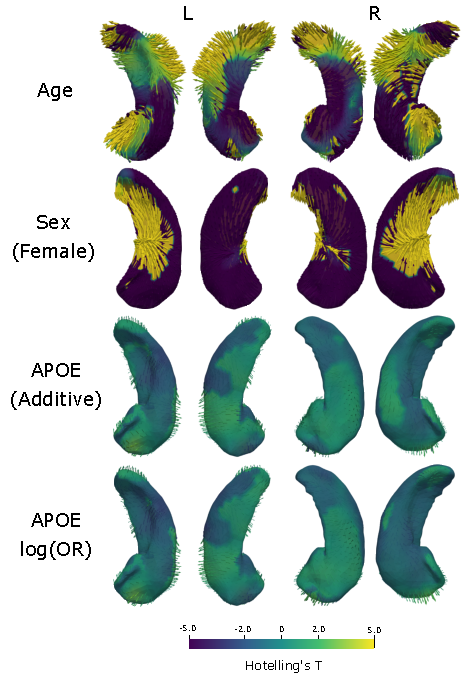
\includegraphics[width=0.9\textwidth,height=0.9\textheight,keepaspectratio]{figures/hippocampus/baseline_hippo_alfa.pdf}
  \caption[Directional effect on the surface of the hippocampus, ALFA cohort.]{Directional effect on the surface of the hippocampus for (from top to bottom) age, sex and APOE: Additive and log(OR) (odds ratio). ALFA cohort with the base model. Positive values (colored in light yellow) indicates expansion. Negative values (colored in dark violet) indicates contraction. Arrow length and size indicate a stronger effect.}\label{fig:alfabaselinefig1}
\end{figure}

For the squared interaction model, \ref{table:fullALFAtable} (lower part) shows the effects of the squared interaction between APOE OR and age, as well as the effects of the additive,  dominant and AD risk interaction terms with age and squared age, and the information about the surviving clusters in the interaction models. Figure \ref{fig:alfainteractionfig2} shows three different clusters where a significant expansion can be found on two different clusters, two on the head of the hippocampus, and a smaller one on the hippocampal tail. The first two clusters also appear on an additive interaction model (Supplementary File S5). A similar region appears when comparing HE vs NC. Figure \ref{fig:alfainteractionfig2} also shows the magnitude of the vector of the corrected effect with respect to the three peak clusters of the detected region, compared to age, for each of the alelle pairs, observing similar interactions depending on the $\varepsilon$4 allele load, with large uncertainty for the $\varepsilon$2$\varepsilon$2 subjects. \\

\begin{figure}[htbp]
  \centering
  \includegraphics[width=0.75\textwidth]{figures/hippocampus/fig_interactionapoealfa_OR.pdf}
  \caption[Quadratic interaction between APOE OR for AD and age on the right hippocampus.]{Quadratic interaction between APOE OR for AD and age on the right hippocampus after adjusting for other covariates, for all possible allele pairs. Positive values (colored in light yellow) indicates expansion. Negative values (colored in dark violet) indicates contraction. Arrow length and size indicate a stronger effect. For the interaction plots, Y(adj) is the magnitude of the adjusted $y$ variable on the detected cluster. Shaded gray areas indicate $90\%$ confidence intervals.}\label{fig:alfainteractionfig2}
\end{figure}

\subsection{ADNI dataset}

For the ADNI cohort, after preprocessing (Section \ref{sec:pipeline}) and discarding subjects with segmentation errors, we ended up with 969 patients. Supplementary Table S6 shows the ID of all ADNI subjects used in the study. \\

Table \ref{table:fullADNItable} summarizes the main results for all the experiments, using the models described in Section \ref{subsec:exp}. "Base model" section shows the effects for age, sex, site, years of education, APOE and DX. Figure \ref{fig:adnibaselinefig1} shows the effects of selected factors on the surface of both hippocampi. Similar to what happened in ALFA, age and sex present a general contraction over all the surface. DX and APOE also show a general contraction effect. No significant clusters were found on the effect of acquisition site. "Interactions" section of Table \ref{table:fullADNItable} shows results of models with and squared interactions between APOE and age, and between DX and age. For the interaction model between age and diagnosis, no significant clusters were detected. Full results for the interaction model between age and diagnosis and diagnosis and APOE are included in Supplementary Tables S7 and S8. \\

\begin{table}[htbp]
\centering
\resizebox{0.9\textwidth}{!}{%
\begin{tabular}{@{}c|c||ccc||ccc@{}}
\toprule
 & \multirow{2}{*}{Test} & \multicolumn{3}{c||}{Results}  & \multicolumn{3}{c}{Cluster analysis} \\  \cline{3-5} \cline{6-8}
 &  & Hipp & Avg. T & Max. T & N & $P_{peak}$ & $P_{cluster}$ \\ \midrule
\multirow{17}{*}{\rotatebox[origin=c]{90}{Base model}} & Age &    R &  1.76 &   13.45 & 2379 &   $<0.001$ &  $<0.001$  \\
&    &    L &   1.75 &  14.3 & 2185 &    $<0.001$ &  $<0.001$ \\
& Sex    &    R &  2.19 &  12.85 &  2488 &  $<0.001$ & $<0.001$ \\
&       &    L &   2.17 &  13.73 & 2375 &   $<0.001$ & $<0.001$ \\
& Site &    R &    0.64 &   3.60 &  - & - & - \\
&      &    L &   0.65 &   3.24 & - & - & - \\
& Years ed. &    R & 0.80 &   4.33 &  109 &   0.029 &  0.003 \\
&           &    L & 0.73 &   4.06 &  - & - & - \\
& APOE (Add) &   R &    0.9 &  5.1 &  234 & 0.001  & $<0.001$  \\
&                         &   &   &    & 144 & 0.013 &  0.003 \\
&              &    L &   1.02 &   6.38 &   529 &  $<0.001$ &  $<0.001$ \\
&              &     &    & &   304 &  $<0.001$ &  $<0.001$ \\
& APOE ($\log$(OR)) &   R &   0.92 &   5.06 & 476 &  0.002 &  $<0.001$ \\
&           &   L &   1.04 &   6.34 &  1223 &    $<0.001$  &   $<0.001$  \\
& DX (AD>MCI>CN) &   R &   1.65 &  10.10 & 2383 &     $<0.001$  &   $<0.001$  \\
&                &   L &   1.65 &  11.59 &  2289 &  $<0.001$  &  $<0.001$  \\ \midrule
\multirow{14}{*}{\rotatebox[origin=c]{90}{Interactions}} & APOE (Add)$\times$Age &    R & 0.58 &   3.02 & - & - & -  \\ 
&                     &    L &   0.68 &   3.54 & - &  - & - \\ 
& APOE (Dom)$\times$Age &    R &   0.6 &   2.87  &  - & - & - \\ 
&                     &    L &   0.72 &  3.54 & - &  - & - \\
&  APOE (Add)$\times$Age$^2$ &    R &   0.55 &   3.06 &  - & - & - \\ 
&                         &    L &    0.64 &   3.42  &  - & - & - \\ 
& APOE (Dom)$\times$Age$^2$ &    R &   0.56 &   2.91   &  - & - & - \\ 
&                        &    L &    0.65 &   3.51 & - & - & - \\ 
& APOE ($\log$(OR)))$\times$Age$^2$ &    R & 0.54 & 2.74 &  - & - & - \\ 
&                        &    L & 0.6  & 3.29  & - & - & - \\ 
& APOE ($\log$(OR)))$^2\times$DX &  R & 0.65 & 3.17 &  - & - & - \\ 
&                        &    L & 0.7  & 3.94 & - & - & - \\ 
& (AD > MCI) $\times$Age$^2$ &    R &   0.71 &  3.38   &  - & - & - \\ 
&                          &    L &    0.75 &   3.84 & - &  - & - \\  \bottomrule
 \bottomrule
\end{tabular}}
\caption[Results obtained on the ADNI cohort for base, linear interaction, and squared interaction models.]{Results obtained on the ADNI cohort for base, linear interaction, and squared interaction models. General test results and information about significant clusters that survived correction are included. Results are divided by model (base, linear interaction or squared interaction). Hipp indicates left (L) or right (R) hippocampus. Max. and Avg. T are the maximum and average Hotelling's T statistic over all vertices, respectively. XX > YY indicates the comparison used for that specific test. For the cluster analysis after correction, N is the number of vertices of the significant cluster. $P_{peak}$ and $P_{cluster}$ are the random field corrected p-values for the peak point and the whole cluster, respectively. Only  clusters with N > 20 and $P_{cluster} < 0.05$ are included. DX: diagnosis. Rec: recessive. Add: additive. Dom: dominant. OR: Odds risk.}\label{table:fullADNItable}
\end{table}

\begin{figure}[htbp]
  \centering
  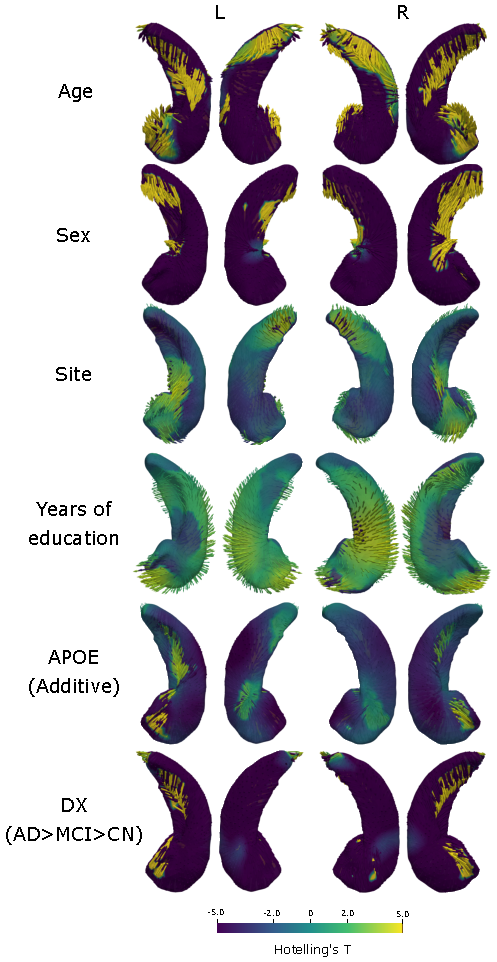
\includegraphics[width=0.75\textwidth]{figures/hippocampus/baseline_hippo_adni.pdf}
  \caption[Directional effect on the surface of the hippocampus, ADNI cohort.]{Directional effect on the surface of the hippocampus for (from top to bottom) age, sex, site, years of education, APOE and DX. ADNI cohort with the base model. Positive values (colored in light yellow) indicates expansion. Negative values (colored in dark violet) indicates contraction. Arrow length and size indicate a stronger effect.}\label{fig:adnibaselinefig1}
\end{figure}
%htbp

On comparison between healthy patients, ADNI includes 256 cognitively healthy patients, with a relatively low proportion of $\varepsilon4$-homozygotes (6 patients, less than $5\%$). For this reason, it is difficult to extract meaningful conclusions from the experiments. We tested for main effects and interactions between APOE and age to detect any similarities to the results obtained in ALFA, considering that the obtained results will not have enough statistical power to draw meaningful conclusions. Supplementary file S9 shows the effect on the surface of the hippocampus for APOE and interaction between age and APOE. \\

\subsection{Similarity between effects}
\label{sec:similarity}
\definecolor{Gray}{gray}{0.9}

We quantitatively assessed the similarity between different effects obtained in our tests. Table \ref{table:sim} shows the results for the different selected comparisons. Comparisons 1 to 4 are designed to study similarities between APOE effects and DX effects, whereas comparisons 5 to 8 are aimed to study similar APOE effects across different cohorts. The most relevant comparisons, due to their relevancy or strong effect detected are highlighted in grey and shown in more detail in Supplementary Figure S10, including the effect maps for both compared effects, the full similarity map, and the significant clusters discovered after the randomization testing (Section \ref{sec:visualization}). Figure \ref{fig:sim_2} shows a comparison between effects of the square additive interaction between age and APOE in ALFA, and the effect of the negative squared interaction between age and diagnosis in ADNI, and the corresponding discovered clusters, observing strong similarities in several regions of the hippocampus for both comparisons. For further results on the similarity tests, Supplementary Table S11 shows similarities between same effects on different cohorts and Supplementary Files S12 and S13 contains the full results for all conducted tests, for the APOE $\varepsilon$4 load models and AD OR model respectively. \\

\begin{figure}[htbp]
  \centering
  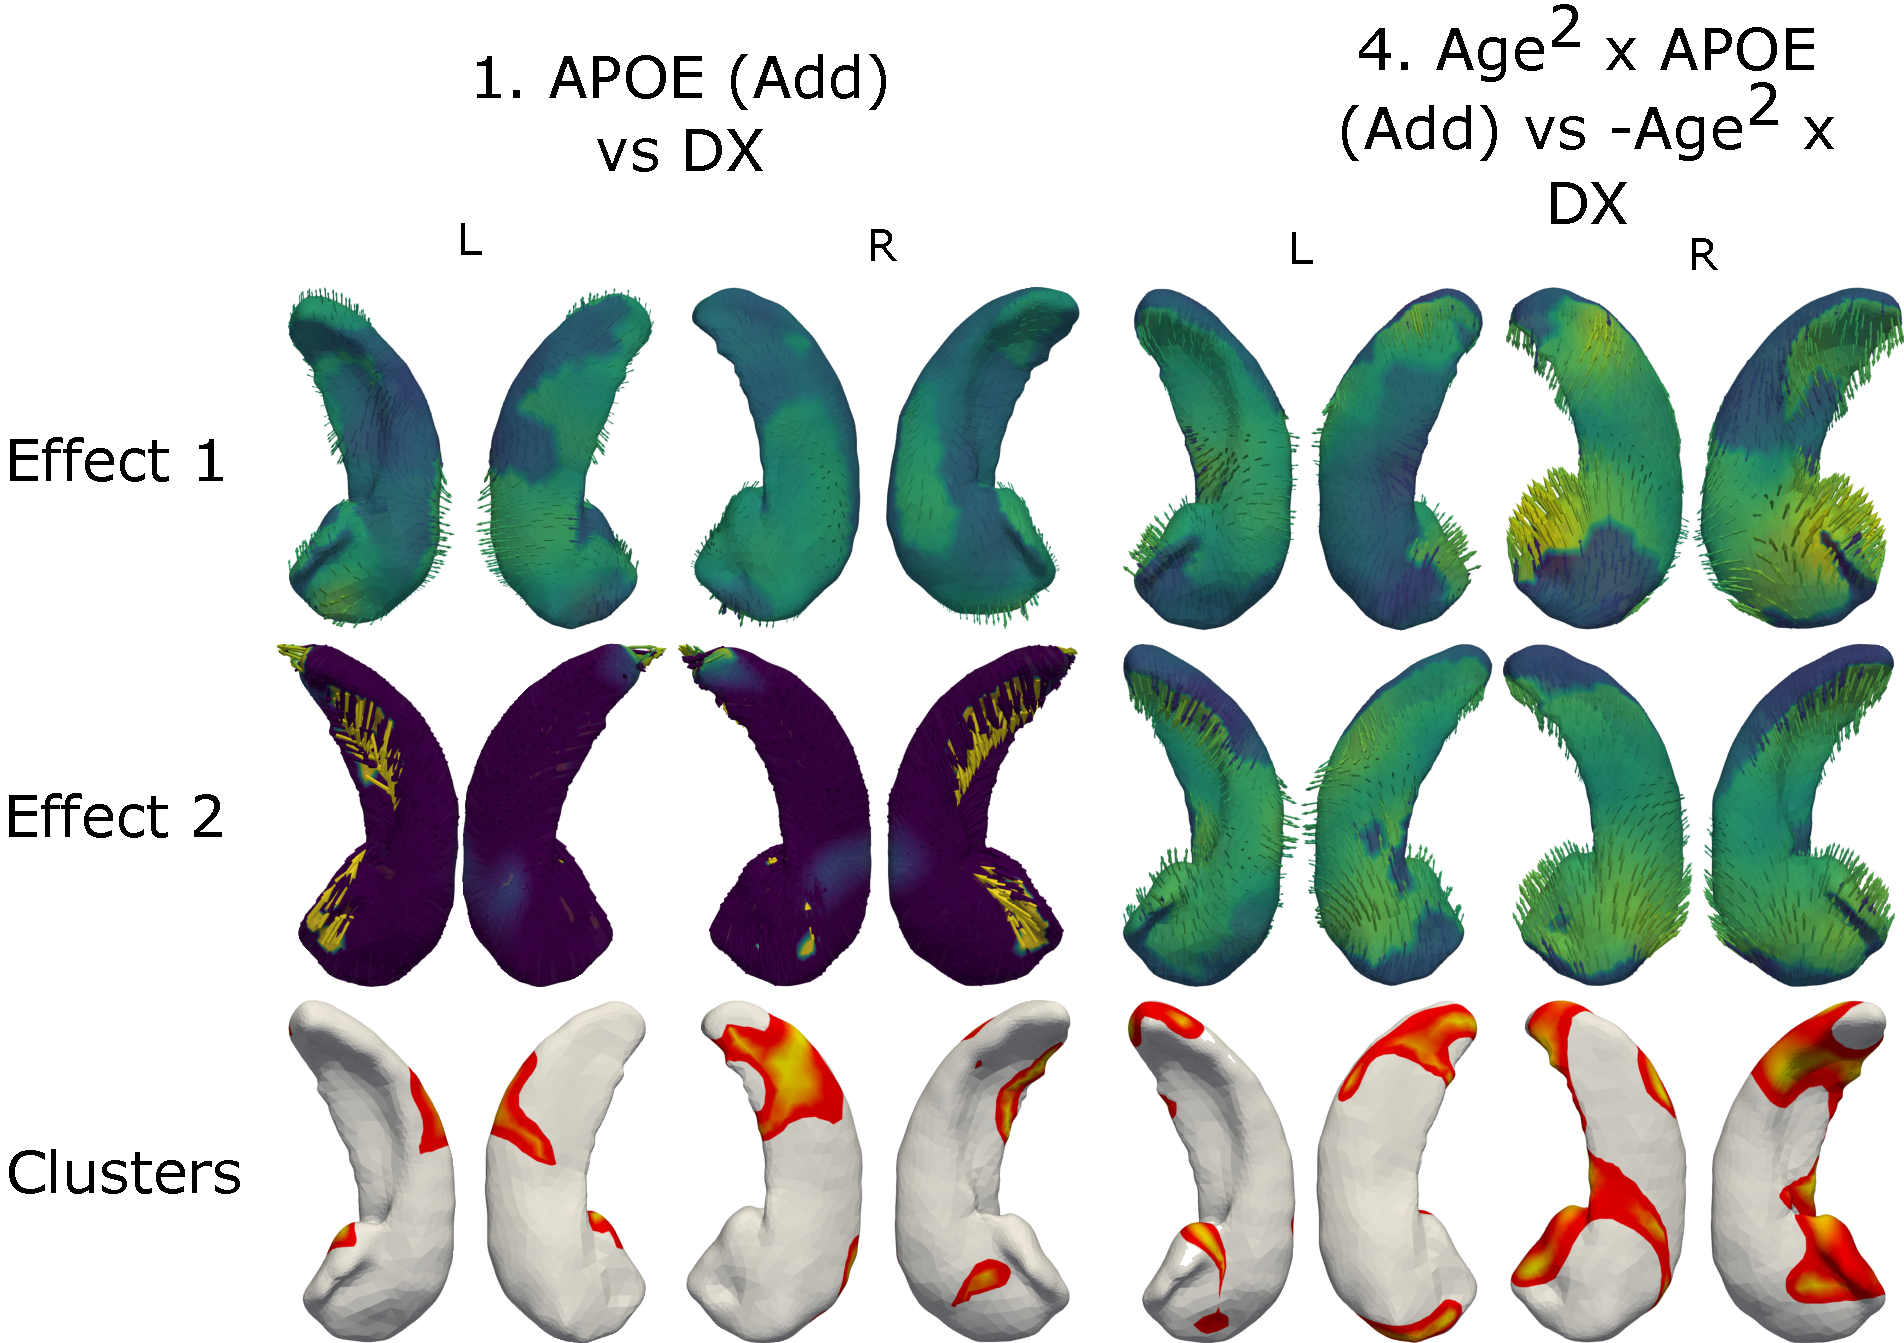
\includegraphics[width=0.8\textwidth]{figures/hippocampus/sim_figure_2.pdf}
  \caption[Effects of the squared additive interaction between age and APOE in ALFA.]{Effects of the squared additive interaction between age and APOE in ALFA dataset (above) and the effects of the negative squared interaction between diagnosis and age in ADNI (below). Both hippocampus are represented.}\label{fig:sim_2}
\end{figure}

\begin{table}[htbp]
\centering
\resizebox{0.95\textwidth}{!}{%
\begin{tabular}{@{}p{7cm}cccccc}
 \toprule
Comparison  & Effect 1 & Effect 2 & Hipp & Sim & N    & P     \\ \midrule
\multirow{10}{*}{1. ALFA base - ADNI base}  & APOE (Add)      & Age      & R    & 0.55 & 55 & 0.028\\
                              &          &          & L    & 0.51 & 72 & 0.028 \\
                              & APOE (Add)      & Years ed.      & R    & 0.61 & 109 & 0.028  \\
                              &          &          & L    & 0.56 & 234  & 0.031 \\
                              & APOE (Add)   & APOE (Add)      & R   & 0.66 & 290 & 0.026  \\ 
                              &              &                 & L   & 0.61 & 173 & 0.036 \\ 
             & \cellcolor{Gray} APOE (Add)      & \cellcolor{Gray} DX  & \cellcolor{Gray} R   & \cellcolor{Gray} 0.62 & \cellcolor{Gray} 268 & \cellcolor{Gray} 0.021 \\ 
           &   \cellcolor{Gray}         &   \cellcolor{Gray}       &  \cellcolor{Gray} L    & \cellcolor{Gray} 0.58 & \cellcolor{Gray} 213 & \cellcolor{Gray} 0.022 \\  
             &  APOE ($\log$(OR))  & APOE ($\log$(OR))  & R   & 0.56  & 79 & 0.022 \\ 
           &       &          & L    & 0.58 & 221 & 0.014 \\  \midrule
%%% 2
\multirow{6}{*}{2. ALFA (linear int.) - ADNI base}  & \cellcolor{Gray} Age$\times$APOE (Add) & \cellcolor{Gray} DX  & \cellcolor{Gray} R    & \cellcolor{Gray} 0.60 & \cellcolor{Gray} 239 & \cellcolor{Gray} 0.025 \\
      &  \cellcolor{Gray}   & \cellcolor{Gray}  & \cellcolor{Gray} L & \cellcolor{Gray} 0.49 & \cellcolor{Gray} 96  & \cellcolor{Gray} 0.020 \\
                               & Age$\times$APOE (Add) & APOE (Add)  & R  & 0.57 & 212 & 0.023 \\
                           &          &          & L    & 0.54 & 92  & 0.022 \\
%                               & AgexAPOE (Add) & Age  & R  & 0.7 & 295 & 0.02  \\
%                           &          &          & L    & 0.49 & 39  & 0.02 \\
       & \cellcolor{Gray} Age$\times$APOE (Dom) & \cellcolor{Gray} APOE (Dom)  & \cellcolor{Gray} R    & \cellcolor{Gray} 0.59 & \cellcolor{Gray} 233 & \cellcolor{Gray} 0.024 \\
     &    \cellcolor{Gray}  & \cellcolor{Gray} & \cellcolor{Gray} L    & \cellcolor{Gray} 0.51 & \cellcolor{Gray} 109  & \cellcolor{Gray} 0.021 \\ \midrule
%%% 2.2
\multirow{8}{*}{3. ALFA (sq int.) - ADNI base} & \cellcolor{Gray} Age$^2$xAPOE (Add) & \cellcolor{Gray} DX  & \cellcolor{Gray} R    & \cellcolor{Gray} 0.50 & \cellcolor{Gray} 154 & \cellcolor{Gray} 0.021 \\
  & \cellcolor{Gray}  & \cellcolor{Gray} & \cellcolor{Gray} L    & \cellcolor{Gray} 0.62 &\cellcolor{Gray} 273  & \cellcolor{Gray} 0.019 \\
                               &  Age$^2$xAPOE ($\log$(OR)) & DX  & R  & 0.60 & 131 & 0.022 \\
                                &         &          & L    & 0.63  & 275 & 0.019 \\
                               & Age$^2\times$APOE (Add) & APOE (Add)  & R    & 0.50 & 187 & 0.023 \\
                               &          &          & L    & 0.58 & 240  & 0.019 \\
                               & Age$^2\times$APOE (Dom) & APOE (Dom)  & R    & 0.50 & 199 & 0.019 \\
                               &          &          & L    & 0.53 & 213  & 0.019 \\ \midrule
%%% 3
\multirow{4}{*}{4. ALFA (sq int.) - ADNI (sq int.)} & \cellcolor{Gray} Age$^2\times$APOE (Add) & \cellcolor{Gray} -Age$^2\times$DX  & \cellcolor{Gray} R    & \cellcolor{Gray} 0.87 & \cellcolor{Gray} 686 & \cellcolor{Gray} 0.022 \\
                  &  \cellcolor{Gray}   &  \cellcolor{Gray} & \cellcolor{Gray} L    & \cellcolor{Gray} 0.81 & \cellcolor{Gray} 274  & \cellcolor{Gray} 0.028 \\ 
&  \cellcolor{Gray} Age$^2\times$APOE ($\log$(OR)) & \cellcolor{Gray} -APOE ($\log$(OR)) $\times$DX  & \cellcolor{Gray} R    & \cellcolor{Gray} 0.68 & \cellcolor{Gray} 218 & \cellcolor{Gray} 0.02 \\
                  & \cellcolor{Gray}  & \cellcolor{Gray}  & \cellcolor{Gray} L    & \cellcolor{Gray} 0.66 & \cellcolor{Gray} 270 & \cellcolor{Gray} 0.02 \\ \midrule
%% 4
\multirow{2}{*}{5. ALFA base - ADNI NC base} & \cellcolor{Gray} APOE (Add)   & \cellcolor{Gray} APOE (Add)  & \cellcolor{Gray} R   & \cellcolor{Gray} 0.70 & \cellcolor{Gray} 169 & \cellcolor{Gray} 0.026  \\ 
                              & \cellcolor{Gray}   & \cellcolor{Gray} &  \cellcolor{Gray} L   & \cellcolor{Gray} 0.61 & \cellcolor{Gray} 201 & \cellcolor{Gray} 0.023 \\ \midrule
%%% 5.1
%\multirow{4}{*}{6. ALFA (lin int.) - ADNI NC (lin. int)}  & AgexAPOE (Add) & AgexAPOE (Add)  & R  & 0.37 & 212 & 0.02 \\
%                               &          &          & L    & 0.36 & 92  & 0.02 \\
%                               & AgexAPOE (Dom) & AgexAPOE (Dom)  & R    & 0.39 & 233 & 0.02 \\
%                               &          &          & L    & 0.34 & 109  & 0.02 \\ \midrule
%%% 5.2
\multirow{2}{*}{6. ALFA (sq int.) - ADNI NC (sq int.)} & Age$^2\times$APOE (Dom) & Age$^2\times$APOE (Dom)  & R    & 0.53 & 190 & 0.033 \\
                               &     &          & L    & 0.44 & 35 & 0.021 \\ \midrule
%%% 6
\multirow{4}{*}{7. ALFA base - ALL base}  &  APOE (Add)      & DX   & R   & 0.63 & 260 & 0.021 \\ 
                              &      &          & L    & 0.58 & 206 & 0.024 \\
                              &   APOE (Dom)      & APOE (Dom)   & R   & 0.57 & 155 & 0.030 \\ 
                              &       &          & L    & 0.62 & 135 & 0.036 \\ \midrule
%%% 7
\multirow{2}{*}{8. ALFA (sq int.) - ALL (sq int.)}     & Age$^2\times$APOE (Dom) & Age$^2\times$APOE (Dom)  & R  & 0.34 & - & - \\
                               &          &          & L    & 0.36 & 20 & 0.019 \\ \bottomrule 
\end{tabular}}
\caption[Similarity results between effects.]{Similarity results between effects. Hipp indicates left (L) or right (R) hippocampus. Sim is the mean similarity for all vertices. XX > YY indicates the comparison used for that specific test. N is the number of vertices of the significant cluster. P is the mean p-value of the significant cluster. Only the largest detected cluster of each test is included in the table. Only clusters with N > 20 and $P_{cluster} < 0.05$ are included. DX: diagnosis. Add: additive. Dom: dominant. Rows highlighted are shown in more detail in Supplementary Figure S10.}\label{table:sim}
\end{table}

\section{Discussion}
\label{sec:discussion}

%%% 0 introducció.
In this article we investigated the effect of APOE $\varepsilon4$ allele load on the surface of the hippocampus. We used multiple linear regression to single out the effect of covariates over the hippocampal surface and analyzed linear and non-linear interactions between APOE $\varepsilon$4 allele load and age on the hippocampal surface, while taking into account the reduced risk associated with the $\varepsilon$2 allele. We worked with a cohort of cognitively unimpaired subjects with high genetic risk (ALFA). We additionally applied our processing pipeline to a different dataset with subjects at different stages of the disease (ADNI), to study if the interactions and the APOE effect detected in ALFA can be related to the effect of the disease in individuals along the disease continuum. We show some areas of the hippocampus where APOE $\varepsilon$4 effect is comparable to the effect of the disease, suggesting that those regions could be affected in a similar way by APOE before disease onset. To our knowledge, this is the first study that explores interactions between APOE $\varepsilon4$ and age on hippocampal surface using an homozygote enriched dataset of healthy subjects, and compares the result to a dataset of subjects at various stages of the disease. \\

%% 1 Troballes principals del efecte APOE en ALFA. Discutir efectes additius vs domuninats o recessius. 
When adding a linear interaction term to our model for the ALFA dataset between additive APOE effect and age, we detected significant effects (Table \ref{table:fullALFAtable}, linear interaction model) in the CA1 of both hemispheres (Supplementary Figure S3, S4) \footnote{We use the hippocampal subfield map from \cite{Iglesias2015} as reference.}. It is worth noting that this effect, while appearing using a dominant model, is not significant when encoding the AD odds risk model. When adding a squared interaction to the model, APOE OR interactions with age and age squared presented strong effects in the CA1, parasubiculum and GC-DG, and on a zone between CA3, CA1, and HATA of the right hippocampus (Figure \ref{fig:alfainteractionfig2}). When observing the interaction in those zones, we see that they are grouped with respect to APOE $\varepsilon$4 allele load (Figure \ref{fig:alfainteractionfig2}, bottom), although the interaction with $\varepsilon$2$\varepsilon$2 has large uncertainty due to the low number of samples (Table \ref{table:apoeallele}). Those results were also observed when using a simpler additive model, although the smallest cluster is not detected (Supplementary Figure S5). Those areas were also detected when comparing HE to NC. However, dominant and recessive models did not detect significant clusters on those areas. \\

Findings agree with previous studies on the effect of APOE on hippocampus volume \cite{Pievani2011,Mueller2009,Cacciaglia2018}, where strong interactions between APOE $\varepsilon$4 alelle load and hippocampal volume on cognitively unimpaired subjects were detected. Going beyond those results, we have been able to suggest specific areas where that interaction is stronger, suggesting that the way in which age affects hippocampal morphology depends strongly on the APOE allele, something that has also been detected by other researchers \cite{Shi2014}. Such effects can be interpreted as if the interaction between APOE and age is different between hippocampi: there is a linear interaction in both hippocampus, and in the right hippocampus, APOE and age present significant interactions that has less impact at a higher age. Regarding the protective effect of $\varepsilon$2, we could not observe a significant effect on our experiments, given the similarity of the interaction with pairs with and without $\varepsilon$2 and the uncertainty due to the low amount of $\varepsilon$2$\varepsilon$2 samples (Figure \ref{fig:alfainteractionfig2}, bottom). \\

Without introducing interactions in ALFA, APOE does not seem to capture large variations in shape, and indeed, no clusters survived correction (Table \ref{table:fullALFAtable}), in any of the tested APOE models. Subtle differences between APOE groups cannot be easily detected on surface-based studies of the hippocampus, something also observed in other studies with a different cohort of patients \cite{Dong2019}, where such differences were subtle, even before correction. Age presented large effects over the whole surface, being most of them significant after correction, as shown in Table \ref{table:fullALFAtable} and Figure \ref{fig:alfabaselinefig1}, an expected result given that age is a known factor affecting hippocampus shape and volume \cite{Lind2006}, and the association between sex and intracraneal volume. \\ 

Our tests in the ADNI dataset show that the pipeline and the analysis methods are able to capture changes and deformations that agree with current knowledge of the effect that AD has on the hippocampus (Table \ref{table:fullADNItable}). We observed that age, sex, years of education, and site present significant differences after correction in large regions of bilateral hippocampi. Differences between AD stages were also strong, showing a general contraction over all the surface of the hippocampus (Figure \ref{fig:adnibaselinefig1}), showing the atrophy caused by the disease. APOE effect also presented a general atrophy effect over all the surface, similar to the AD effect. This similarity can be explained by the unequal distribution of patients for each diagnosis (Table \ref{table:cohorts}), with demented patients having higher APOE based risk. We did not find any significant interactions between APOE $\varepsilon$4 and age in ADNI (Table \ref{table:fullADNItable}). We did find an interaction between APOE $\varepsilon$4 and DX on the left hippocampus between AD and MCI groups (Table \ref{table:fullADNItable}), but no other significant results with any other contrasts (Supplementary Table S8), which suggests that APOE $\varepsilon$4 impacts the three tested stages of AD in a similar way, with a small interaction between MCI and AD. We also tested for interaction between APOE OR and AD diagnosis to see if a protective effect of $\varepsilon$2 could appear, but no significant interaction were found. \\

Apart from the already mentioned findings on age and APOE interaction on ALFA dataset, we have not detected large differences between our different model encodings of the allele information. Recessive and dominant models did not reveal further zones or interactions that were not already detected by the other models, and additive models (Supplementary Figure S5) and AD OR models (Figure \ref{fig:alfainteractionfig2}) were the most informative models. Effects maps and results were also very similar between models (Table \ref{table:fullALFAtable}, Figure \ref{fig:alfabaselinefig1}). This indicates that the effect of APOE $\varepsilon$4 allele load could be modelled more appropriately in a linear (additive) way, or encoding empirical knowledge of the risk to the model \cite{Reiman2020}. \\

We studied the similarities between APOE $\varepsilon$4 effects and DX effects over ALFA and ADNI cohorts. Results between the same effects (e.g. age vs age, sex vs sex) on different cohorts (shown in Supplementary Table S10) show high similarities, showing that results are comparable between cohorts. Table \ref{table:sim} (comparisons 1-4) show that, for baseline effects, there are some areas on the tail and presubiculum of the hippocampus where a high similarity can be found, with significant clusters detected in the right hippocampus. This could indicate that, even if in our previous tests those regions did not have a strong enough statistical power, APOE $\varepsilon$4 could affect those regions before the onset of the disease, and leave them more vulnerable to the atrophy caused by AD, which is consistent with existing literature on this relationship \cite{Wolk2010}. However, as previously mentioned, AD and APOE $\varepsilon$4 effects on ADNI (observed in Figure \ref{fig:adnibaselinefig1}) have a general atrophy effect over all the surface, so the found significant areas could simply be regions where APOE produces a contraction effect. We found a large similarity in the interaction effect between squared age and APOE in the ALFA dataset and the inverse interaction effect between squared age and diagnosis in ADNI, with several large significant clusters. This result suggests that age modulates the effect of both APOE and DX over a specific local area on the hippocampal surface in a similar way, being a direct effect for APOE and an inverse effect for DX. Figure \ref{fig:sim_2} shows a larger version of both effect maps, where the similarities between effects can be better appreciated. Similarity is specially high on the right hippocampus, where the interaction between APOE and age in CN subjects is significant (Figure \ref{fig:alfainteractionfig2}). Comparing the similarities obtained using the APOE odds risk model, they are very similar to the ones obtained using additive/dominant models, in line with previous observations (Supplementary Tables 12 and 13).  \\ 

We tested our methods on a subset of the ADNI dataset, to be able to directly compare two different cohorts of cognitively healthy patients, and we also did additional analysis by combining both cohorts. Table \ref{table:sim} (comparisons 5 to 8) shows the obtained results. We compared between APOE effects, between APOE and DX effects, and between interactions. Similar areas were found, but the detected significant clusters are small and non-conclusive. For the combination of cohorts, no significant results were found (Supplementary Tables S1 and S2, and Supplementary Figures S14 and S15). This lack of significant results could suggest that the interaction effect detected in ALFA is strongly influenced by the $\varepsilon4$ homozygotes, of which the ADNI cohort has a lower proportion. \\ 

We conjecture three (non-exclusive) reasons for the results obtained in those comparisons. First, the site variable for the combined cohort (we added a new category for ALFA subjects) captured much more variation than in previous tests with only ADNI patients, where differences were not significant. This variation shows that differences in image acquisition and protocols between sites greatly influence the obtained MRI and hence the obtained hippocampus mesh. Second, the age disparity between datasets (Supplementary Figure S16). ADNI individuals are older than ALFA ones, due to differences in study recruitment and aim (ALFA focuses on cognitively healthy subjects, with no signs of the disease, whereas ADNI focuses on subjects that are already in the AD continuum). This difference in the age distribution could also explain why detected interactions in ALFA are not present in ADNI, should such interactions only happen (or be more apparent) at an earlier age. Finally, there could exist other population differences that are not being accounted for. \\

%% Limitacions.
Our study presents various limitations. First, even if our analysis allows for testing any effect on the surface of the hippocampus, we focused on APOE $\varepsilon$4 allele load and interactions with age. We could add to our analysis other risk factors, such as relevant genotypic factors, cognitive scores, or lifestyle and cardiovascular factors. One key advantage of ADNI over ALFA at this stage is the availability of biomarker status on cerebrospinal fluid. $A\beta$ levels in ADNI could be used to disentangle whether differences observed in ALFA might be due to abnormal amyloid levels or interactions with such levels. However, previous reports have determined that the impact of amyloid accumulation on morphological changes in the brain of cognitively unimpaired individuals is low, a well as any interactive effects of APOE $\varepsilon$4 \cite{Liu2015c,Lim2017}. For multimodal analysis, methods such as multiple kernel learning, which has been used on other types of medical data for disease characterization, could be used \cite{Sanchez-Martinez2017,Marti-Juan2019}. Another interesting line of work is to directly study the deformations and effects that happen at the different hippocampus subfields, similar to \cite{Zhao2019}. Second, our analysis were limited to the hippocampus region, but we could extend them to other parts of the brain that present differences in healthy subjects, such as the ventricles. Third, given the large effect of the site in our analysis, segmentation should be improved to ensure robust comparisons between datasets. Moreover, we only used cross-sectional data. Extending our analysis to a longitudinal cohort may allow us to test the shape changes over time, which could also be affected by APOE $\varepsilon$4. \\

\section{Conclusions}
\label{sec:conclusions}

In this article, we have studied differences in hippocampal surface shape on a cohort of genetically enriched cognitively healthy subjects. We have shown a linear and quadratic interaction between APOE $\varepsilon$4 allele load and age on two different surface regions of the right hippocampus. We have also applied the same method on a different cohort of subjects (including both cognitively impaired and unimpaired subjects), and detecting remarkable similarities between the APOE interaction with age in asymptomatics and the effect of the disease in a second cohort. Results suggest that for late/middle-aged cognitively unimpaired subjects, APOE $\varepsilon$4 exerts an effect on the hippocampal surface comparable to that observed in clinical stages of AD but to a lower extent. In addition, these effects interacted with age, showing a remarkable similarity across the two studied cohorts. \\

\section*{Acknowledgements}
This publication is part of the ALFA study (ALzheimer and FAmilies). The authors would like to express their most sincere gratitude to the ALFA project participants, without whom this research would have not been possible. The project leading to these results has received funding from “la Caixa” Foundation (ID 100010434), under agreement LCF/PR/ GN17/50300004. Additional support has been received from the Universities and Research Secretariat, Ministry of Business and Knowledge of the Catalan Government under the grant no. 2017-SGR-892. This work was also partially funded by the Spanish Ministry of Economy and Competitiveness under the María de Maeztu Units of Excellence Programme 525 [MDM-2015-0502]. JDG is supported by the Spanish Ministry of Science, Innovation and Universities - State Research Agency (RYC-2013-13054). 

Data collection and sharing for this project was funded by the Alzheimer's Disease Neuroimaging Initiative (ADNI) (National Institutes of Health Grant U01 AG024904) and DOD ADNI (Department of Defense award number W81XWH-12-2-0012). ADNI is funded by the National Institute on Aging, the National Institute of Biomedical Imaging and Bioengineering, and through generous contributions from the following: AbbVie, Alzheimer’s Association; Alzheimer’s Drug Discovery Foundation; Araclon Biotech; BioClinica, Inc.; Biogen; Bristol-Myers Squibb Company; CereSpir, Inc.; Cogstate; Eisai Inc.; Elan Pharmaceuticals, Inc.; Eli Lilly and Company; EuroImmun; F. Hoffmann-La Roche Ltd and its affiliated company Genentech, Inc.; Fujirebio; GE Healthcare; IXICO Ltd.; Janssen Alzheimer Immunotherapy Research {\&} Development, LLC.; Johnson {\&} Johnson Pharmaceutical Research {\&} Development LLC.; Lumosity; Lundbeck; Merck {\&} Co., Inc.; Meso Scale Diagnostics, LLC.; NeuroRx Research; Neurotrack Technologies; Novartis Pharmaceuticals Corporation; Pfizer Inc.; Piramal Imaging; Servier; Takeda Pharmaceutical Company; and Transition Therapeutics. The Canadian Institutes of Health Research is providing funds to support ADNI clinical sites in Canada. Private sector contributions are facilitated by the Foundation for the National Institutes of Health (\url{www.fnih.org}). The grantee organization is the Northern California Institute for Research and Education, and the study is coordinated by the Alzheimer’s Therapeutic Research Institute at the University of Southern California. ADNI data are disseminated by the Laboratory for Neuro Imaging at the University of Southern California. Data used in precreation of this article were obtained from the Alzheimer’s Disease Neuroimaging Initiative (ADNI) database (\url{adni.loni.usc.edu}). As such, the investigators within the ADNI contributed to the design and implementation of ADNI and/or provided data but did not participate in analysis or writing of this report. A complete listing of ADNI investigators can be found at (\url{http://adni.loni.usc.edu/wp-content/uploads/how_to_apply/ADNI_Acknowledgement_List.pdf}).

\subsection*{Acknowledgments: List of ALFA Study collaborators:}
Collaborators of the ALFA study are: Eider M. Arenaza-Urquijo, Alba Cañas, Carme Deulofeu, Ruth Dominguez, Karine Fauria, Marta Félez-Sánchez, José M. González de Echevarri, Xavi Gotsens, Oriol Grau-Rivera, Laura Hernandez, Gema Huesa, Jordi Huguet, Paula Marne, Tania Menchón, Marta Milà-Alomà, Carolina Minguillon, Maria Pascual, Albina Polo, Gonzalo Sánchez-Benavides, Sandra Pradas, Aleix Sala-Vila, Anna Soteras, Marc Suárez-Calvet, Laia Tenas, Marc Vilanova, Natalia Vilor-Tejedor.

\section*{Data Availability}

Parts of the data that support the findings of this study are available from Alzheimer’s Disease Neuroimaging Initiative (ADNI). Restrictions apply to the availability of these data, which were used under license for this study. Data are available at http://adni.loni.usc.edu/ upon application. ALFA study data that support the findings of this study are available from the corresponding author upon reasonable request. 



\chapter{Conclusions} \label{ch:6-conclusions}
% I aqui puc intentar combinar les dos coses? Fer dos subchapters?
In the previous chapters of this thesis we have presented various approaches to study AD using heterogeneous data, both cross-sectional and longitudinal. In this final chapter, we present a general summary of the contributions described in the thesis, possible clinical applications, and relevant future works that arise from the contributions of the thesis.

\section{Main contributions}

We can summarize this thesis in four main contributions:

\begin{itemize}
\item Chapter \ref{ch:2-review} surveys research on ML methods for longitudinal data in AD. This review portrays a clear picture of the current research in this field: main problems, existing methods, and gaps in knowledge. We highlight three main findings: 1) a larger performance detected in methods when using multimodal data, compared to methods that used only one modality; 2) lack of interpretability and reproducibility, mainly due to black box learning models and and nonpublic datasets; and 3) a lack of unsupervised methods, with supervised methods being restricted to labelled or curated datasets. Our other contributions of the thesis try to address those points.

\item Chapter \ref{ch:3-cimlr} presents an unsupervised method that is able to cluster a cohort of AD patients using blood-based biomarkers, with each cluster having an associated blood profile. We then used cross-sectional and longitudinal MRI cortical and subcortical data to study the differences and interactions between those clusters and the disease, which showed two different presentations of the disease characterized by different blood profiles. The method used is an unsupervised approach and we use multimodal data for the analysis. It also is straightforward to interpret, as the nature of the model assigns a weight to each of the features. Characterization of different subtypes of the disease could lead to better personalized decisions.

\item Chapter \ref{ch:4-rnnvae} shows our proposed multi-channel recurrent variational autoencoder for AD progression, which is completely unsupervised. The method models a lower-dimensional subspace from multimodal and longitudinal data, generates missing modalities, and predicts future time points. The approach presented is highly flexible, is able to deal with different modalities and time points, and is also able to capture uncertainty. Those characteristics address the three points highlighted from Chapter \ref{ch:2-review}, which are important to tackle the challenges associated with longitudinal data analysis.

\item Chapter \ref{ch:5-pmhippocampus} analyses the an analysis of the relationship between APOE $\varepsilon4$ and age on the hippocampal surface of healthy, non-demented subjects. To tackle the lack of early-stage data from future AD patients, we take advantage of the unique ALFA dataset containing healthy mid-age people with increased risk of AD. We segment the hippocampus of all subjects of the cohort to generate 3D surface maps and perform a multivariate statistical analysis on age-APOE interactions, comparing our results in the healthy cohort to the results of a second separate cohort containing patients at all stages of the disease. We find similarities between the effects of APOE $\varepsilon4$ in healthy subjects and the effects of the disease on demented subjects, suggesting that APOE $\varepsilon4$ has a similar, milder effect on the hippocampal surface to AD effect. We answer a relevant question on the early development of AD, linking hippocampal surface, demographic information, and genetics, which could be relevant to develop future studies.
\end{itemize}

\section{Clinical applications}
The contributions described in the previous chapters have all relevant clinical applications and implications. Although the work described in this thesis does not have an immediate impact on clinical settings, it has several implications for clinical application that are described below. \\

% CIMLR
Our approach to the exploration of AD heterogeneity using blood-based biomarkers presented in Chapter \ref{ch:3-cimlr} has shown potential to uncover hidden subgroups or presentations of the disease using a group of blood-based biomarkers. This has some interesting implications. First, it suggests the potential of distinguishing between different presentations or progression paths of the disease with only non-invasive biomarkers, which could have important implications in personalized treatment and therapy for patients at all stages of the disease. Second, it can help uncover blood-based biomarkers that capture underlying processes related to the disease that could be candidates for other clinical studies. \\

%% RNNVAE
The reconstruction properties of the multichannel recurrent variational autoencoder proposed in Chapter \ref{ch:4-rnnvae} have also interesting clinical applications: it can provide a personalized way to reconstruct missing acquisitions during patient visits, for example. Moreover, we have also shown that the model has potential for clinical trajectory prediction. In a clinical setting, the ability to predict, with an associated uncertainty, the short-term evolution of the patient, could be of use for clinical studies and personalized medicine. \\

Finally, our study on hippocampal surface interaction with APOE and age described in Chapter \ref{ch:5-pmhippocampus} focuses on cognitively healthy patients, to discover early signs of the disease. Early characterization is important because it can facilitate early intervention. The study contributes to our understanding of how APOE $\varepsilon4$ affects the hippocampus of healthy, at risk population, and it could lead to discoveries on the specific effect of APOE$\varepsilon4$ in the brain and why and how it puts the patient at a higher risk of AD.

\section{Future work and research directions}

The contributions presented in this thesis put forward new research questions and open the door to novel research directions that could lead to new advancements and insights on ML studies on AD. We show, for each chapter, the lines of future work that we believe could be relevant for future studies. \\

The findings discussed in our longitudinal methods review in Chapter \ref{ch:2-review} which were not highlighted in the previous section have not been completely addressed in this thesis and are still open questions: the use of prior knowledge, and dataset and privacy issues. We expect future ML approaches on AD to be designed taking into account existing biological knowledge of the disease using the deluge of information available, such as biomarker dynamics or risk factors. Methods using this existing information and that could model longitudinal, multimodal data will be extremely valuable to improve the modelling of disease progression. Moreover, given the expansion of AD data initiatives and new cohorts around the world, we believe that future methods will use increasing amounts of data from separate cohorts to improve the reproducibility and generalization of the methods. To solve privacy concerns and other related issues that arise while working on multisite data, techniques like federated learning \cite{Yang2019} are promising.\\

The disease presentations shown in Chapter \ref{ch:3-cimlr} require validation in other cohorts to confirm and expand the possible subtypes of the disease linked to blood-based biomarkers. Further exploration could be made by using longitudinally acquired blood biomarkers, together with whole-brain voxel-based analysis, to find more specific differences between the presentations of the disease. Exploration of blood-based biomarkers for AD, either for subtyping or for diagnosis, is a line of research with recent strong results \cite{Cullen2020,Moscoso2020}, and, given their characteristics (rapid and non-invasive acquisition), it could lead to important discoveries in the coming years. \\

The generative model described in Chapter \ref{ch:4-rnnvae}, while very flexible and promising, was only recently developed and there is still potential for improvements in many aspects. We could explore multiple changes in the architecture and additional assumptions, such as incorporating time between acquisitions, extending hyperparameter and architecture exploration to improve the predictive performance, and adding more data modalities. Moreover, we have not fully explored the uncertainty the model provides, which is important for prediction models in medical settings. \\

Finally, the analysis on the hippocampus presented in Chapter \ref{ch:5-pmhippocampus} could be extended to further validate and interpret the findings. We propose two direct lines of work: analyze the hippocampal shape change over time for the same cohort, to see if temporal deformations also present differences; and conduct the analysis on the hippocampal subfields to discover the specific regions of the hippocampus where the discovered effect is present. Further research on datasets of cognitively healthy subjects such as the one used in the study is necessary to deepen the understanding of the disease at its early stages and reveal its dynamics. The effect of APOE $\varepsilon4$ on other parts of the brain that could be affected by similar effects could also be an important line of research. New methods would need to be specifically designed to capture the subtle changes caused by the disease before any cognitive decline, and they could be extremely useful to characterize the dynamics of early AD.

%% AFTER BIBLIOGRAPHY, NEED TO PRINT CV AND PUBLICATIONS?
\backmatter

%\chapter{Appendix}
% I aqui puc intentar combinar les dos coses? Fer dos subchapters?
% 
\section{Alzheimer's Disease assessment and markers}
\label{biomarkers}

% Severity of Alzheimer's Disease.
Alzheimer's Disease (AD) is characterized by a progressive degeneration of the brain and cognitive functions \cite{Lane2018}. In the literature, diagnosis of patients is usually divided in three stages \cite{Brookmeyer2007}, although other classifications have been recently proposed (Section \ref{nia}):

\begin{enumerate}\itemsep5pt
\item Healthy Control or Cognitively Normal (CN), when the patient shows neither signs of the disease nor cognitive problems.
\item Mild Cognitive Impairment (MCI), when the patient shows signs of cognitive impairment. It can be divided into two substages: early MCI and late MCI, differentiating between patients by their degree of cognitive impairment.
\item AD, when the patient is considered to have completely progressed into full-blown dementia.
\end{enumerate}

Figure \ref{appendix:figAD} shows an MRI axial view of two different patients: one healthy control and the other with AD. We can appreciate the effects of the disease directly on the reduction of cortical thickness, among other visual and physical cues \cite{Schmidt1992}. \\

\begin{figure}[htbp]
  \centering
  \includegraphics[width=0.75\textwidth]{figures/review/FigA.1.pdf}
  \caption{Axial view of MRI scan for AD (left) and CN (right) patients. Images from ADNI dataset, registered to a common template.}
  \label{appendix:figAD}
\end{figure}

\subsection*{AD markers} 

To determine the stage of the disease, various markers describing key pathophysiological processess of AD have been proposed over the years. Markers of the brain provide information for the study of the disease and its screening. AD is characterized by protein amyloid-beta (A$\beta$) deposition in the brain \cite{Rissman2012}, tau injury, and structural neurodegeneration \cite{Jack2013}. Those three indicators precede cognitive impairment, leading to death. For the measurement of these indicators, different markers have been proposed:

\begin{enumerate}\itemsep5pt
\item Brain A$\beta$ deposition in the brain can be detected both in positron emission tomography (PET) imaging \cite{Clark2011}, and in cerebrospinal fluid (CSF) \cite{Andreasen1999}.
\item Tau injury and dysfunction caused by tau and p-tau plaques, found in tau-PET imaging and CSF \cite{Andreasen1999,Blennow2010}.
\item Neurodegeneration provoked by tau injury. It can be observed in structural magnetic resonance imaging (MRI) \cite{Weiner2005} and in fludeoxyglucose (FDG)-PET imaging \cite{Chetelat2003}.
\item Memory and cognition, measured by cognitive tests.
\end{enumerate}

%% Screening
The main screening tool for clinical assessment of AD is the clinical interview between the patient and the doctor, where the severity of the cognitive problems of the patient can be assessed, followed by a cognitive physical examination to capture the aforementioned markers and assess the presence of the disease \cite{Lane2018}. \\

Apart from the aforementioned markers and imaging techniques, resting-state electroencephalography (EEG) signals have also been proposed for AD assessment \cite{Al-Qazzaz2014,Bhat2015}. However, they are not as widely used as image-based examination, as EEG cannot be used to observe specific processes in the brain and they only show changes in brain activity, which could be caused by other pathologies. A review on EEG methods for AD can be found in \cite{Houmani2018}.

\subsection*{Longitudinal marker dynamics and disease model}

The previous markers can be studied and modelled longitudinally. Modelling their trajectories and progression can give us more insight on how they change and interact. For example, longitudinal data analysis on MRI allows us to calculate the rate of change of specific brain structures, such as the dynamics of cortical and hippocampal atrophy. \\

A widely accepted progression model of AD was proposed by \cite{Jack2010}. Their model is based on marker evolution, where each marker progresses from normal values to abnormal values differently. The order of the markers is the presented above: A$\beta$ deposition, followed by tau injury, neurodegeneration and cognition. Empirical data and experiments reviewed in \cite{Jack2013} confirm the validity of the model, although other data-driven works do not fully agree with it \cite{Iturria-Medina2016}. Analyzing those markers longitudinally allows us to study both the individual and whole population rate of change, and improve AD progression modelling. \\

% PET imaging can show A$\beta$ deposition in the brain, metabolic activity, and tau concentration. PET imaging uses tracers to bind to a molecule of interest, and different measures are obtained with different tracers. Markers extracted from PET images can detect progression of the disease prior to structural changes. \\
% In cross-sectional studies, it has been shown that combining data coming from different sources improves classification results \cite{Rathore2017}. In longitudinal studies, each of the modalities can have acquisitions over time that should account for its temporal change.

\subsection*{Studies and initiatives} 
\label{biomarkers:studies}
%% Explain about studies that focus on longitudinal data. and about the challenges that promote the use of longitudinal data for progression of the disease.

There has been a remarkable number of initiatives to promote using longitudinal data on AD modelling. Availability of patients' longitudinal data is key to study the progression of the disease. \cite{Lawrence2017} presented a review of available longitudinal AD biomarker datasets, finding that more efforts are needed to increase the follow-up duration, increase the population sizes and standardize the acquisition methods. One of the largest studies is the Alzheimer's Disease Neuroimaging Initiative (ADNI) \cite{Mueller2005}, a multimodal, ongoing longitudinal study with hundreds of enrolled subjects, gathering imaging data, cognitive scores, blood and CSF markers. To unify and share the available data, the Alzheimer's Association has created The Global Alzheimer’s Association Interactive Network (GAAIN) \footnote{\url{http://www.gaain.org}} to share data between independent studies and build collaborations to create and explore large, heterogeneous cohorts. \\

% ADD MIRIAD Challenge
Initiatives to stimulate research on the field have also been proposed, such as the MIRIAD challenge \cite{miriad}, The Alzheimer's Disease Prediction Of Longitudinal Evolution (TADPOLE) Challenge\footnote{\url{https://tadpole.grand-challenge.org}} or Quantitative Templates for the Progression of Alzheimer’s disease (QT-PAD)\footnote{\url{http://www.pi4cs.org/qt-pad-challenge}}. These challenges define a fixed subset of available data, making it easier to compare results, share methods and ensure reproducibility. \\

\section{NIA-AA research framework: new biological definition on AD}
\label{nia}

A new unified research framework for a biological definition of the disease was recently published by the National Institute on Aging and the Alzheimer's Association \cite{Jack2018}. This approach defines AD as a biological construct based on markers, rather than clinical symptoms of the disease such as cognitive impairments. The framework is flexible enough for the introduction of additional markers, if needed. \\

The framework groups markers in three categories: A$\beta$ deposition, pathologic tau, and neurodegeneration. This is represented as the AT(N) system, where each category can be binarized using a cut point into normal/abnormal (-/+). For each category:

\begin{itemize}
    \item \textbf{A:} A$\beta$ markers determine if a patient is in the Alzheimer's continuum, showing pathological changes but still not presenting the disease.
    \item \textbf{T:} tau deposition markers indicate whether a patient who is in the Alzheimer's continuum has the disease.
    \item \textbf{(N):} Neurodegeneration markers show structural changes in the brain that can be product of AD, but are not specific to the disease (and thus is placed in parenthese).
\end{itemize}

% Review of existing works and if there is anything longitudinal
The flexibility of the framework allows working with missing biomarker values, which is a valuable trait for a longitudinal study. We found no work (within the scope of this review) using this new biological definition on AD. The reasons could be the recentness of the framework's publication, and the need for multimodal data in a longitudinal setting, which is not as available as single modality MRI. However, we expect future studies to use this framework, as it offers clear advantages for longitudinal analysis: for example, being able to directly compare different stages of progression between patients, or extend the framework with markers that capture longitudinal progression.

\section{Challenges in longitudinal data}
\label{longanalysis}

Longitudinal data are composed of sequential data acquisitions for subjects over a period of time. This contrasts with cross-sectional studies, which focus on single acquisitions per subject. Here, we describe the main characteristics and analysis challenges that arise while dealing with longitudinal data. In Section \ref{sec:missing} we outline strategies to overcome some of them.  \\

Two sources of variability can be defined for a longitudinal study in a cohort of subjects: the inter-subject variability, i.e., the differences between observations of different subjects, and the intra-subject variability, i.e., the differences between observations of a same subject, which tend to be highly correlated compared to the former. Those two sources of variation give valuable information about the progression of the disease between- and within- subjects. In cross-sectional studies, those two variabilities are non-separable: given two samples of different subjects, it is not possible to know to what extent their variation is due to inter-subject variability or to the different stages of the disease. Adding longitudinal samples for each subject allows us to distinguish between those two variabilities, improving our understanding of the disease \cite{Fitzmaurice2008}. \\

\begin{figure}[htbp]
  \centering
  \includegraphics[width=1.0\textwidth]{figures/review/FigC.2.pdf}
  \caption{Longitudinal representation of data acquisitions for two patients.}
  \label{long}
\end{figure}

Figure \ref{long} shows an example of a longitudinal study for two subjects, with multiple data modalities, over a fixed span of time. It illustrates some of the challenges that can appear in a longitudinal, multimodal data study: \\

% The figure should include these various points
\begin{enumerate}\itemsep5pt
\item Each subject can have a different number of acquisitions, leading to an unbalanced data problem. In the figure, Patient B missed the 12th month acquisition for some reasons.
\item There can be missing data due to missing acquisitions from some modalities. In the figure, only patient A at the 6-months follow-up has all the acquisitions. 
\item Data are not necessarily acquired at the same time point for the different subjects.
\item Time spacing between follow-ups can be variable, even within a single subject.
\end{enumerate}

Another problem, not shown in the figure, is that different patients can be at different stages of the disease at a given time point. Reference time to measure progression remains an open issue in the field \cite{Ashford2001}.  \\

Protocols of data acquisition try to palliate these problems, but in a clinical setting, this is very difficult to achieve: sometimes patients miss their scheduled screening session and data cannot be gathered. Other patients might drop out from the study for a variety of reasons, such as disease severity or moving out of the city/country, and in other cases, data of a given time point could need to be discarded because of quality problems. For these reasons, most of the available longitudinal data is unbalanced. \\

All studies should define their policy on this issue, either by selecting only subjects with no missing data in their studies, or by defining a method to handle the problem. Popular methods for missing data in longitudinal studies are detailed in \cite{Ibrahim}. \\



\addcontentsline{toc}{chapter}{BIBLIOGRAPHY}
\bibliography{phdbib}

%\addcontentsline{toc}{chapter}{CURRICULUM VITAE}
%\chapter*{CURRICULUM VITAE}

\addcontentsline{toc}{chapter}{PUBLICATIONS}
\chapter*{PUBLICATIONS}

\subsection*{2021}

\begin{itemize}
\item \textbf{Martí-Juan, G.}, .... (la de MCVAE). In preparation.
\end{itemize}

\subsection*{2020}

\begin{itemize}
\item \textbf{Martí‐Juan, G.}, Sanroma‐Guell, G., Cacciaglia, R., Falcon, C., Operto, G., Molinuevo, J. L., … Piella, G. (2020). Nonlinear interaction between APOE$\varepsilon$ 4 allele load and age in the hippocampal surface of cognitively intact individuals. Human Brain Mapping, hbm.25202. \url{https://doi.org/10.1002/hbm.25202}

\item \textbf{Martí-Juan, G.}, Sanroma-Guell, G., Piella, G. (2020, June 1). A survey on machine and statistical learning for longitudinal analysis of neuroimaging data in Alzheimer’s disease. Computer Methods and Programs in Biomedicine, Vol. 189, p. 105348. \url{https://doi.org/10.1016/j.cmpb.2020.105348}
\end{itemize}

\textbf{2019}

\begin{itemize}

\item \textbf{Martí-Juan, G.}. Sanroma, G., Piella, G., 2019. Heterogeneity of longitudinal brain imaging phenotypes in Alzheimer's Disease based on based on unsupervised clustering of blood marker profiles. Computer Assisted Radiology and Surgery (CARS) Poster Presentation, Rennes 2019.

\item \textbf{Martí-Juan, G.}, Sanroma, G., Piella, G., 2019. Revealing heterogeneity of brain imaging phenotypes in Alzheimer’s disease based on unsupervised clustering of blood marker profiles. PLoS One 14. \url{https://doi.org/10.1371/journal.pone.0211121}
\end{itemize}

\printindex

\end{document}